\documentclass[tombow,dvipdfmx]{corona-a5}
% dvipdfmxを追加(川口)

% Springer document settings
\usepackage[bottom]{footmisc}% places footnotes at page bottom

\usepackage{newtxtext}       % 
\usepackage[varvw]{newtxmath}       % selects Times Roman as basic font
%%%%%%%%%%%%%%%%%%%%%%%%%%%%%%%

% \usepackage{amssymb}
\usepackage{ntheorem}
\usepackage{amsmath}
\usepackage{enumitem}


\usepackage{graphicx}
\usepackage{color}
\usepackage{cite}
\usepackage{makeidx}


\usepackage{ascmac}
\usepackage{eclbkbox}
\usepackage{dsfont}

\usepackage{longtable}

\usepackage{url}

\usepackage{hyperref}

\usepackage{multicol}

%% --川口追加--
\makeatletter
\let\MYcaption\@makecaption
\makeatother
\usepackage{subcaption}
\captionsetup{compatibility=false}      % 必要に応じて

\makeatletter
\let\@makecaption\MYcaption
\makeatother
% ----

%%
\theoremstyle{plain}
\theoremheaderfont{\bfseries}
\theorembodyfont{\rmfamily}
\theoremseparator{\hspace{1ex}}
\theoremindent0cm
\theoremnumbering{arabic}
\theoremprework{\vspace{1ex}\begin{shadebox}\vspace{1ex}}
\theorempostwork{\vspace{-1ex}\end{shadebox}\vspace{1ex}}

%%
\theoremclass{theorem}

%%
\theoremclass{theorem}

%%
\theoremclass{theorem}


%%
\theoremstyle{break}
\theoremheaderfont{\bfseries}
\theorembodyfont{\rmfamily}
\theoremseparator{}
\theoremindent0cm
\theoremnumbering{arabic}
\theoremprework{\vspace{1.5ex}\begin{breakbox}\vspace{-0.5ex}}
\theorempostwork{\vspace{-0.5ex}\end{breakbox}\vspace{1.5ex}}

%%
\theoremstyle{nonumberplain}
\theoremseparator{\hspace{1ex}}

%%
\newtheorem{assumption}{Assumption}[section]

%%
\renewcommand{\theproblem}{}

\renewcommand{\theremark}{}


\newcommand{\red}[1]{{\color{red}#1}}
\newcommand{\blue}[1]{{\color{blue}#1}}
\newcommand{\green}[1]{{\color{green}#1}}

\DeclareMathOperator*{\argmax}{arg\,max}

\newcommand{\bm}[1]{\boldsymbol{#1}}
\newcommand{\sfT}{\mathsf{T}}

\newcommand{\advanced}{$^{\ddag}$}

\DeclareMathOperator{\sfsin}{\mathsf{sin}}
\DeclareMathOperator{\sfcos}{\mathsf{cos}}
\DeclareMathOperator{\sftan}{\mathsf{tan}}
\DeclareMathOperator{\sfarctan}{\mathsf{arctan}}

\DeclareMathOperator{\sfdiag}{\mathsf{diag}}
\DeclareMathOperator{\sfcol}{\mathsf{col}}
\DeclareMathOperator{\sfdet}{\mathsf{det}}
\DeclareMathOperator{\sfadj}{\mathsf{adj}}
\DeclareMathOperator{\sftrace}{\mathsf{trace}}

\DeclareMathOperator{\real}{\mathsf{Re}}

\DeclareMathOperator{\sfker}{\mathsf{ker}}
\DeclareMathOperator{\sfim}{\mathsf{im}}

\DeclareMathOperator{\sfdim}{\mathsf{dim}}
\DeclareMathOperator{\sfspan}{\mathsf{span}}

\DeclareMathOperator{\sfint}{\mathsf{int}}

\DeclareMathOperator*{\sfmin}{\mathsf{min}}
\DeclareMathOperator*{\sfmax}{\mathsf{max}}
\DeclareMathOperator*{\sfsup}{\mathsf{sup}}

\DeclareMathOperator{\sfsat}{\mathsf{sat}}

\newcommand{\mat}[1]{\left[\: \begin{matrix} #1 \end{matrix} \:\right]}
\newcommand{\spliteq}[1]{\begin{split} #1 \end{split}}
\newcommand{\simode}[1]{\begin{cases}  \begin{split} #1 \end{split} \end{cases}}

\newcommand{\proofend}{\hfill \rule{2mm}{3mm}}

\newcommand{\Xti}{X_i'}
\newcommand{\Xsi}{X_i}

\newcommand{\Xtone}{X_1'}
\newcommand{\XtN}{X_N'}

\newcommand{\Xt}{X'}
\newcommand{\Xs}{X}

\newcommand{\taudi}{\tau_i}
\newcommand{\taud}{\tau}

\newcommand{\Cgi}{b_i}


\newcommand{\Ifd}{I_{\rm field} }

\newcommand{\matlab}{\textsc{Matlab} }





%% --川口追加--
\newcommand{\thshift}{\theta_{12}}
\newcommand{\thshiftb}{\theta_{32}}
\newcommand{\Ysa}{\bm y_{12}}
\newcommand{\bca}{c_{12}}
\newcommand{\Ysb}{\bm y_{32}}
\newcommand{\bcb}{c_{32}}
\newcommand{\bcij}{c_{ij}}
\newcommand{\Is}{{\bm I}_{12}' }
\newcommand{\im}{\bm j}
\newcommand{\tr}{{\sf T}}

%%%%%%%%%%%%%%%%%%%%%%%%% code lines %%%%%%%%%%%%%%%%%%%%%%%%%%%%%%%%%%%%%%%%%%
\usepackage{listings}
\usepackage{xcolor}
\renewcommand{\lstlistingname}{Program}% Listing -> Algorithm
\renewcommand{\lstlistlistingname}{List of \lstlistingname s}% List of Listings -> List of Algorithms

\definecolor{codegreen}{rgb}{0,0.6,0}
\definecolor{codegray}{rgb}{0.5,0.5,0.5}
\definecolor{codepurple}{rgb}{0.58,0,0.82}
\definecolor{backcolour}{rgb}{0.95,0.95,0.92}

\lstdefinestyle{mystyle}{
    backgroundcolor=\color{backcolour},   
    commentstyle=\color{codegreen},
    keywordstyle=\color{magenta},
    numberstyle=\tiny\color{codegray},
    stringstyle=\color{codepurple},
    basicstyle=\ttfamily\footnotesize,
    breakatwhitespace=false,         
    breaklines=true,                 
    captionpos=b,                    
    keepspaces=true,                 
    numbers=left,                    
    numbersep=5pt,                  
    showspaces=false,                
    showstringspaces=false,
    showtabs=false,                  
    tabsize=2
}

\lstset{style=mystyle}

\begin{document}

\chapter{電力系統モデルの安定性解析}\label{sec:staana}

チャプター概要

\section{近似線形化に基づく安定性解析}\label{sec:stalin}

\subsection{クロン縮約された電力系統モデルの近似線形化}

本節では,第\ref{sec:allgen}節で議論した発電機バスがクロン縮約された等価な常微分方程式系モデルに対して,定常的な潮流状態における近似線形モデルを導出する。
まず,$i \in \mathcal{I}_{\rm G}$に関して,常微分方程式系モデルは
\begin{align}\label{eq:krondyn_}
\simode{
\dot{\delta}_i&= \omega_0  \Delta \omega_i\\
M_i   \Delta \dot{\omega}_i&= %\textstyle
 - D_i \Delta\omega_i   
 - f_i \left( \delta_i,E_i \right)_{i \in \mathcal{I}_{\rm G} }
+P_{{\rm mech}i}
\\
\tau_{{\rm d}i} \dot{E}_i & = %\textstyle
 -  \frac{X_{{\rm d}i}}{ X_{{\rm q}i} }  E_i  + \left(
X_{{\rm d}i} - X_{{\rm q}i}
\right)
g_i \left( \delta_i,E_i \right)_{i \in \mathcal{I}_{\rm G} }
+ V_{{\rm field}i}
}
\end{align}
と得られていた。
ただし,以降の議論のため,非線形項を
\begin{align}\label{eq:figi}
\spliteq{
f_i \left( \delta_i,E_i \right)_{i \in \mathcal{I}_{\rm G} } &:=
-E_i \sum_{j=1}^{|\mathcal{I}_{\rm G}|}
 E_j 
\bigl(
B_{ij}^{\rm red}
\sfsin \delta_{ij}
-
G_{ij}^{\rm red}
\sfcos \delta_{ij}
\bigr) \\
g_i \left( \delta_i,E_i \right)_{i \in \mathcal{I}_{\rm G} } &:=
-
\sum_{j=1}^{|\mathcal{I}_{\rm G}|}
E_j \bigl(
B_{ij}^{\rm red}
\sfcos \delta_{ij}
+
G_{ij}^{\rm red}
\sfsin \delta_{ij}
\bigr)
}
\end{align}
と表している。
また,$\delta_{ij}:= \delta_i - \delta_j$とした。
これらの非線形関数の各変数に関する偏微分を求めるために
\begin{align}\label{eq:defkh}
\spliteq{
k_{ij}(\delta_{ij}) & :=
-B_{ij}^{\rm red}
\sfcos \delta_{ij}
-
G_{ij}^{\rm red}
\sfsin \delta_{ij},
\\
h_{ij}(\delta_{ij}) &:= 
-B_{ij}^{\rm red}
\sfsin \delta_{ij} 
+
G_{ij}^{\rm red}
\sfcos \delta_{ij}
}
\end{align}
を定義する。
このとき,$f_i$に対して,
\begin{align}
\spliteq{
\frac{\partial f_i}{\partial \delta_i} &= 
E_i \sum_{j=1,j\neq i}^{|\mathcal{I}_{\rm G}|} E_j k_{ij}(\delta_{ij}), \\
\frac{\partial f_i}{\partial \delta_j} &=
- E_i  E_j k_{ij}(\delta_{ij}),
}
\quad
\spliteq{
\frac{\partial f_i}{\partial E_i} &=
2E_i h_{ii}(\delta_{ii})   +
 \sum_{j=1,j\neq i}^{|\mathcal{I}_{\rm G}|}
 E_j h_{ij}(\delta_{ij}), \\
 \frac{\partial f_i}{\partial E_j} &=
 E_i h_{ij}(\delta_{ij})
 }
\end{align}
が得られる。
ただし,$j \neq i$とする。
同様に,$g_i$に対して
\begin{align}
\spliteq{
\frac{\partial g_i}{\partial \delta_i} &= 
- \sum_{j=1,j\neq i}^{|\mathcal{I}_{\rm G}|} E_j h_{ij}(\delta_{ij}), 
\\
\frac{\partial g_i}{\partial \delta_j} &=
E_j h_{ij}(\delta_{ij}),
}
\quad
\spliteq{
\frac{\partial g_i}{\partial E_i} &=
k_{ii}(\delta_{ii}) , 
\\
 \frac{\partial g_i}{\partial E_j} &=
k_{ij}(\delta_{ij})
}
\end{align}
が得られる。

式\ref{eq:krondyn_}の微分方程式系に対して,発電機$i$の機械的トルク,界磁電圧,回転子偏角,内部電圧の定常値を$P_{{\rm mech}i}^{\star}$,$V_{{\rm field}i}^{\star}$,$\delta_{i}^{\star}$,$E^{\star}_i$と表す。
また,すべての$i \in \mathcal{I}_{\rm G}$に対してそれらの値を並べたベクトルを添え字$i$を除いた記号で表す。
例えば,$P_{{\rm mech}}^{\star}:=(P_{{\rm mech}i}^{\star})_{i \in \mathcal{I}_{\rm G} }$である。
これらの定常値に対して,$i \in \mathcal{I}_{\rm G}$に関する連立方程式として
\begin{align}\label{eq:kronss}
\simode{
0 &= %\textstyle
 - f_i \left( \delta_i^{\star} , E_i^{\star}  \right)_{i \in \mathcal{I}_{\rm G} }
+P_{{\rm mech}i}^{\star}
\\
0& = %\textstyle
 -  \frac{X_{{\rm d}i}}{ X_{{\rm q}i} }  E_i^{\star}  + \left(
X_{{\rm d}i} - X_{{\rm q}i}
\right)
g_i \left( \delta_i^{\star} ,E_i^{\star} \right)_{i \in \mathcal{I}_{\rm G} }
+ V_{{\rm field}i}^{\star}
}
\end{align}
が成り立つものとする。
ここで,式\ref{eq:krondyn_}における周波数偏差$\Delta \omega$の定常値は0であることを仮定していることに注意されたい。
すなわち,発電機群に対する外部入力の定常値
$(P_{{\rm mech}}^{\star},V_{{\rm field}}^{\star})$
は,需給バランスが達成される適切な値に設定されていることを仮定している。
この定常状態を基準として近似線形化を行うと,近似線形モデルが
\begin{align}\label{eq:lindyn}
\mat{
\dot{\delta}^{\rm lin} \\
M \Delta \dot{\omega}^{\rm lin} \\
\tau_{{\rm d}} \dot{E}^{\rm lin}
}
 =
\mat{
0 & \omega_0 I & 0\\
 -L & -D & -C \\
 B & 0 & A
 }
\mat{
\delta^{\rm lin} \\
\Delta \omega^{\rm lin} \\
 E^{\rm lin}
}
+
\mat{
0 & 0 \\
I & 0 \\
0 & I \\
}
\mat{
P_{{\rm mech}}^{\rm lin} \\
V_{{\rm field}}^{\rm lin}
}
\end{align}
と得られる。
ただし,添字「$\rm{lin}$」を付した状態変数および入力変数は,対応する変数の定常値との微小偏差を並べたベクトルである。
また,
\[
M:=\sfdiag \left(M_i\right)_{i \in \mathcal{I}_{\rm G} }, \qquad
D:=\sfdiag(D_i)_{i \in \mathcal{I}_{\rm G} }, \qquad
\tau_{{\rm d}}:=\sfdiag \left( \tau_{{\rm d}i} \right)_{i \in \mathcal{I}_{\rm G} }
\]
である。
さらに,式\ref{eq:defkh}の関数$k_{ij}$および$h_{ij}$に対して,第$(i,j)$要素に
\begin{align*}
\spliteq{
\hat{L}_{ij} & := \left\{
\begin{array}{cl}
E_i^{\star} \sum_{j=1, j\neq i}^{|\mathcal{I}_{\rm G}|} E_j^{\star} k_{1j}(\delta_{ij}^{\star}), & \quad i=j \\
-E_i^{\star} E_j^{\star} k_{ij}(\delta_{ij}^{\star}), & \quad i\neq j
\end{array}
\right.  \\
\hat{A}_{ij} &:=  k_{ij}(\delta_{ij}^{\star}) \\
\hat{B}_{ij}  &:= \left\{
\begin{array}{cl}
-\sum_{j=1, j\neq i}^{|\mathcal{I}_{\rm G}|} E_j^{\star} h_{ij}(\delta_{ij}^{\star}), &\quad i=j \\
E_j^{\star} h_{ij}(\delta_{ij}^{\star}), & \quad i\neq j
\end{array}
\right. \\
\hat{C}_{ij} &:= \left\{
\begin{array}{cl}
\sum_{j=1, j\neq i}^{|\mathcal{I}_{\rm G}|} E_j^{\star} h_{ij}(\delta_{ij}^{\star}), & \quad i=j \\
E_i^{\star} h_{ij}(\delta_{ij}^{\star}), & \quad i\neq j
\end{array}
\right.
}
\end{align*}
をもつ行列を$\hat{L}$,$\hat{A}$,$\hat{B}$,$\hat{C}$とするとき,行列$L$,$A$,$B$,$C$は
\begin{align}\label{eq:sysmats}
\spliteq{
L&=\hat{L} \\
A&= \sfdiag \left( X_{{\rm d}i} -  X_{{\rm q}i} \right)_{i \in \mathcal{I}_{\rm G} } \hat{A}
- \sfdiag \left(
\frac{X_{{\rm d}i}}{X_{{\rm q}i}}
\right)_{i \in \mathcal{I}_{\rm G} }  \\
B&= \sfdiag \left( X_{{\rm d}i} -  X_{{\rm q}i} \right)_{i \in \mathcal{I}_{\rm G} } \hat{B}  \\
C&= \sfdiag \bigl( 2E_i^{\star}h_{ii}(\delta_{ii}^{\star}) \bigr)_{i \in \mathcal{I}_{\rm G} }+ \hat{C} 
}
\end{align}
で定義される。
ただし,$\delta_{ij}^{\star}:=\delta_{i}^{\star}-\delta_{j}^{\star}$とする。


%\begin{align}\label{eq:sysmats}
%\spliteq{
%L&=\hat{L},\quad
%\hat{L}_{ij} := \left\{
%\begin{array}{cl}
%E_i^{\star} \sum_{j\neq i} E_j^{\star} k_{1j}(\delta_{ij}^{\star}), & i=j \\
%-E_i^{\star} E_j^{\star} k_{ij}(\delta_{ij}^{\star}), & i\neq j
%\end{array}
%\right.  \\
%A&= \sfdiag \left( X_{{\rm d}i} -  X_{{\rm q}i} \right) \hat{A}
%- \sfdiag \left(
%\frac{X_{{\rm d}i}}{X_{{\rm q}i}}
%\right) ,\quad
%\hat{A}_{ij} :=  k_{ij}(\delta_{ij}^{\star})  \\
%B&= \sfdiag \left( X_{{\rm d}i} -  X_{{\rm q}i} \right) \hat{B} ,\quad
%\hat{B}_{ij} := \left\{
%\begin{array}{cl}
%-\sum_{j\neq i} E_j^{\star} h_{ij}(\delta_{ij}^{\star}), & i=j \\
%E_j^{\star} h_{ij}(\delta_{ij}^{\star}), & i\neq j
%\end{array}
%\right. \\
%C&= \sfdiag \bigl( 2E_i^{\star}h_{ii}(\delta_{ii}^{\star}) \bigr)+ \hat{C} ,\quad
%\hat{C}_{ij} := \left\{
%\begin{array}{cl}
%\sum_{j\neq i} E_j^{\star} h_{ij}(\delta_{ij}^{\star}), & i=j \\
%E_i^{\star} h_{ij}(\delta_{ij}^{\star}), & i\neq j
%\end{array}
%\right.
%}
%\end{align}


%\begin{align}\label{eq:sysmats}
%\spliteq{
%L&:=
%\mat{
%E_1^{\star} \sum_{j\neq 1} E_j^{\star} k_{1j}(\delta_{1j}^{\star}) & -E_1^{\star} E_2^{\star} k_{12}(\delta_{12}^{\star}) & \cdots & -E_1^{\star} E_N^{\star} k_{1N}(\delta_{1N}^{\star})\\
%  -E_2^{\star} E_1^{\star} k_{21}(\delta_{21}^{\star}) &  E_2^{\star} \sum_{j\neq 2} E_j^{\star} k_{2j}(\delta_{2j}^{\star}) & \cdots & -E_2^{\star} E_N^{\star} k_{2N}(\delta_{2N}^{\star})\\
%  \vdots & \vdots & \ddots & \vdots\\
%  -E_N^{\star} E_1^{\star} k_{N1}(\delta_{N1}^{\star}) & -E_N^{\star} E_2^{\star} k_{N2}(\delta_{N2}^{\star}) & \cdots &  E_N^{\star} \sum_{j\neq N} E_j^{\star} k_{Nj}(\delta_{Nj}^{\star})
%}\\
%A &:= 
%\sfdiag \left( X_{{\rm d}i} -  X_{{\rm q}i} \right)
%\mat{
%k_{11}(\delta_{11}^{\star}) & k_{12}(\delta_{12}^{\star}) & \cdots & k_{1N}(\delta_{1N}^{\star})\\
%k_{21}(\delta_{21}^{\star}) &  k_{22}(\delta_{22}^{\star}) & \cdots & k_{2N}(\delta_{2N}^{\star})\\
%  \vdots & \vdots & \ddots & \vdots\\
%k_{N1}(\delta_{N1}^{\star}) &  k_{N2}(\delta_{N2}^{\star}) & \cdots & k_{NN}(\delta_{NN}^{\star})
%}
%\\
%& - \sfdiag \left(
%\frac{X_{{\rm d}i}}{X_{{\rm q}i}}
%\right)
%\\
%B &:= 
%\sfdiag \left( X_{{\rm d}i} -  X_{{\rm q}i} \right) 
%\\
% & \times \mat{
%-\sum_{j\neq 1} E_j^{\star} h_{1j}(\delta_{1j}^{\star}) & E_2^{\star} h_{12}(\delta_{12}^{\star}) & \cdots & E_N^{\star} h_{1N}(\delta_{1N}^{\star})\\
%E_1^{\star} h_{21}(\delta_{21}^{\star}) &  -\sum_{j\neq 2} E_j^{\star} h_{2j}(\delta_{2j}^{\star}) & \cdots & E_N^{\star} h_{2N}(\delta_{2N}^{\star})\\
%  \vdots & \vdots & \ddots & \vdots\\
%E_1^{\star} h_{N1}(\delta_{N1}^{\star}) & E_2^{\star} h_{N2}(\delta_{22}^{\star}) & \cdots & -\sum_{j\neq N} E_j^{\star} h_{Nj}(\delta_{Nj}^{\star})
%}
%\\
%C & := 
% \sfdiag \bigl( 2E_i^{\star}h_{ii}(\delta_{ii}^{\star}) \bigr) 
%\\
%& + \mat{
%\sum_{j\neq 1} E_j^{\star} h_{1j}(\delta_{1j}^{\star}) & E_1^{\star} h_{12}(\delta_{12}^{\star}) & \cdots & E_1^{\star} h_{1N}(\delta_{1N}^{\star})\\
%E_2^{\star} h_{21}(\delta_{21}^{\star}) &   \sum_{j\neq 2} E_j^{\star} h_{2j}(\delta_{2j}^{\star}) & \cdots & E_2^{\star} h_{2N}(\delta_{2N}^{\star})\\
%  \vdots & \vdots & \ddots & \vdots\\
%E_N^{\star} h_{N1}(\delta_{N1}^{\star}) & E_N^{\star} h_{N2}(\delta_{N2}^{\star}) & \cdots & \sum_{j\neq N} E_j^{\star} h_{Nj}(\delta_{Nj}^{\star})
%}
%}
%\end{align}
%である。
%


\subsection{数値計算による近似線形モデルの安定性解析}\label{sec:numlinsta}

\subsubsection{近似線形モデルの安定性}

本節では,近似線形モデルの安定性を数値的に解析することを考える。
式\ref{eq:lindyn}の近似線形モデルが安定であるか否かは,電力系統に微小な擾乱が生じた場合に,
式\ref{eq:kronss}の連立方程式を満たす定常状態に向けて,発電機群の内部状態が復するか否かを特徴づける。
擾乱の例として,発電機の機械的トルクや界磁電圧,負荷のインピーダンス値,送電線の電流値や電圧値などが,定常状態における基準値から一時的に微小変動することが挙げられる。
電力系統工学では,このような微小変動に対する安定性は,\emph{定態安定性}や\emph{同期安定性}と呼ばれる。


式\ref{eq:lindyn}の近似線形モデルの安定性は,
発電機群の内部状態の定常値
$(\delta^{\star},E^{\star})$
と外部入力の定常値
$(P_{{\rm mech}}^{\star},V_{{\rm field}}^{\star})$
の選び方によって変化することに注意されたい。
また,送電線のアドミタンスや負荷のインピーダンスの変化は,式\ref{eq:defkh}の縮約コンダクタンス$B^{\rm red}_{ij}$と縮約サセプタンス$G^{\rm red}_{ij}$を変化させる。
したがって,近似線形モデルの安定性は,上記の様々なモデルパラメータに依存して変化する。
本節の目的は,それらのモデルパラメータの変化と近似線形モデルの安定性の関係を数値的に考察することである。

\subsubsection{システム行列の固有値による安定性の判別}

式\ref{eq:lindyn}の近似線形モデルに対して,内部状態の定常値$(\delta^{\star},E^{\star})$をパラメータとして任意の値に定めれば,式\ref{eq:sysmats}のシステム行列$(L,A,B,C)$,および,
式\ref{eq:kronss}の方程式を満たす外部入力の定常値
$(P_{{\rm mech}}^{\star},V_{{\rm field}}^{\star})$は従属的に定まる。
ここで,式\ref{eq:krondyn_}の非線形の微分方程式系モデルにおいて,すべての$i \in \mathcal{I}_{\rm G}$に対して
\[
P_{{\rm mech}i}(t)=P_{{\rm mech}i}^{\star},\qquad
V_{{\rm field}i}(t)
=
V_{{\rm field}i}^{\star},\qquad 
\forall t\geq 0
\]
と設定することを考える。
これは,式\ref{eq:lindyn}の近似線形モデルにおいて
\[
P_{{\rm mech}}^{\rm lin}(t)
=0,\qquad
V_{{\rm field}}^{\rm lin}(t)
=0
,\qquad 
\forall t\geq 0
\]
と設定することを意味する。
以下では,この前提のもとで,入力を恒等的に0と仮定した自律的な線形モデル
\begin{align}\label{eq:lindynu0}
\mat{
\dot{\delta}^{\rm lin} \\
 \Delta \dot{\omega}^{\rm lin} \\
 \dot{E}^{\rm lin}
}
 =
\underbrace{
\mat{
0 & \omega_0 I & 0\\
 -M^{-1}L & -M^{-1}D & -M^{-1}C \\
 \tau_{\rm d}^{-1} B & 0 & \tau_{\rm d}^{-1} A
 }
}_{\Psi}
\mat{
\delta^{\rm lin} \\
\Delta \omega^{\rm lin} \\
 E^{\rm lin}
}
\end{align}
の安定性を解析する。
具体的には,行列$\Psi$の固有値の実部の符号を調べることによって,式\ref{eq:lindyn}の近似線形モデルの安定性を判別できる。
ただし,$\Psi$は一般に零固有値を1つもつことに注意しなければならない。
実際,式\ref{eq:sysmats}の行列$L$,$B$の構造から
\begin{align}\label{eq:LBker}
L  \mathds{1} = 0
,\qquad
 B  \mathds{1} =0
\end{align}
が成り立つ。
したがって,ベクトル$v:=\sfcol(\mathds{1},0,0)$に対して
\[
\Psi v=0
\]
が成り立つ。
これは$v$が$\Psi$の零固有値に対する固有ベクトルであることを意味する。
この零固有値を除くすべての固有値の実部が負であれば,任意の初期値に対して,式\ref{eq:lindynu0}の解軌道は
\begin{align}\label{eq:linmconv}
\lim_{t\rightarrow \infty}\delta^{\rm lin}(t)= c_0  \mathds{1},\qquad
\lim_{t\rightarrow \infty}\Delta \omega^{\rm lin}(t)=0 ,\qquad
\lim_{t\rightarrow \infty} E^{\rm lin}(t)=0
\end{align}
を満たす。
ただし,$c_0$は初期値によって定まる定数である。

なお,$c_0$はどのような値であっても解析の結果に違いはない。
その理由は,式\ref{eq:krondyn_}の微分方程式系モデルにおいて,発電機の回転子偏角$\delta_i$は,他の発電機の回転子偏角$\delta_j$との差のみが意味をもつためである。
具体的には,ある$(P_{{\rm mech}}^{\star},V_{{\rm field}}^{\star})$に対して,$(\delta^{\star},E^{\star})$が式\ref{eq:kronss}の連立方程式を満たすならば,$(\delta^{\star}+c_0 \mathds{1},E^{\star})$も同じ連立方程式を満たす。
すなわち,$\delta^{\star}$と$\delta^{\star}+c_0 \mathds{1}$は本質的に同じ定常値である。


\subsubsection{近似線形化と安定性解析の実装法}


実際に,3つの発電機で構成される電力系統モデルに対して,近似線形化に基づく安定性解析を行ってみよう。

\begin{figure}[t]
\centering
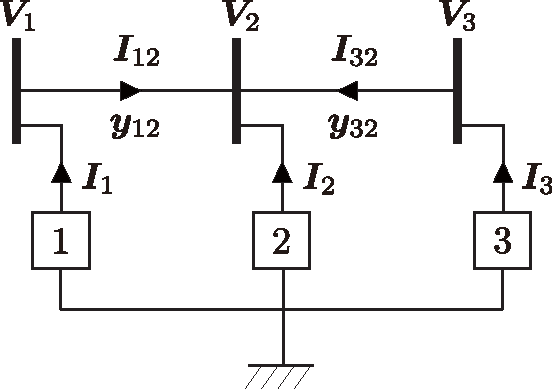
\includegraphics[width = .30\linewidth]{figs/3busex}
\caption{3つの発電機からなる電力系統モデル\red{(要変更)}}
\label{fig:3genex}
\end{figure}

\begin{figure}[t]
  \centering
  {
  \begin{minipage}{0.32\linewidth}
    \centering
    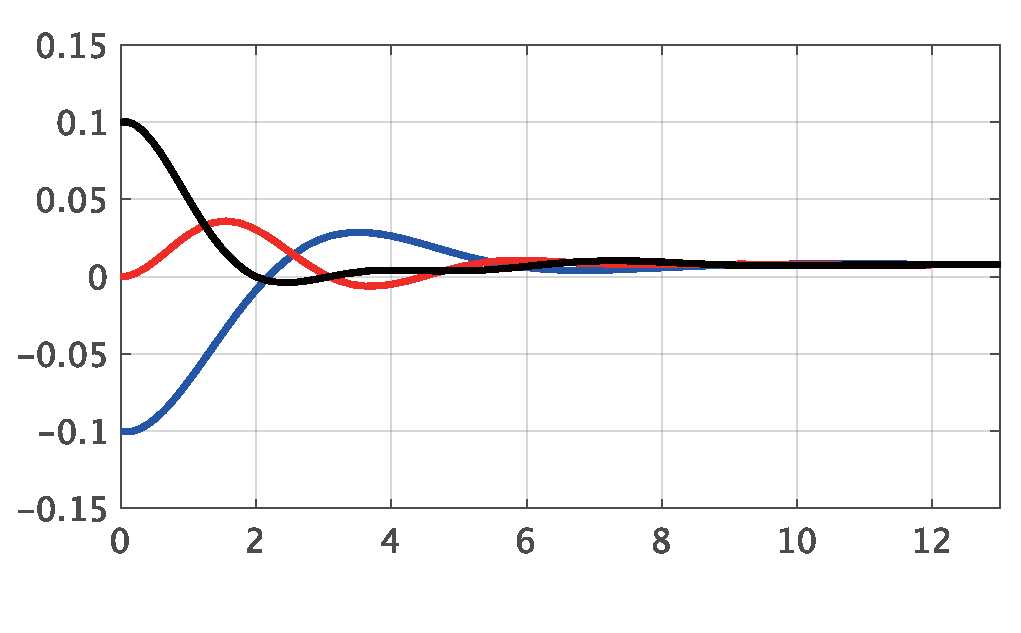
\includegraphics[width = .99\linewidth]{figs/delta}
    \subcaption{ $\delta^{\rm lin}$ }
  \end{minipage}
  \begin{minipage}{0.32\linewidth}
    \centering
    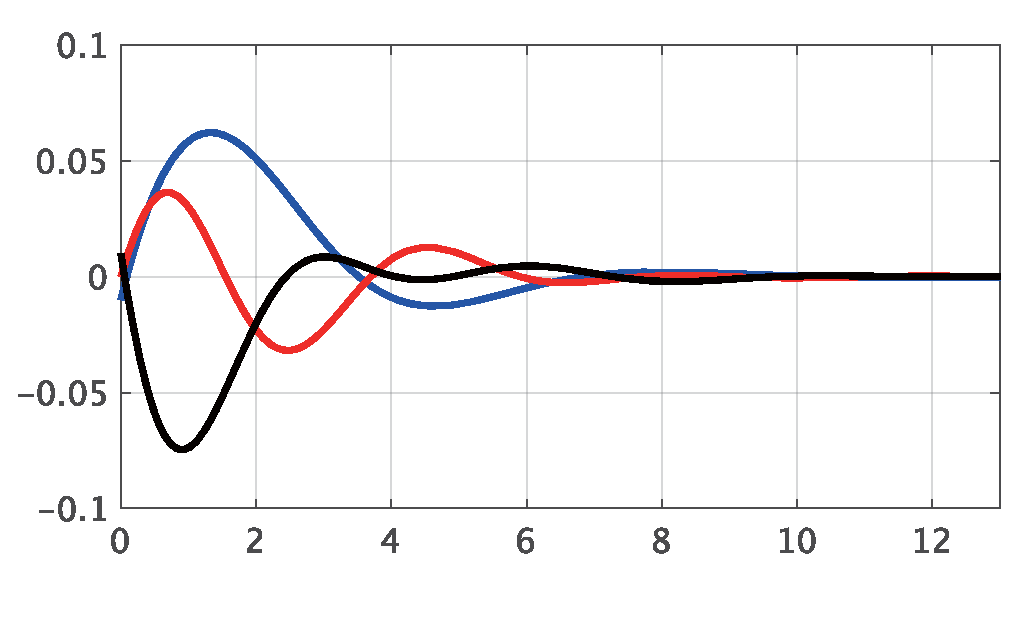
\includegraphics[width = .99\linewidth]{figs/omega}
    \subcaption{ $\Delta \omega^{\rm lin}$ }
  \end{minipage}
  \begin{minipage}{0.32\linewidth}
    \centering
    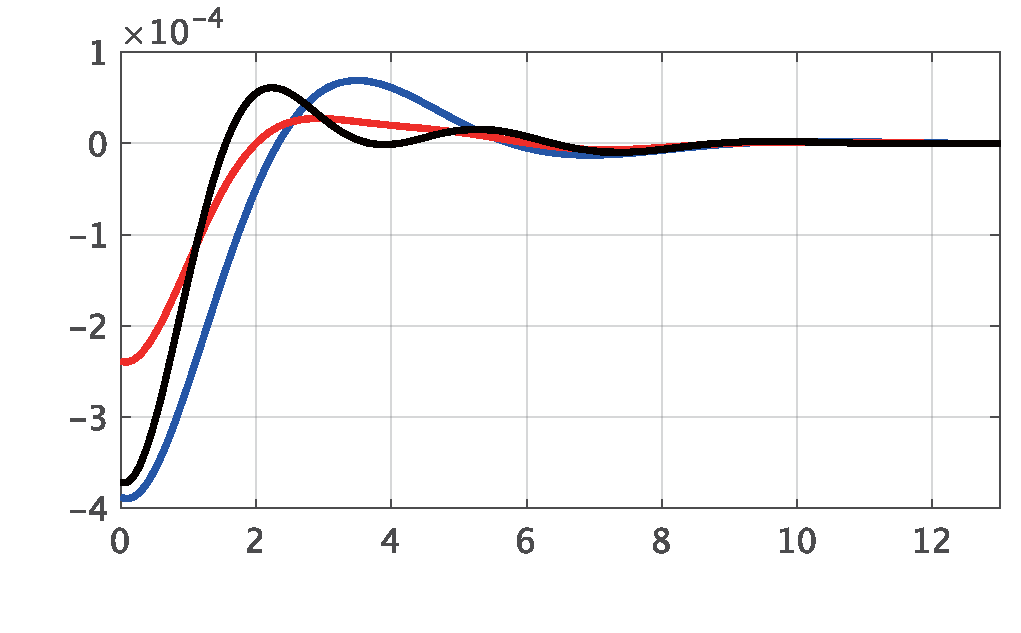
\includegraphics[width = .99\linewidth]{figs/E}
    \subcaption{ $E^{\rm lin}$ }
  \end{minipage}
  }
  \caption{近似線形モデルの初期値応答(青:発電機1,赤:発電機2,黒:発電機3)}
  \label{fig:timeex}
\end{figure}

%\begin{figure}[t!]
%\centering
%{    
%    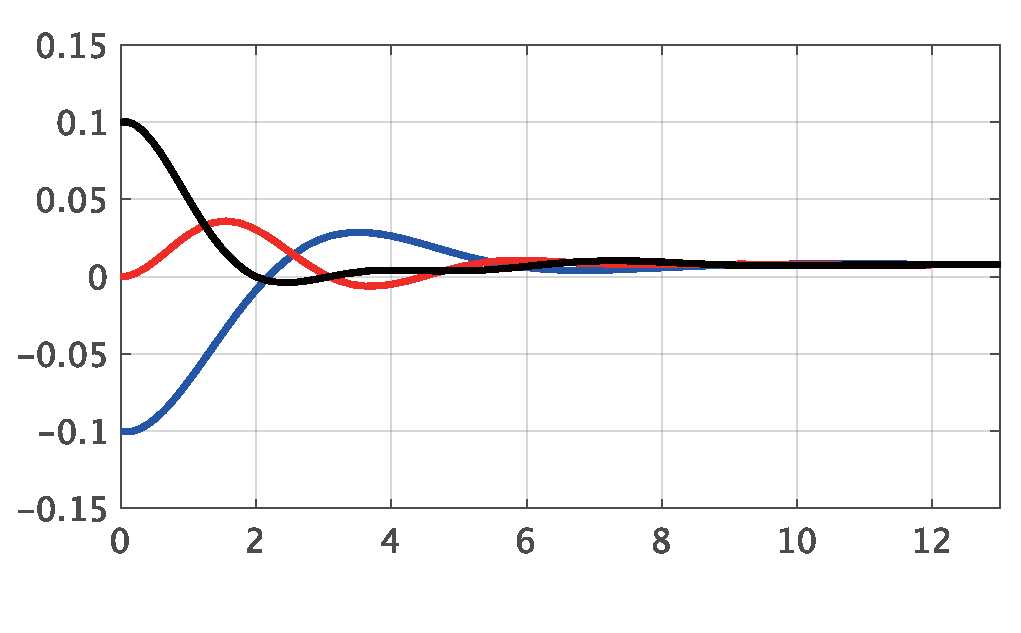
\includegraphics[width = .5\linewidth]{figs/delta}
%    \subcaption{ $\delta^{\rm lin}$ }
%    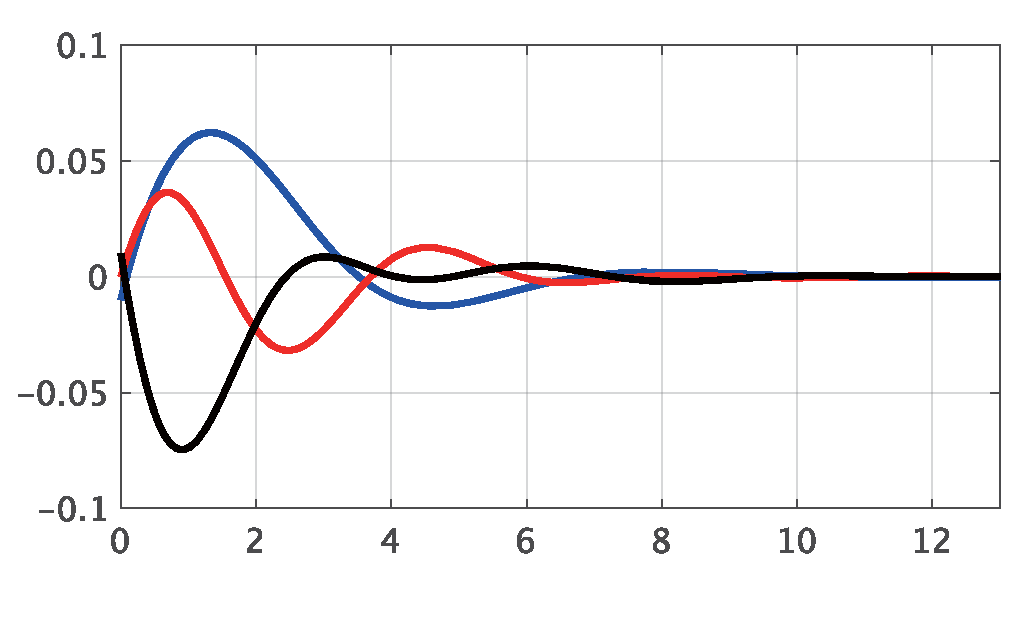
\includegraphics[width = .5\linewidth]{figs/omega}
%    \subcaption{ $\Delta \omega^{\rm lin}$ }
%    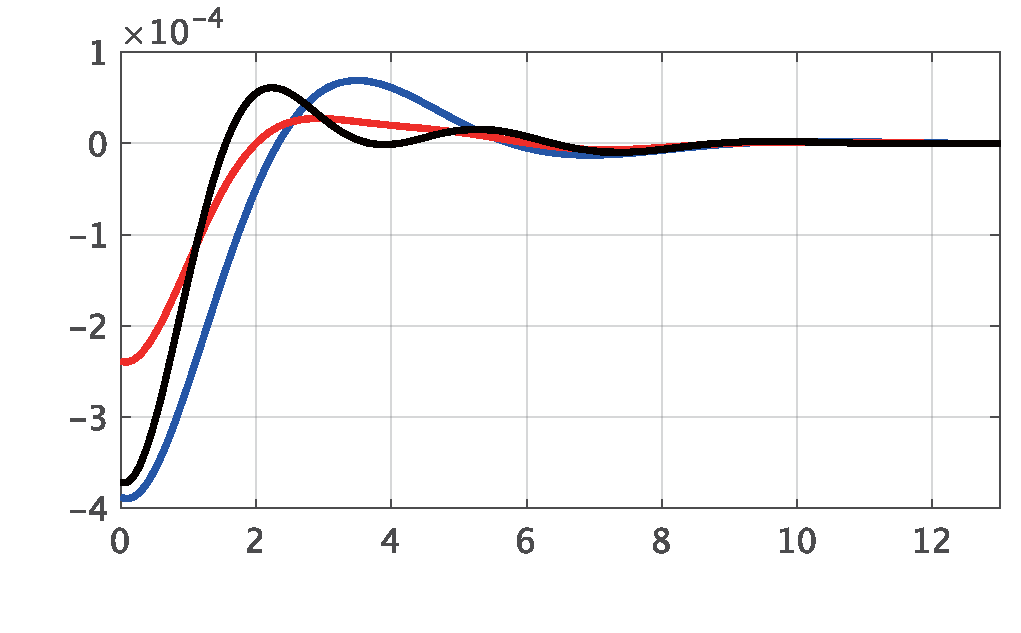
\includegraphics[width = .5\linewidth]{figs/E}
%    \subcaption{ $E^{\rm lin}$ }
%}
%\caption{近似線形モデルの初期値応答(青:発電機1,赤:発電機2,黒:発電機3)}
%\label{fig:timeex}
%\end{figure}

\begin{figure}[t]
  \centering
  {
  \begin{minipage}{0.32\linewidth}
    \centering
    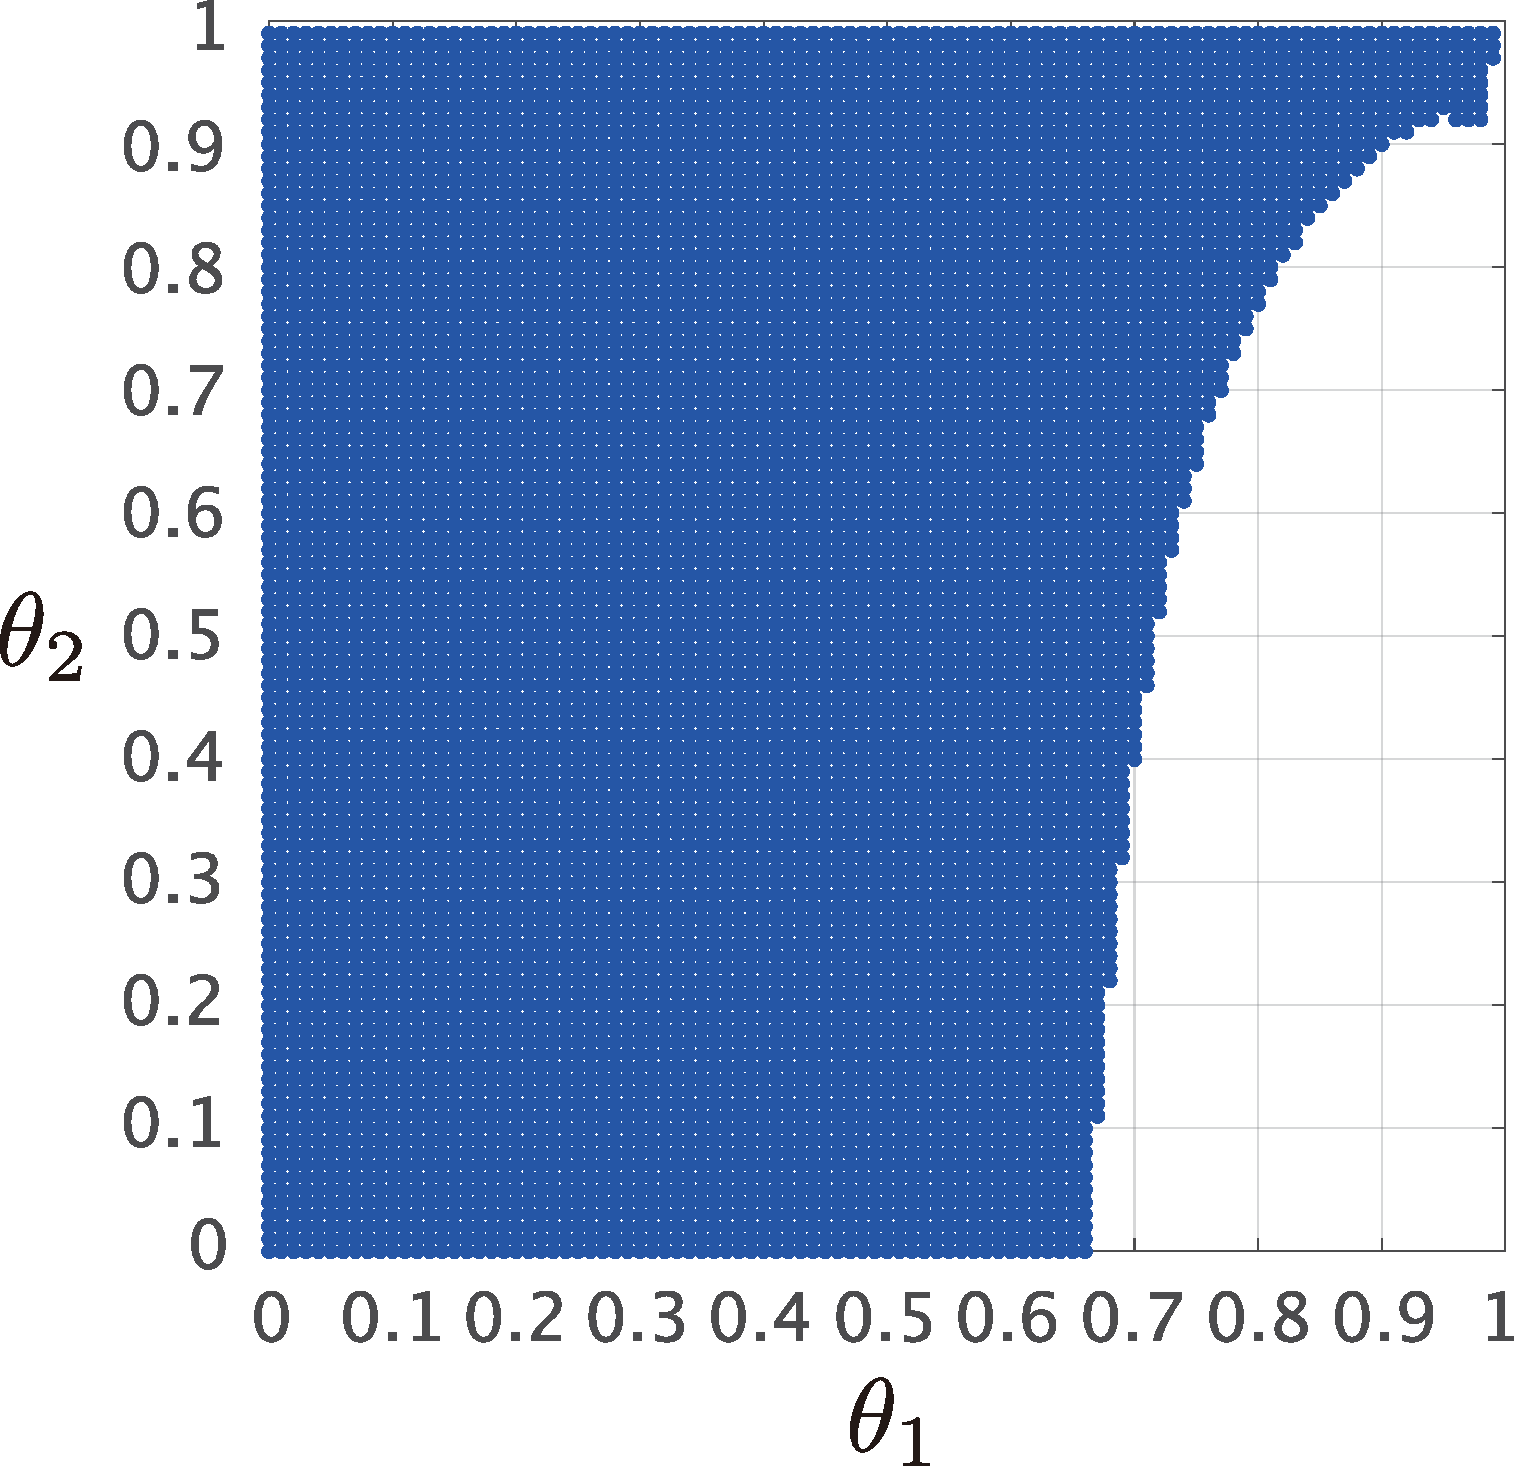
\includegraphics[width = .85\linewidth]{figs/gam01}
    \subcaption{ $\gamma=0.1$ }
  \end{minipage}
  \begin{minipage}{0.32\linewidth}
    \centering
    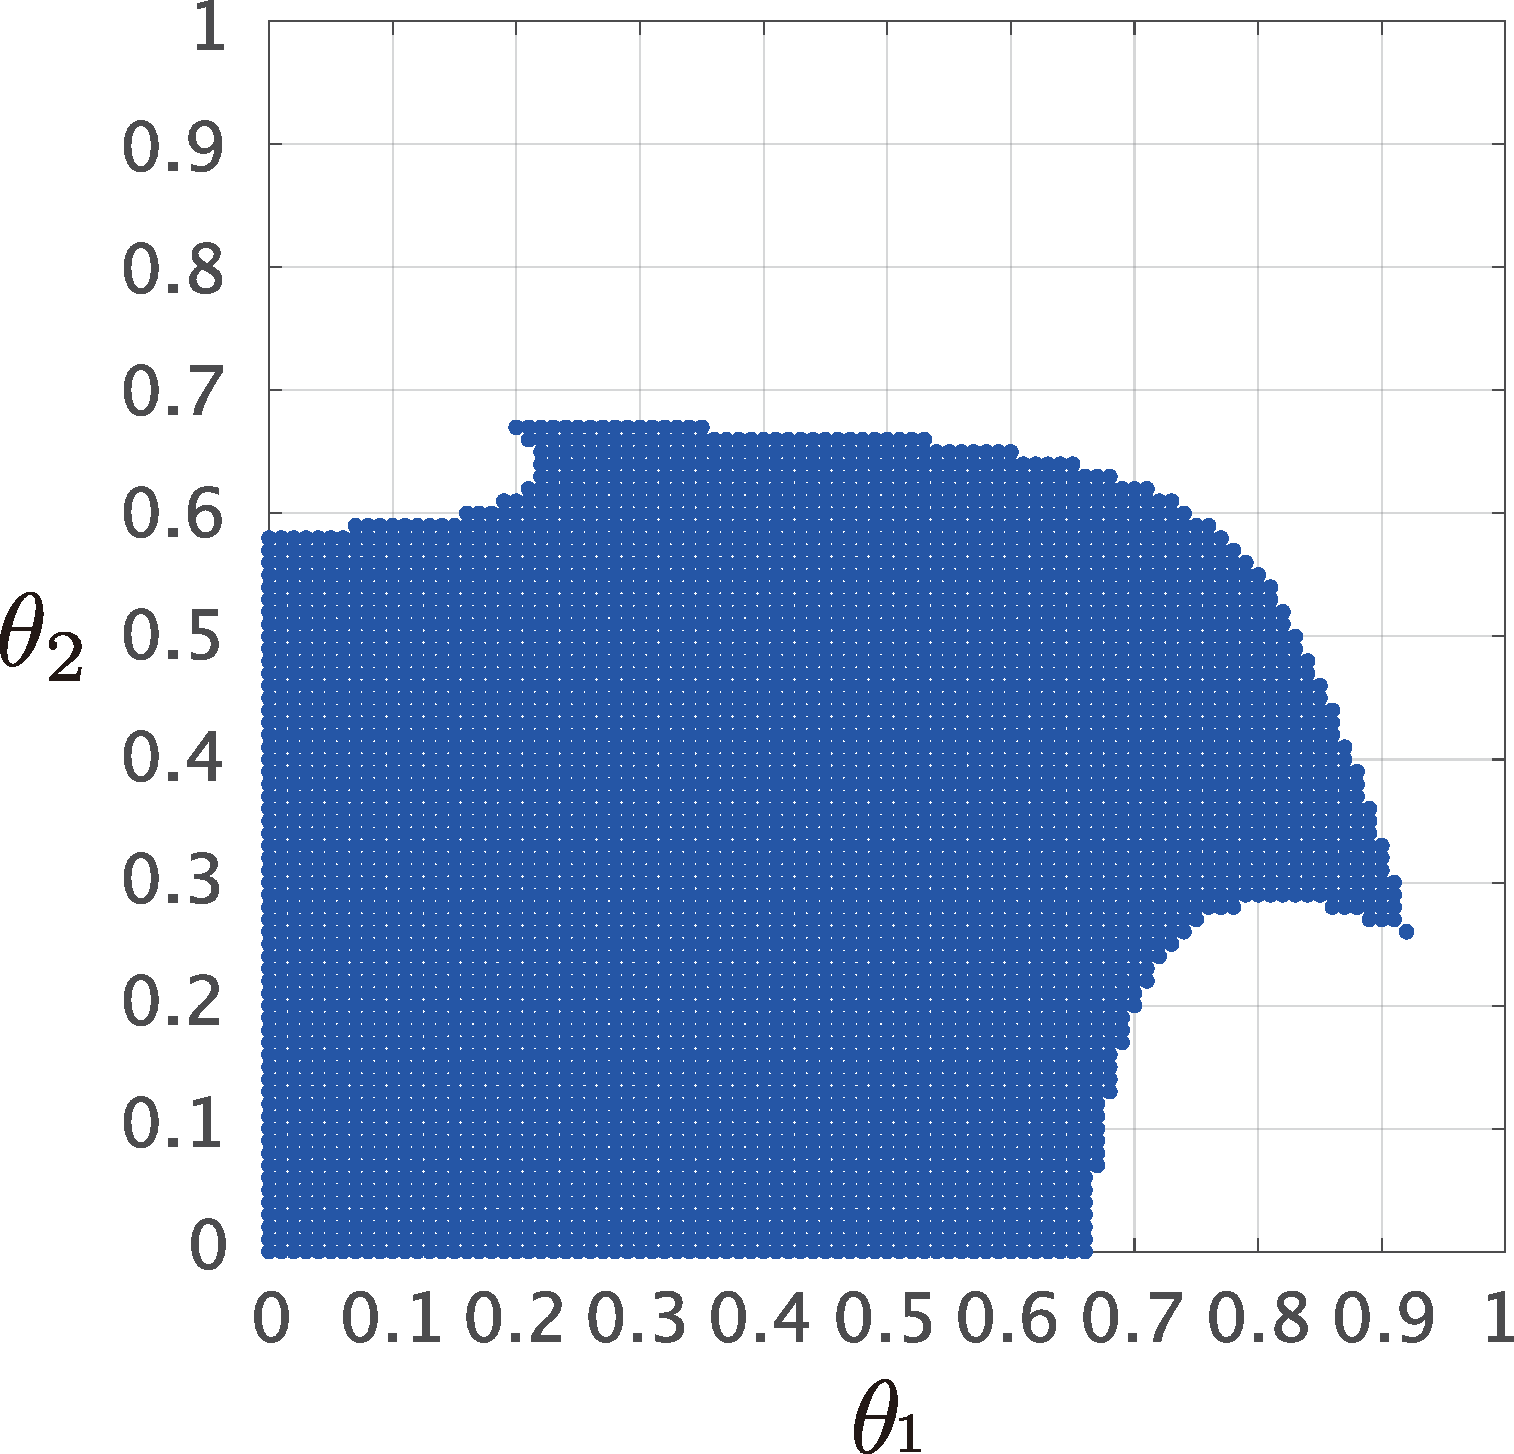
\includegraphics[width = .85\linewidth]{figs/gam2}
    \subcaption{ $\gamma=2$ }
  \end{minipage}
  \begin{minipage}{0.32\linewidth}
    \centering
    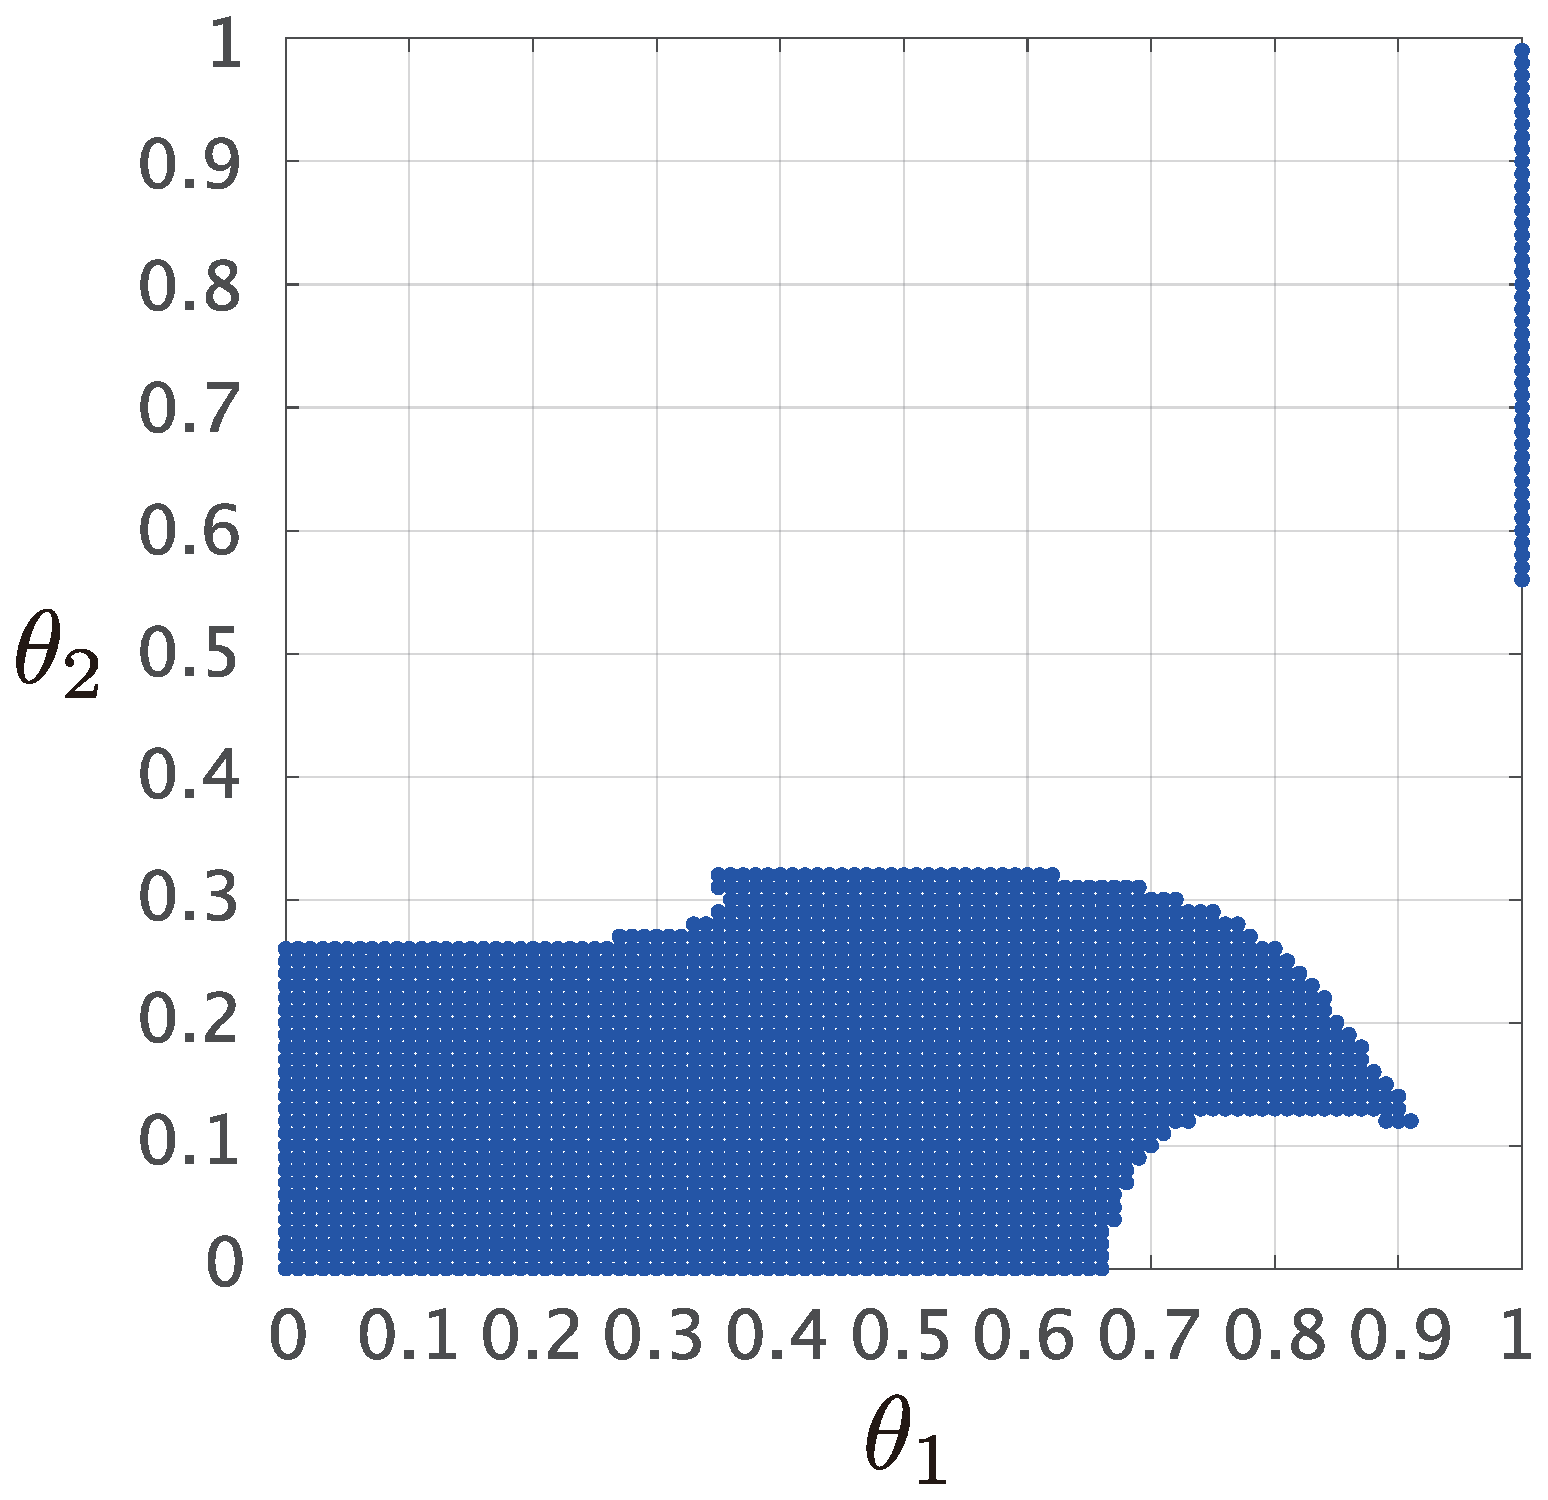
\includegraphics[width = .85\linewidth]{figs/gam5}
    \subcaption{ $\gamma=5$ }
  \end{minipage}
  \caption{近似線形モデルが安定となるパラメータの領域}
  \label{fig:gamsta}
  }
\end{figure}

\begin{例}[近似線形モデルの数値的な安定性解析]\label{ex:linsyssim}
\ref{fig:3genex}に示される3つの発電機で構成される電力系統モデルを考える。
以下では,発電機の物理定数は共通であるものとして,すべての$i \in \{1,2,3\}$に対して
\begin{align*}
M_i=1
,\qquad
D_i=1
,\qquad
\tau_{{\rm d}i} = 0.01
,\qquad
X_{{\rm d}i} = 1.01
,\qquad
X_{{\rm q}i} = 1
\end{align*}
に設定する。
また,系統周波数は$\omega_0=1$とする。

式\ref{eq:lindynu0}の近似線形モデルを導出するため,内部状態の定常値
$(\delta^{\star},E^{\star})$を設定する。
内部電圧の定常値は各発電機で異なる値として
\begin{subequations}\label{eq:exEsds}
\begin{align}
E^{\star}_1=1
,\qquad
E^{\star}_2=2
,\qquad
E^{\star}_3=3
\end{align}
に設定する。
回転子偏角差の定常値は,パラメータ$\theta_1 \in [0, 1]$を用いて
\begin{align}
\delta_{12}^{\star}= - \frac{\pi}{2} \theta_1
,\qquad
\delta_{13}^{\star}=  \frac{\pi}{2} \theta_1
\end{align}
と表す。
\end{subequations}
パラメータ$\theta_1$の大きさは,定常状態における回転子偏角差の大きさに対応している。
このパラメータの変化は,式\ref{eq:sysmats}のシステム行列の変化として近似線形モデルに現れる。
送電網のアドミタンス行列も同様に,2つのパラメータ$\gamma >0$と$\theta_2 \in [0,1]$を用いて
\begin{align*}
\bm{Y} =
\theta_2
\mat{
\gamma & 0 & 0 \\
0 &\gamma & 0 \\
0 & 0 & \gamma
}
 +
\bm{j} (1-\theta_2) 
\mat{
-1 & 1 & 0 \\
1 & -2 & 1 \\
0 & 1 & -1 
}
\end{align*}
と表す。
ここで,$\gamma$はアドミタンス行列の実部の絶対値を指定するパラメータであり,$\theta_2$は実部と虚部の相対的な大小関係を指定するパラメータである。
アドミタンス行列のパラメータ変化は,式\ref{eq:defkh}の縮約コンダクタンス$B^{\rm red}_{ij}$と縮約サセプタンス$G^{\rm red}_{ij}$の値の変化として近似線形モデルに現れる。
上記のパラメータ$(\gamma,\theta_1,\theta_2)$を変化させて,近似線形モデルの安定性を数値的に解析する。

まず,$\gamma=2$,$\theta_1=0.3$,$\theta_2=0.2$とした場合のシステムの初期値応答を確認してみよう。
適当な初期値を設定した場合の結果を\ref{fig:timeex}に示す。
この図から,このパラメータ設定の場合には,式\ref{eq:linmconv}のように発電機群の内部状態が収束していることがわかる。

つぎに,(a) $\gamma=0.1$,(b) $\gamma=2$,(c) $\gamma=5$に設定する。
この(a)--(c)の場合において,$\theta_1$と$\theta_2$を0.01の刻み幅で変化させて式\ref{eq:lindynu0}の$\Psi$の固有値を調べることにより,近似線形モデルが安定であるか否かを網羅的に確認してみよう。
\ref{fig:gamsta}にその結果を示す。
近似線形モデルが安定となったパラメータを青の領域で表している。
\ref{fig:gamsta}(a)--(c)から,$\gamma$が大きくなる,すなわち,アドミタンス行列の実部であるコンダクタンス行列の絶対値が大きくなるにしたがって,近似線形モデルが安定となるパラメータの領域が狭くなっていることがわかる。

また,どの図においても原点付近のパラメータ領域,すなわち,定常状態における回転子偏角差が小さく,かつ,アドミタンス行列の実部が虚部よりも相対的に小さい場合には,近似線形モデルが安定であることがわかる。
なお,$\gamma=5$,$\theta_1=1$,$\theta_2 \in [0.56,0.99]$のパラメータでは,挙動は非常に振動的であるが,例外的に安定であった。
これらの結果から,定常状態における回転子偏角差が小さく,コンダクタンス行列がサセプタンス行列よりも相対的に小さい場合に,近似線形モデルが安定になりやすい傾向にあることがわかる。
\end{例}




\subsection{近似線形モデルの数学的な安定性解析\advanced}

\subsubsection{近似線形モデルの安定性と同期}

本節では,式\ref{eq:lindyn}の近似線形モデルの安定性を数学的に解析する。
その安定性は,式\ref{eq:lindynu0}の行列$\Psi$の固有値により特徴づけられる。
第\ref{sec:numlinsta}節で議論されているように,$\Psi$は正則ではなく,
\begin{align}\label{eq:eqset}
\mathcal{M} =
 \sfspan\left\{
 \mat{
 \mathds{1}\\
 0\\
 0
 }
 \right\}
\end{align}
は$\Psi$の零固有値に対する固有空間である。
この集合は,相対的な値を一定に保ってすべての発電機の偏角を変化させた等価な定常値の集合を表している。
したがって,近似線形モデルの状態が式\ref{eq:eqset}の平衡点集合のうちのどの点に収束するかは問題とならない。
この事実に基づき,つぎの定義を与える。

\begin{定義}[近似線形モデルの同期]
\label{def:stalin}
式\ref{eq:lindyn}の近似線形モデルを考える。
任意の初期値に対して,内部状態が式\ref{eq:eqset}の平衡点集合$\mathcal{M}$のいずれかの点に収束するとき,近似線形モデルは\emph{同期する}と呼ぶ。
ただし,入力は恒等的に0とする。
\end{定義}

定義\ref{def:stalin}における同期は,任意の初期値に対して,式\ref{eq:linmconv}が成り立つことを表している。
なお,式\ref{eq:linmconv}において$c_0$の値は任意であるため,その任意性を「$\mathcal{M}$のいずれかの点に収束すること」として表現している。

以下では,式\ref{eq:lindynu0}の$\Psi$の核空間が1次元であること,すなわち,
\[
\sfker \Psi = \mathcal{M}
\]
であることを仮定する。
これは近似線形モデルの同期が達成されるための必要条件である。
特に,$A$が正則である場合には,
\begin{align}\label{eq:nescon}
\sfker (L-CA^{-1}B) = \sfspan
\left\{
\mathds{1}
\right\}
\end{align}
と等価であることが示される。


\subsubsection{偏差サブシステムの漸近安定性}

式\ref{eq:lindyn}の近似線形モデルが同期することの必要十分条件は,式\ref{eq:lindynu0}の行列$\Psi$について,零固有値を除くすべての固有値の実部が負であることである。
以下の議論のため,つぎの2つの用語を定義しておく。

\begin{定義}[正方行列の安定性]
\label{def:matsta}
正方行列$A$に対して,そのすべての固有値の実部が負であるとき,$A$は\emph{安定}であると呼ぶ。
\end{定義}

\begin{定義}[線形システムの漸近安定性]
\label{def:difsta}
線形の微分方程式で記述される
\begin{align}\label{eq:difAB}
\dot{x}(t)=Ax(t) +Bu(t)
\end{align}
に対して,行列$A$が安定であるとき,式\ref{eq:difAB}の線形システムは\emph{漸近安定}であると呼ぶ。
\end{定義}

式\ref{eq:lindynu0}の行列$\Psi$は零固有値をもつため,定義\ref{def:matsta}の意味で安定ではないことに注意されたい。
式\ref{eq:lindyn}の近似線形モデルの同期を解析するために,零固有値に対応する不変な固有空間を取り除くことを考えよう。
具体的には,式\ref{eq:lindyn}の$3N$次元の微分方程式から1次元の不変部分空間を除いた$(3N-1)$次元のサブシステムを求める。
この$(3N-1)$次元のサブシステムを\emph{偏差サブシステム}と呼ぶ。
以下では,偏差サブシステムが漸近安定であることが,式\ref{eq:lindyn}の近似線形モデルが同期することの必要十分条件となることを確認する。

式\ref{eq:lindyn}の状態$\delta^{\rm lin}$に対して基底変換を適用することにより,偏差サブシステムを導出することを考える。
このために,$\delta^{\rm lin}$の不変な成分に対応する,式\ref{eq:eqset}の固有空間$\mathcal{M}$は,式\ref{eq:LBker}に示されている$L$と$B$の共通の核空間に由来することに注目する。
この共通の核空間が存在することは,
\begin{align}\label{eq:sfkerW}
\sfker W = \sfspan\{ \mathds{1}\}
\end{align}
を満たす任意の行列$W \in \mathbb{R}^{(N-1)\times N}$を用いて
\begin{align}\label{eq:decLB}
L = L_0 W 
,\qquad
B = B_0 W 
\end{align}
と分解できることを意味している。
この事実を具体例で確認してみよう。

\begin{例}[同一の核空間をもつ行列による分解]\label{ex:Ldec}
式\ref{eq:sysmats}の$L$について,$N=3$である場合を考えてみよう。
このとき,$L$は
\begin{align*}
L=
\mat{
L_{12}+L_{13} & -L_{12} & -L_{13}\\
-L_{21}& L_{21} + L_{23} & -L_{23}\\
- L_{31}& -L_{32} & L_{31}+L_{32}
}
\end{align*}
と表せる。
ただし,$L_{ij}:= E_i^* E_j^* k_{ij}(\delta_{ij}^*)$である。
これに対して,式\ref{eq:sfkerW}を満たす行列,すなわち,$W \mathds{1}=0$を満たす行フルランクな行列の例として
\begin{align*}
W=\mat{
1 & -1 & 0 \\
0 & 1 & -1
}
\end{align*}
を考える。
この$W$を用いる場合には,$L$は
\begin{align*}
L = \underbrace{
\mat{
L_{12} + L_{13} & L_{13} \\
-L_{21}& L_{23} \\
-L_{31} & -(L_{31}+L_{32})
}
}_{L_0}
W
\end{align*}
のように分解できる。
一般に,$W$の$WW^{\dagger}=I$となる適当な右逆行列$W^{\dagger}$を用いれば,$L_0$は$LW^{\dagger}$として求められる。
この例の場合では,その右逆行列は
\begin{align*}
W^{\dagger} = \mat{
1 & 1\\
0 & 1\\
0 & 0
}
,\qquad
W^{\dagger} = \mat{
1 & 2\\
0 & 2\\
0 & 1
}
\end{align*}
などのように選ぶことができる。
このように,$W^{\dagger}$は一意ではないが,$WW^{\dagger}=I$であれば,いかなる$W^{\dagger}$に対しても結果は等しい。
なお,式\ref{eq:sysmats}の$B$も$L$と同様の構造をもつため,共通の$W$を用いて分解することが可能である。
\end{例}

式\ref{eq:sfkerW}を満たす適当な行列$W \in \mathbb{R}^{(N-1)\times N}$を用いて,式\ref{eq:lindyn}の$\delta^{\rm lin}$に関する基底変換として
\begin{align}\label{eq:delbt}
\delta^{\rm lin}_{\rm e}  := W \delta^{\rm lin}
,\qquad
\overline{\delta}^{\rm lin}_{\rm e} :=
\frac{1}{N} \mathds{1}^{\sf T}
\delta^{\rm lin}
\end{align}
を定義する。
このとき
\begin{align*}
\mat{
W \\
\frac{1}{N} \mathds{1}^{\sf T}
}^{-1}
= \mat{
W^{\dagger}& \mathds{1}
}
\end{align*}
が満たされるように$W^{\dagger}$を定義することができる。
これは
\begin{align*}
\mat{
W \\
\frac{1}{N} \mathds{1}^{\sf T}
}
\mat{
W^{\dagger}& \mathds{1}
}
=\mat{
WW^{\dagger} & W \mathds{1}\\
\frac{1}{N} \mathds{1}^{\sf T} W^{\dagger} & \frac{1}{N} \mathds{1}^{\sf T} \mathds{1}
}
=\mat{
I & 0\\
0 & 1
}
\end{align*}
において$\frac{1}{N} \mathds{1}^{\sf T}W^{\dagger}=0$であるような$W^{\dagger}$を選ぶことに等しい。
このように定義すると,式\ref{eq:delbt}の基底変換に対する逆変換は
\begin{align}\label{eq:batrinv}
\delta^{\rm lin}
=
W^{\dagger}
\delta^{\rm lin}_{\rm e} +
\mathds{1}
\overline{\delta}^{\rm lin}_{\rm e}
\end{align}
と表せる。
ここで,$\mathds{1}$は$\delta^{\rm lin}$の共通成分を表す基底であり,$W^{\dagger}$はそれ以外の偏差成分を表す基底である。
すなわち,$\delta^{\rm lin}$の共通成分が$\overline{\delta}^{\rm lin}_{\rm e}$であり,偏差成分が$\delta^{\rm lin}_{\rm e}$である。
この基底変換を式\ref{eq:lindyn}の近似線形モデルに行うと
\begin{align}\label{eq:lindynnew}
\mat{
\dot{\overline{\delta}}^{\rm lin}_{\rm e} \\
\dot{\delta}^{\rm lin}_{\rm e} \\
M \Delta \dot{\omega}^{\rm lin} \\
\tau_{{\rm d}} \dot{E}^{\rm lin}
}
&=
\mat{
0 & 0 & \frac{\omega_0}{N} \mathds{1}^{\sf T} & 0 \\
0& 0 & \omega_0 W & 0\\
0&  -L_0 & -D & -C \\
0 & B_0 & 0 & A
 }
\mat{
\overline{\delta}^{\rm lin}_{\rm e} \\
\delta^{\rm lin}_{\rm e} \\
\Delta \omega^{\rm lin}\\
 E^{\rm lin}
}
+
\mat{
0 & 0 \\
0 & 0 \\
I & 0 \\
0 & I \\
}
\mat{
P_{{\rm mech}}^{\rm lin} \\
V_{{\rm field}}^{\rm lin}
}
\end{align}
が得られる。
ただし,$L_0 = L W^{\dagger}$,$B_0 = B W^{\dagger}$である。
この表現において,1つ目の状態として現れているスカラの状態変数$\overline{\delta}^{\rm lin}_{\rm e}$に注目しよう。
この状態変数は,その他の状態変数である
$(\delta^{\rm lin}_{\rm e},\Delta \omega^{\rm lin}, E^{\rm lin})$には影響を及ぼさない。
したがって,その冗長な状態変数$\overline{\delta}^{\rm lin}_{\rm e}$を削除して得られる
\begin{align}\label{eq:lindynred}
\mat{
\dot{\delta}^{\rm lin}_{\rm e} \\
M \Delta \dot{\omega}^{\rm lin} \\
\tau_{{\rm d}} \dot{E}^{\rm lin}
}
&=
\mat{
 0 & \omega_0 W & 0\\
  -L_0 & -D & -C \\
 B_0 & 0 & A
 }
\mat{
\delta^{\rm lin}_{\rm e} \\
\Delta \omega^{\rm lin}\\
 E^{\rm lin}
}
+
\mat{
0 & 0 \\
I & 0 \\
0 & I \\
}
\mat{
P_{{\rm mech}}^{\rm lin} \\
V_{{\rm field}}^{\rm lin}
}
\end{align}
は,式\ref{eq:lindynnew}の状態変数$(\delta^{\rm lin}_{\rm e},\Delta \omega^{\rm lin}, E^{\rm lin})$の挙動を厳密に再現する低次元なサブシステムとなる。
これが$(3N-1)$次元の偏差サブシステムを記述する状態方程式である。

式\ref{eq:lindynred}の偏差サブシステムが漸近安定であること,すなわち,任意の初期値に対して
\[
\lim_{t\rightarrow \infty}\delta^{\rm lin}_{\rm e}(t)= 0 ,\qquad
\lim_{t\rightarrow \infty}\Delta \omega^{\rm lin}(t)=0 ,\qquad
\lim_{t\rightarrow \infty} E^{\rm lin}(t)=0
\]
が成り立つことが示されれば,式\ref{eq:batrinv}の関係から,式\ref{eq:linmconv}が成り立つことが示される。
ただし,
\[
c_0=
\lim_{t\rightarrow \infty} \overline{\delta}^{\rm lin}_{\rm e}(t) 
\]
である。
以上の議論から,式\ref{eq:lindynred}の偏差サブシステムが漸近安定であることは,式\ref{eq:lindyn}の近似線形モデルが同期することの必要十分条件であることがわかる。


\subsubsection{偏差サブシステムの漸近安定性}



,すわなち,
\begin{align*}
\mat{
I &0&0 \\
0&\sfdiag(M_i) & 0 \\
0&0 &\sfdiag(\tau_{{\rm d}i}) 
}^{-1}
\mat{
 0 & \omega_0 W & 0\\
  -L_0 & -\sfdiag(D_i) & -C \\
 B_0 & 0 & A
 }
\end{align*}
が安定であることを示すためには,式\ref{eq:trFs}の$F(s)$と式\ref{eq:trGseq}右辺の$G(s)$から構成される$(3N-1)$次元のフィードバック系が内部安定であることを示せば良い。
特に,式\ref{eq:trGseq}の右辺と左辺は$s$の関数としては等しいことから,左辺の伝達関数が正実であるならば右辺の伝達関数も正実である。
以上の事実から,$G(s)$の表現形式にかからわずその正実性が示されるのであれば,式\ref{eq:lindyn}の線形近似システムが同期することを結論づけられる。
なお,式\ref{eq:lindynu0}の$\Psi$の核空間が1次元,すなわち,式\ref{eq:eqset}の$\mathcal{M}$に等しい限りは,$G(s)$の内部で2つ以上の積分器が相殺されることはない。

%%%%%%%%%%%%%



式\ref{eq:decLB}の分解を用いて,ラプラス領域における\eqref{eq:trGs}の$G(s)$の変形として
\begin{align}\label{eq:trGseq}
\spliteq{
& - \frac{1}{s} I \cdot
\underbrace{
\left\{ -C \bigl( \sfdiag(\tau_{{\rm d}i})s -A \bigr)^{-1} B - L \right\}
}_{H(s)}
\\
& \hspace{8em}=
- 
\underbrace{
\left\{ -C \bigl( \sfdiag(\tau_{{\rm d}i})s -A \bigr)^{-1} B_0 - L_0 \right\} 
}_{H_0(s)}
\cdot
\frac{1}{s} W
}
\end{align}
を考える。
ラプラス領域においてこの等式は「自明な」ものであるが,時間領域における$G(s)$の実現を考える場合には異なる解釈が与えられる。
具体的には,$G(s)$への入力を$u_g(s)$とすると,式\ref{eq:trGseq}の左辺は,$u_g(s)$を伝達関数$H(s)$に作用させて出てきた信号を$\frac{1}{s}$で積分するものと解釈できる。
一方で,右辺は$W u_g(s)$という信号を$\frac{1}{s}$で積分した後で$H_0(s)$に作用させるものと解釈できる。

式\ref{eq:trGseq}の変形で重要な点は,「積分器の数が両辺で異なる」という事実である。
具体的には,左辺では$H(s) u_g(s)$という$N$次元の信号を各要素で並列に積分するため,積分器は$N$個存在するのに対して,右辺では$W u_g(s)$という$(N-1)$次元の信号の積分であるため,積分器は$(N-1)$個しか存在していない。
これは,右辺の表現では$G(s)$の入出力関係に影響しない冗長な積分器が削除されていることを意味している。
この冗長な積分器は$L$や$B$の共通の核空間に由来するものであることに注意されたい。


\begin{figure}[t]
\centering
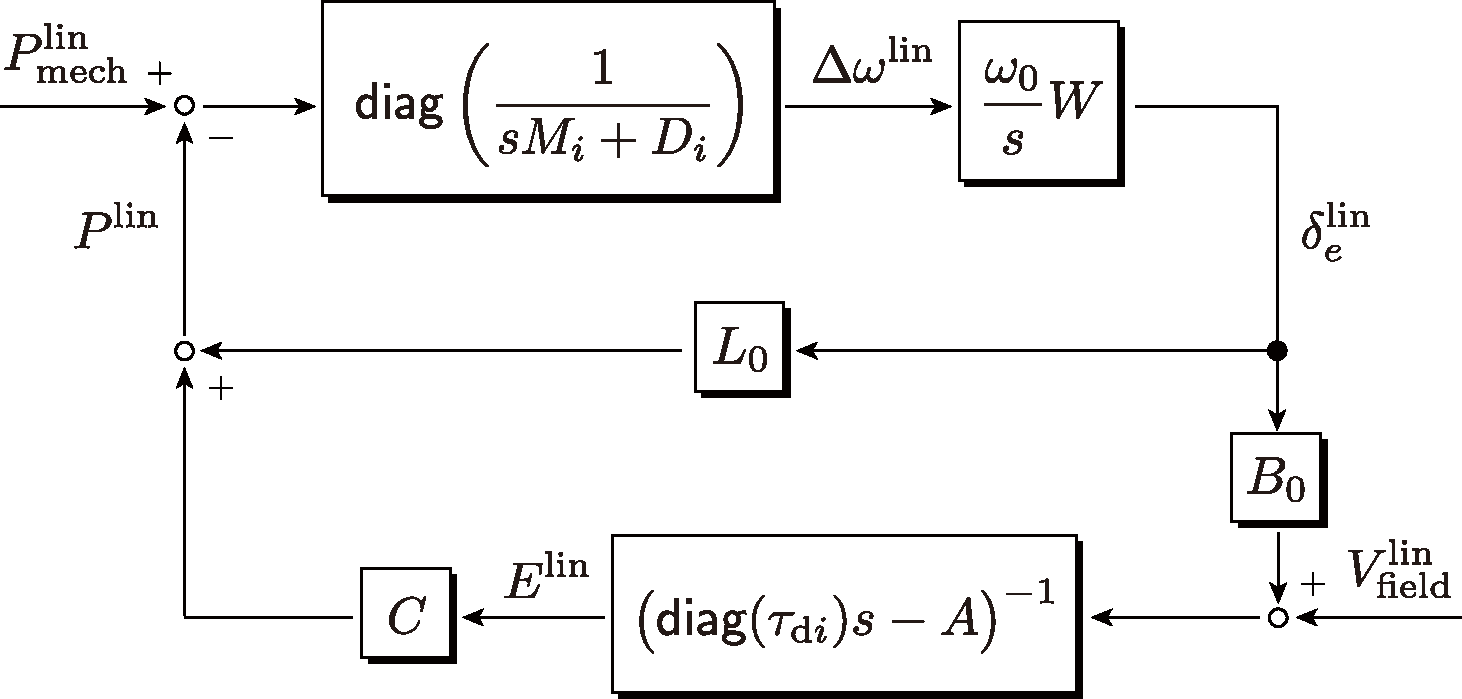
\includegraphics[width = .75\linewidth]{figs/blocklinsysnew}
\caption{冗長な積分器が取り除かれた偏差サブシステムのブロック線図表現}
\label{fig:blocklinnew}
\end{figure}

式\ref{eq:trGseq}右辺の表現によれば,\ref{fig:blocklin}のフィードバック系を\ref{fig:blocklinnew}のように変形することができる。
この図の右上に位置する$\delta^{\rm lin}_{\rm e}$は,$N$次元の$\delta^{\rm lin}$から不変な固有空間の成分を削除した$(N-1)$次元の偏差成分を表している。
より正確にはつぎのように説明できる。






\subsubsection{近似線形モデルの伝達関数表現}

システム制御理論における伝達関数の正実性やそれに類する概念に基づいて,式\ref{eq:lindyn}の近似線形モデルの同期を解析することを考えよう。
まず,時間領域における式\ref{eq:lindyn}の微分方程式をラプラス変換して,ラプラス領域(周波数領域)におけるシステム表現を導出する。
\ref{fig:blocklin}は式\ref{eq:lindyn}をラプラス変換して得られるブロック線図である。
この図は以下の手順により導出できる。
いま,3行目の$E^{\rm lin}$に関する微分方程式に注目すると,そのラプラス変換は
\begin{align*}
s \sfdiag(\tau_{{\rm d}i}) E^{\rm lin}(s)
= B \delta^{\rm lin}(s) + A E^{\rm lin}(s) + V^{\rm lin}_{\rm field}(s)
\end{align*}
と得られる。
ただし,ラプラス領域の変数も時間領域の変数と同じ記号を用いて表している。
これを$E^{\rm lin}(s)$に関して解けば
\begin{align*}
E^{\rm lin}(s) = \bigl( \sfdiag(\tau_{{\rm d}i})s -A \bigr)^{-1} 
\left\{ B \delta^{\rm lin}(s)
+ V^{\rm lin}_{\rm field}(s) \right\}
\end{align*}
が得られる。
これは\ref{fig:blocklin}の最下段にある右と中央のブロックに相当する。
同様に,式\ref{eq:lindyn}の1行目と2行目の微分方程式もラプラス変換し,注目している変数に関する方程式を代数的に解くことによって,\ref{fig:blocklin}のその他のブロックも得られる。
なお,\ref{fig:blocklin}左側に位置する$P^{\rm lin}$は,各発電機バスに供給される有効電力を並べたベクトルであると解釈できる。

\begin{figure}[t]
\centering
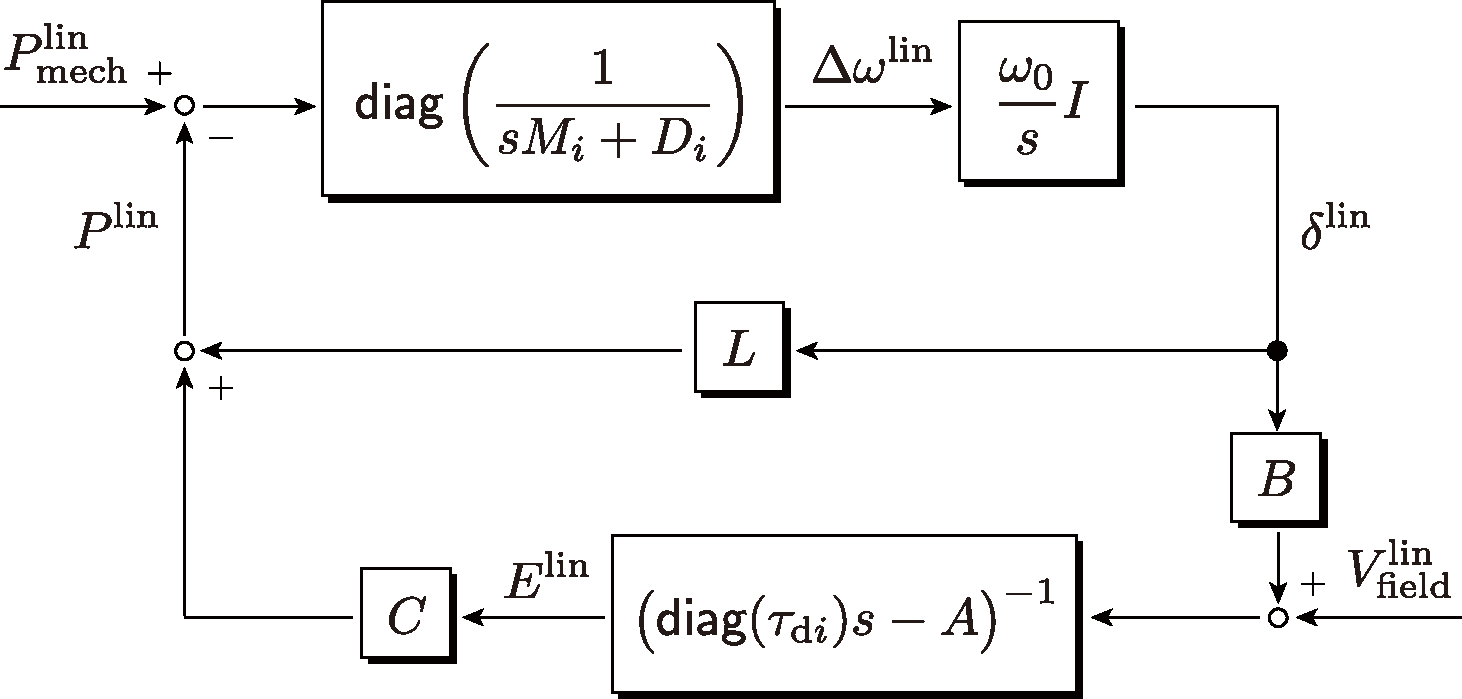
\includegraphics[width = .75\linewidth]{figs/blocklinsys2}
\caption{伝達関数に基づく近似線形モデルのブロック線図表現}
\label{fig:blocklin}
\end{figure}




つぎに,\ref{fig:blocklin}のブロック線図を解析しやすい形式に変形することを考える。
具体的には,右上の$\frac{\omega_0}{s}I$のブロックを分割し,左上のブロックと$\omega_0$の積として
%\begin{subequations}\label{eq:trFsGs}
\begin{align}\label{eq:trFs}
F(s) :=  
\sfdiag \left( 
\frac{\omega_0}{M_i s + D_i}
\right)
\end{align}
を定義する。
また,残りの$\frac{1}{s}I$の項を下側のブロックに移動させ,それらの積として
\begin{align}\label{eq:trGs}
G(s) :=  - \frac{1}{s} 
\underbrace{
\left\{ -C \bigl( \sfdiag(\tau_{{\rm d}i})s -A \bigr)^{-1} B - L \right\}
}_{H(s)}
\end{align}
%\end{subequations}
を定義する。
これにより,\ref{fig:blocklin}から入力を除いたブロック線図は,\ref{fig:staFG}(a)のように2つのシステムのネガティブ・フィードバック結合として表現できる。

\subsubsection{伝達関数の安定性と正実性}

\ref{fig:staFG}(a)による式\ref{eq:lindyn}の伝達関数表現においては,伝達関数$F(s)$は単純な1次系が並列されたシステムであるため,その性質は容易に調べられる。
例えば,$\omega_0$,$M_i$,$D_i$はすべて正の定数であることから,$F(s)$は常に安定である。
伝達関数に対する安定性はつぎのように定義される。

\begin{定義}[伝達関数の安定性]\label{def:trsta}
伝達関数$Q(s)$のすべての極の実部が負であるとき,$Q(s)$は\emph{安定}であると呼ぶ。
\end{定義}

式\ref{eq:trFs}の$F(s)$の極,すなわち,分母多項式$M_i s + D_i$の零点は$s=-\frac{D_i}{M_i}$であることから$F(s)$は安定である。
この伝達関数の極は,時間領域における状態空間実現\red{(付録??)}である
\begin{align}\label{eq:Fss}
F: \simode{
\dot{x}_f &= \textstyle - \sfdiag \left( 
\frac{D_i}{ M_i} 
\right)
x_f
+
\sfdiag \left( 
\frac{1}{ M_i} 
\right)
u_f \\
y_f &= \omega_0 x_f
}
\end{align}
に対するシステム行列の固有値と一致する。
なお,$F(s)$の微分方程式による実現は,座標変換の自由度があるため唯一ではないが,その固有値は実現に依らず不変である。

さらに,式\ref{eq:trFs}の$F(s)$は正実性(positive realness)と呼ばれる特性をもつ。
伝達関数に対する正実性はつぎのように定義される。

\begin{figure}[t]
  \centering
  {
  \begin{minipage}{0.49\linewidth}
    \centering
    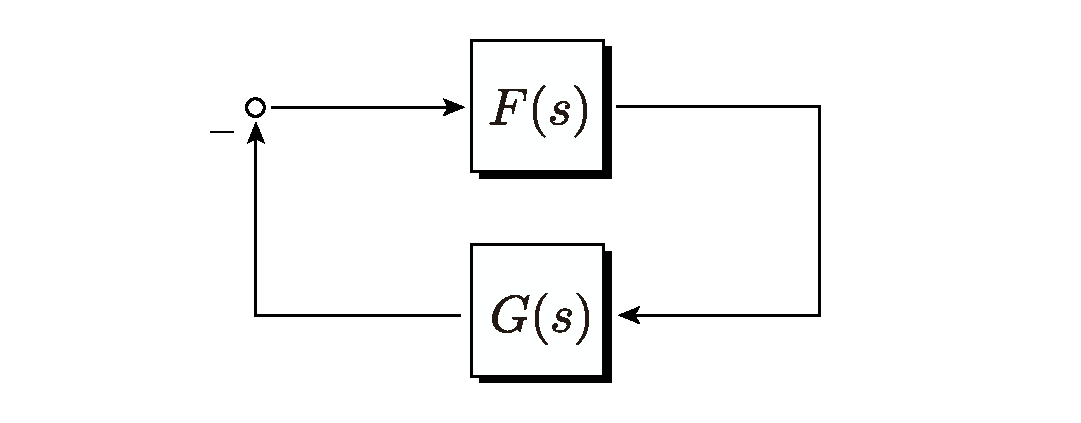
\includegraphics[width = .99\linewidth]{figs/staFG}
    \subcaption{ }
  \end{minipage}
  \begin{minipage}{0.49\linewidth}
    \centering
    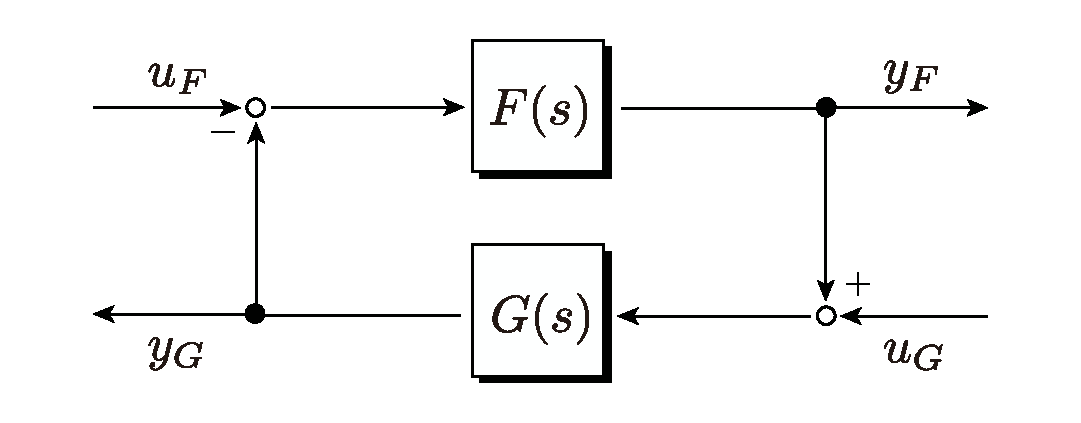
\includegraphics[width = .99\linewidth]{figs/staFGIO}
    \subcaption{ }
  \end{minipage}
  \caption{ネガティブ・フィードバック系}
  \label{fig:staFG}
  }
\end{figure}


\begin{定義}[伝達関数の正実性]\label{def:trpf}
正方な伝達関数$Q(s)$に対して
\begin{align}\label{eq:defOm0}
\Omega_0 := \left\{
\omega_0 \in \mathbb{R}: 
\mbox{ 純虚数$\bm{j} \omega_0$が$Q(s)$の極である}
\right\}
\end{align}
を定義する。
つぎの3条件が満たされるとき,$Q(s)$は\emph{正実}であると呼ぶ。
\begin{itemize}
\item $Q(s)$のすべての極の実部は非正である。
\item すべての$\omega \in [0,\infty)\setminus \Omega_0$に対して,$Q(\bm{j} \omega) + Q^{\sf T}(-\bm{j} \omega)$が半正定である。
\item 純虚数の極が存在するとき,それらの重複度は1であり,かつ,留数に対して
\begin{align*}
\lim_{s \rightarrow \bm{j} \omega_0} (s-\bm{j} \omega_0) Q(s) = \lim_{s\rightarrow \bm{j} \omega_0} \{ (s-\bm{j} \omega_0) Q(s)\}^{\sf *}\succeq 0
,\qquad
\forall \omega_0 \in \Omega_0
\end{align*}
が成り立つ。
\end{itemize}
\end{定義}

定義\ref{def:trpf}において,特に重要なものは1つ目と2つ目の条件である。
1つ目の条件は伝達関数の安定性を表している。
ただし,極の実部が0である場合も許容されている。
2つ目の条件は,伝達関数を虚軸上で評価したときの複素対称な部分の正定性に関するものである。
特に,$Q(s)$がスカラーの場合,すなわち,入力と出力がどちらもスカラーである場合には,2つ目の条件はすべての$\omega \in [0,\infty)\setminus \Omega_0$に対して$Q(\bm{j}\omega)$の実部が非負であることを表している。
ただし,$Q(s)$が行列である場合には,一般に
\begin{align*}
Q(\bm{j} \omega) + Q^{\sf T}(-\bm{j} \omega) \neq 2 \real\left[ Q(\bm{j} \omega) \right]
\end{align*}
であることに注意されたい。
なお,実数係数をもつ$Q(s)$に対しては$Q^{\sf T}( -\bm{j} \omega)$は$\{Q(\bm{j} \omega)\}^*$に等しい。
3つ目の条件は,$Q(s)$が純虚数の極をもつ場合の例外的なものであるが,例えば,式\ref{eq:trGs}の$G(s)$のように原点に極をもつ伝達関数を解析するために必要となる。

\begin{例}[並列された安定な1次系の正実性]\label{ex:Fspr1}
式\ref{eq:trFs}の$F(s)$が正実であることを確認してみよう。
まず,$F(s)$のすべての極の実部は負であるため,1つ目の条件は満たされている。
また,純虚数の極は存在しないため,3つ目の条件を考慮する必要はない。
さいごに,2つ目の条件について
\begin{align*}
\sfdiag \left( 
\frac{\omega_0}{ \bm{j} \omega M_i + D_i}
\right)
+
\left\{
\sfdiag \left( 
\frac{\omega_0}{\bm{j} \omega M_i + D_i}
\right)
\right\}^*
=
\sfdiag \left( 
\frac{2 \omega_0 D_i}{\omega^2 M_i^2 + D_i^2}
\right)
\end{align*}
であることから,すべての$\omega\in [0,\infty)$に対してその半正定性が示される。
なお,$\Omega_0=\emptyset$である。
\end{例}

\subsubsection{正実性に基づくフィードバック系の安定性解析}

以下では,伝達関数の正実性が,\ref{fig:staFG}(a)のようなフィードバック系の安定性を示すために有用な性質であることを説明する。
ただし,その準備として,伝達関数で表現されたフィードバック系に対する安定性を新たに定義する必要がある。
その理由は,\ref{fig:staFG}(a)では,$F(s)$や$G(s)$の入出力信号はフィードバック結合に使われてしまっており,外部から印加する入力信号や観測する出力信号が存在しないためである。
このことは,\ref{fig:staFG}(a)のフィードバック系には,入力と出力の関係を表す「伝達関数」そのものが定義されないことを意味する。
したがって,伝達関数に基づくフィードバック系の安定性解析に,定義\ref{def:trsta}の安定性の定義をそのまま用いることはできない。
以下の議論では,フィードバック系に対してつぎの安定性の定義を用いる。


\begin{定義}[フィードバック系の内部安定性]\label{def:fbsta}
\ref{fig:staFG}(a)のネガティブ・フィードバック系に対して,\ref{fig:staFG}(b)に示されるように入力と出力を追加することを考える。
このとき,$(u_F,u_G)$から$(y_F,y_G)$までの伝達関数
%\begin{align}\label{eq:defTs}
%\spliteq{
%& \underbrace{
%\mat{
%T_{y_Fu_F}(s)& T_{y_Fu_G}(s)\\
%T_{y_Gu_F}(s)& T_{y_G u_G}(s)
%}
%}_{T(s)}
%:= 
%\\
%& \mat{
%\bigl( I+ F(s)G(s) \bigr)^{-1}F(s) & -\bigl( I+ F(s)G(s) \bigr)^{-1}F(s) G(s) \\
%\bigl( I+ G(s)F(s) \bigr)^{-1}G(s)F(s) & \bigl( I+ G(s)F(s) \bigr)^{-1} G(s)
%}
%}
%\end{align}
\begin{align}\label{eq:defTs}
T(s)
:=\mat{
\bigl( I+ F(s)G(s) \bigr)^{-1}F(s) & -\bigl( I+ F(s)G(s) \bigr)^{-1}F(s) G(s) \\
\bigl( I+ G(s)F(s) \bigr)^{-1}G(s)F(s) & \bigl( I+ G(s)F(s) \bigr)^{-1} G(s)
}
\end{align}
に対して,$T(s)$を構成する4つの伝達関数がすべて安定であるとき,\ref{fig:staFG}(a)のネガティブ・フィードバック系は\emph{内部安定}であると呼ぶ。
\end{定義}

定義\ref{def:fbsta}における4つの伝達関数の安定性は,\ref{fig:staFG}(a)のフィードバック系を時間領域の微分方程式で表現した場合に,そのシステムが漸近安定となることと等価であることが知られている。
したがって,定義\ref{def:fbsta}は一見すると煩雑であるが,素朴に直感する時間領域における安定性と同義であると解釈すれば良い。
なお,式\ref{eq:trFs}の$F(s)$の定義から,\ref{fig:staFG}(b)における$u_F$と$y_F$の信号は,\ref{fig:blocklin}における$P_{\rm mech}^{\rm lin}$と$\omega_0 \Delta \omega^{\rm lin}$にそれぞれ対応することがわかる。
また,$y_G$は\ref{fig:blocklin}の$P^{\rm lin}$に対応する。
一方で,$u_G$は式\ref{eq:lindyn}の微分方程式には存在せず,伝達関数に基づくフィードバック系の内部安定性を定義するために現れた「仮想的な」入力であることに注意されたい。


\begin{figure}[t]
  \centering
  {
  \begin{minipage}{0.49\linewidth}
    \centering
    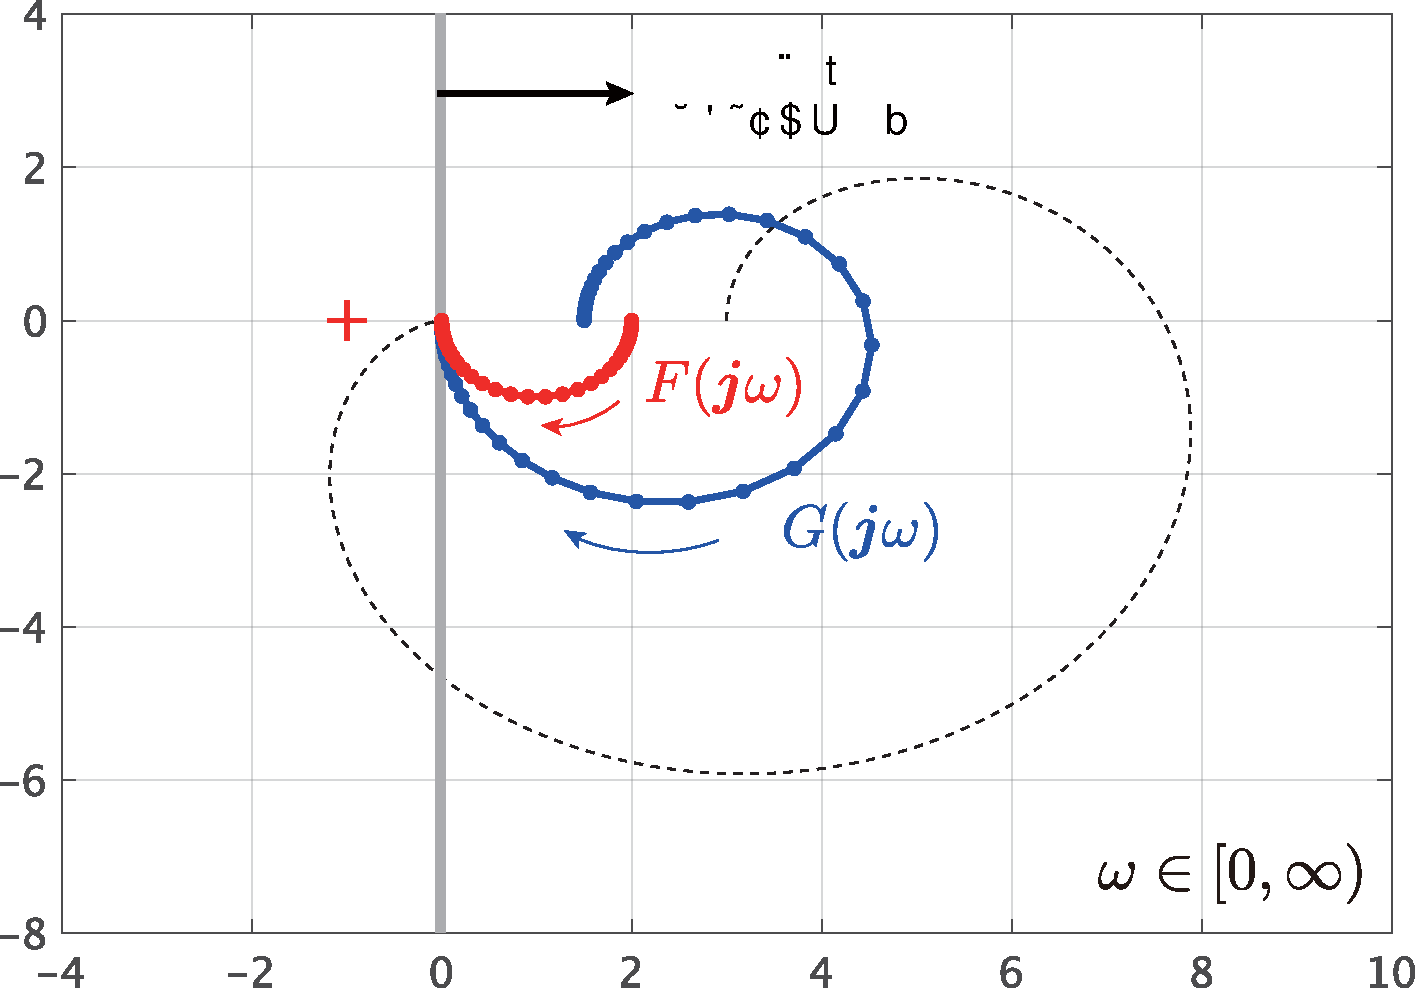
\includegraphics[width = .90\linewidth]{figs/nyquistFG}
    \subcaption{ $F(s)$と$G(s)$のナイキスト線図 }
  \end{minipage}
  \begin{minipage}{0.49\linewidth}
    \centering
    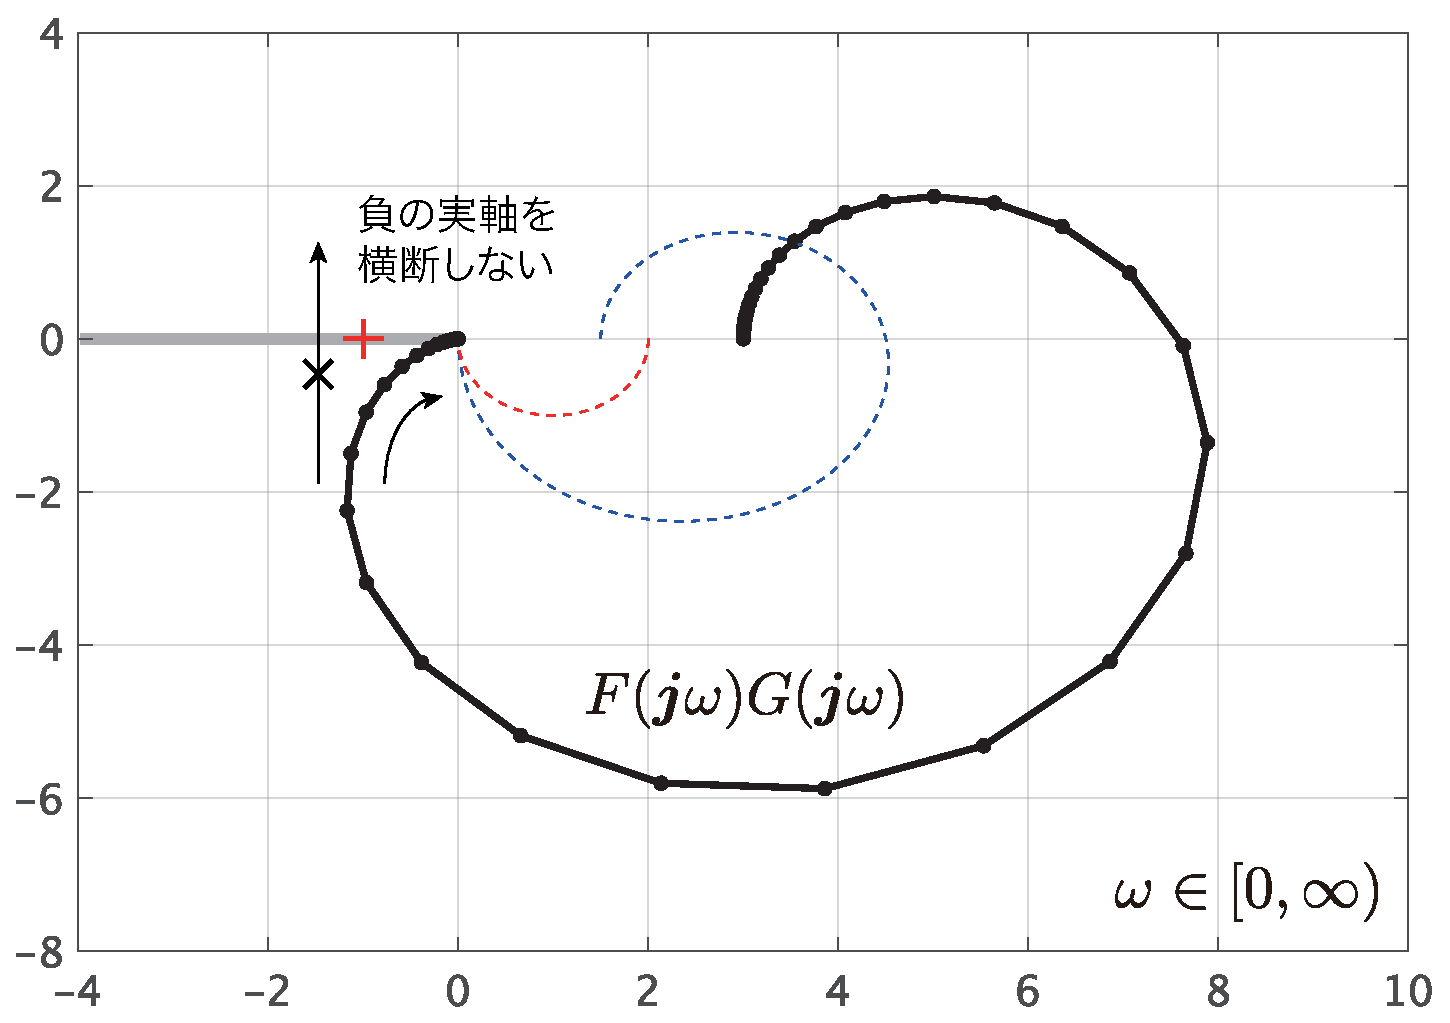
\includegraphics[width = .90\linewidth]{figs/nyquistFGop}
    \subcaption{  積$F(s)G(s)$のナイキスト線図 }
  \end{minipage}
  \caption{正実な伝達関数とそれらの積のナイキスト線図(赤十字は$-1 + 0 \bm{j}$の点を表す)}
  \label{fig:nyquistpr}
  }
\end{figure}


\begin{例}[正実な伝達関数のフィードバック系の安定性解析]
\label{ex:nyquistpr}
正実な伝達関数から構成されるネガティブ・フィードバック系の内部安定性をナイキストの安定判別法\red{(付録??)}の観点で考察してみよう。
説明の簡単化のため,\ref{fig:staFG}(a)における$F(s)$と$G(s)$はスカラーの伝達関数であるとする。
具体的には
\begin{align*}
F(s)=\frac{2}{s+1}
,\qquad
G(s)=\frac{3(12s+1)}{2(3s+1)(s+1)}
\end{align*}
と設定する。
このとき,$F(s)$と$G(s)$が正実な伝達関数であることは,\ref{fig:nyquistpr}(a)に示されるように,それらのナイキスト線図が複素平面上の虚軸より右側に存在することを意味している。
すなわち,$F(s)$と$G(s)$の周波数応答関数を
\begin{align*}
F(\bm{j} \omega) = |F(\bm{j} \omega)| e^{\bm{j} \angle F(\bm{j} \omega)}
,\qquad
G(\bm{j} \omega) = |G(\bm{j} \omega)| e^{\bm{j} \angle G(\bm{j} \omega)}
\end{align*}
と極座標で表示したときに,それらの位相$\angle F(\bm{j} \omega)$と$\angle G(\bm{j} \omega)$はどちらも,すべての$\omega$に対して$\left[ -\frac{\pi}{2},\frac{\pi}{2} \right]$の範囲に収まっていることを表している。
したがって,それらの積の周波数応答関数
\begin{align*}
F(\bm{j} \omega) G(\bm{j} \omega)
=
|F(\bm{j} \omega)| |G(\bm{j} \omega)| e^{\bm{j} \left\{\angle F(\bm{j} \omega) + \angle G(\bm{j} \omega)\right\}}
\end{align*}
の位相は,すべての$\omega$に対して$[-\pi,\pi]$の範囲にあることが導かれる。
この「位相が$[-\pi,\pi]$の範囲にある」という事実は,一見すると複素平面上のすべての位相を表しており特別な意味がないように見えるが,重要な点は「積の周波数応答関数のナイキスト線図は,負の実軸を横断するような軌跡は描かないこと」を表していることである。
この様子を\ref{fig:nyquistpr}(b)に示している。
したがって,$F(s)$と$G(s)$の積のナイキスト線図が,それらのネガティブ・フィードバック系の内部安定性を特徴づける$-1 + 0 \bm{j}$の点を右に見ながら周回しないことが結論づけられる。

しかしながら,$F(s)$と$G(s)$の正実性だけでは,積のナイキスト線図が$-1 + 0 \bm{j}$の点の上を「ちょうど通過する」ような安定限界となる場合が含まれている。
実応用においては,このような状況,すなわち
\begin{align*}
F(\bm{j} \omega_0) G(\bm{j} \omega_0) = -1 + 0 \bm{j}
\end{align*}
となる$\omega_0$が存在するような状況は,$F(s)$と$G(s)$を意図的に選ばない限りはほとんど起こらないが,数学的に厳密にフィードバック系の内部安定性を示すためには,正実性よりも少しだけ強い条件を$F(s)$や$G(s)$に課す必要がある。
この「少しだけ強い条件」の与え方には様々なものが考えられる。
例えば,すべての$\omega \in [0,\infty)$に対して,$F(\bm{j} \omega)$の位相が$ \left[-\frac{\pi}{2},\frac{\pi}{2} \right]$の境界には触れないこと,すなわち,$\left(-\frac{\pi}{2},\frac{\pi}{2} \right)$の範囲にあることがわかるだけで,$F(s)$と$G(s)$のネガティブ・フィードバック系の内部安定性が数学的に証明できる。
\end{例}


例\ref{ex:nyquistpr}で示されているように,伝達関数の正実性はフィードバック系の内部安定性を議論するために有用である。
しかしながら,注目する伝達関数が式\ref{eq:trFs}の$F(s)$のように単純なものではない場合には,その伝達関数が正実かどうかを解析的に判断することは難しい。

一方で,式\ref{eq:lindyn}のような微分方程式を解析する場合には,ラプラス領域の伝達関数に対して,「時間領域での状態空間実現をあらかじめ知っている」ことに注意されたい。
つぎの事実は,システム制御理論において\emph{正実補題}(positive real lemma)として知られているものであり\cite{rantzer1996kalman},時間領域での状態空間実現に基づいて伝達関数の正実性を判定することを可能にする。

\begin{補題}[正実補題]\label{lem:prlem}
安定かつ正方な伝達関数$Q(s)$に対して,その時間領域における実現のひとつが
\begin{align}\label{eq:realQs}
Q: \simode{
\dot{x}_Q &= A x_Q + B u_Q\\
y_Q &= C x_Q + D u_Q
}
\end{align}
で与えられているとする。
このとき,ある対称かつ正定な行列$P$が存在して
\begin{align}\label{eq:prlem}
\mat{
A^{\sf T}P+PA & PB-C^{\sf T} \\
B^{\sf T} P -C & -(D+D^{\sf T})
}\preceq 0
\end{align}
が満たされるならば,$Q(s)$は正実である。
特に,式\ref{eq:realQs}において\red{$(A,B)$が可制御}であるならば,式\ref{eq:prlem}の正定解$P$が存在することと$Q(s)$が正実であることは等価である。
\end{補題}

\begin{証明}
後半の等価性の証明には,本書で扱わない概念が必要となるため,ここでは前半の十分性の証明のみを示す。
式\ref{eq:prlem}より,任意の複素ベクトル$\bm{x}$と$\bm{u}$に対して
\begin{align}\label{eq:quadxu}
\mat{\bm{x} \\ \bm{u}}^*
\Biggl(
\mat{
0 & -C^{\sf T}\\
-C & - (D+D^{\sf T})
}
+
\mat{
A^{\sf T}P+PA & PB \\
B^{\sf T} P  & 0
}
\Biggr)
\mat{\bm{x}\\\bm{u}} \leq 0
\end{align}
が成り立つ。
ここで,一般に$\sftrace(XY)=\sftrace(YX)$であることを用いると
\begin{align*}
\mat{\bm{x}\\ \bm{u}}^*
\mat{
A^{\sf T}P+PA & PB \\
B^{\sf T} P  & 0
}
\mat{\bm{x}\\\bm{u}}
 =
\sftrace\left(
P\left\{
\bm{x}(A\bm{x}+B\bm{u})^* + (A\bm{x}+B\bm{u})\bm{x}^*
\right\}
\right)
\end{align*}
が得られる。
さらに,\red{付録の補題??}を用いることにより,$\bm{x}\neq 0$かつ
\begin{align}\label{eq:xstar}
\bm{x}(A\bm{x}+B\bm{u})^* + (A\bm{x}+B\bm{u})\bm{x}^*=0
\end{align}
であることと,ある$\omega \in \mathbb{R}\cup\{\infty\}$に対して
$A\bm{x}+B\bm{u}=\bm{j}\omega \bm{x}$が成り立つことが等価であることがわかる。
したがって,式\ref{eq:xstar}が成り立つすべての$\bm{x}\neq 0$と$\bm{u}$の組,すなわち,任意の$\bm{u}$と$\omega$により構成される非零の$\bm{x}=(\bm{j}\omega I -A)^{-1}B \bm{u}$に対して式\ref{eq:quadxu}の不等式を考えることにより,
\begin{align*}
\mat{(\bm{j}\omega I -A)^{-1}B \bm{u} \\\bm{u}} ^*
\mat{
0 & -C^{\sf T}\\
-C & - (D+D^{\sf T})
}
\mat{(\bm{j}\omega I -A)^{-1}B \bm{u} \\\bm{u}} 
\leq 0
\end{align*}
が,$B\bm{u}\neq 0$を満たす任意の$\bm{u}$と$\omega$に対して成り立つことがわかる。
なお,$D+D^{\sf T}$は半正定であることから,この不等式は$B\bm{u}= 0$であるような$\bm{u}$に対しても成り立つ。
したがって,式\ref{eq:prlem}が成り立つ正定な$P$が存在するのであれば,任意の$\bm{u}$と$\omega$に対して
\begin{align*}
\bm{u}^*
\left[
C(\bm{j}\omega I -A)^{-1}B + D
+
\left\{
C(\bm{j}\omega I -A)^{-1}B + D
\right\}^*
\right]
\bm{u} \geq 0
\end{align*}
が成り立つことが導かれる。
これは$Q(s)$が正実であることを意味する。
\end{証明}

正定行列$P$が式\ref{eq:prlem}の行列不等式を満たすことは,ある行列$L$と$W$が存在して
\begin{align}\label{eq:prlemeq}
\spliteq{
A^{\sf T}P+PA + L^{\sf T}L &= 0
,\qquad
W^{\sf T}W = D + D^{\sf T} \\
PB + L^{\sf T}W &= C^{\sf T}
}
\end{align}
が成り立つことと等価であることも知られている。
一般に,$P$を数値的に探索する場合には式\ref{eq:prlem}の不等式表現が都合が良いことが多い。
一方で,数学的な解析を行う場合には式\ref{eq:prlemeq}の方程式表現が都合が良い場合もあるため,目的に応じて2つの等価表現が使い分けられている。


\begin{例}[並列された安定な1次系に対する正実補題]\label{ex:Fspr2}
補題\ref{lem:prlem}を用いて式\ref{eq:trFs}の$F(s)$の正実性を確認してみよう。
式\ref{eq:Fss}は$F(s)$の時間領域における実現であることから,補題\ref{lem:prlem}の行列に当てはめて考えると
\begin{align*}
A = -\sfdiag \left( 
\frac{D_i}{ M_i} 
\right)
,\qquad 
B= \sfdiag \left( 
\frac{1}{ M_i} 
\right)
,\qquad
C= \omega_0 I 
,\qquad
D=0
\end{align*}
となる。
このとき,$P=\omega_0 \sfdiag(M_i)$と選べば,式\ref{eq:prlem}の行列不等式に対して
\begin{align*}
\mat{
-2 \sfdiag \left( 
\omega_0 D_i
\right)
 & 0 \\
0 & 0
}\preceq 0
\end{align*}
が得られるため,$F(s)$が正実であることが結論づけられる。
なお,この例のように,出力に入力が直接的に現れないシステム,すなわち,$D=0$であるシステムについては,その伝達関数の正実性は
\begin{align}\label{eq:Dzero}
A^{\sf T}P+PA \preceq 0
,\qquad 
PB=C^{\sf T}
\end{align}
を満たす正定な$P$が存在することと等価である。
ただし,$(A,B)$は可制御とする。


式\ref{eq:trFs}に対する座標変換として,$\tilde{x}_f := \omega_0 x_f$を考えてみよう。
このとき,$F(s)$の別の実現として
\begin{align*}
F: \simode{
\dot{\tilde{x}}_f &= \textstyle - \sfdiag \left( 
\frac{D_i}{ M_i} 
\right)
\tilde{x}_f
+ 
\omega_0 \sfdiag \left( 
\frac{1}{ M_i} 
\right)
 u_f \\
y_f &=  \tilde{x}_f
}
\end{align*}
が得られる。
この実現に対しては,$P=\omega_0^{-1} \sfdiag(M_i)$が式\ref{eq:prlem}の行列不等式の解として得られることがわかる。
このように,式\ref{eq:prlem}の行列不等式の解は,その状態空間実現に依存して変化することに注意されたい。
\end{例}

式\ref{eq:Fss}の$F$のように,入力が出力に直接的に現れないシステムの場合,すなわち,出力が状態変数の線形結合のみで記述される場合,その伝達関数の分母多項式の次数は分子多項式の次数よりも厳密に大きい。
このような伝達関数は,\emph{厳密にプロパー}な伝達関数と呼ばれる。
\ref{fig:staFG}(a)において,$F(s)$と$G(s)$の両方が厳密にプロパーでない場合には,それらのフィードバック系が定義されない場合があることに注意されたい。
これは,$F(s)$への入力信号が瞬時的にその出力信号として現れ,その出力信号が$G(s)$を通して瞬時的に$F(s)$にフィードバックされるような,入出力信号の瞬時的な無限ループが生じ得るためである。
なお,$F(s)$と$G(s)$の少なくともどちらか一方が厳密にプロパーであればそのような問題は生じないため,以下では必要に応じて伝達関数が厳密にプロパーであることを条件として課す。

つぎの補題が示すように,2つの正実な伝達関数によるネガティブ・フィードバック系は正実性をもつ。


\begin{補題}[正実な伝達関数のフィードバック系]\label{lem:prpre}
\ref{fig:staFG}(b)において,伝達関数$F(s)$と$G(s)$はどちらも正実であるとする。
ただし,$F(s)$と$G(s)$の少なくともどちらか一方は厳密にプロパーであるとする。
このとき,式\ref{eq:defTs}の$T(s)$によって定義される$(u_F,u_G)$から$(y_F,y_G)$までの伝達関数は正実である。
\end{補題}

\begin{証明}
時間領域において,$F(s)$と$G(s)$のネガティブ・フィードバック系は
\begin{align*}
F: \simode{
\dot{x}_F &= A_F x_F + B_F u_F\\
y_F &= C_F x_F + D_F u_F ,
}
\qquad
G: \simode{
\dot{x}_G &= A_G x_G + B_G y_F\\
u_F &= -C_G x_G 
}
\end{align*}
と表せる。
ただし,$G(s)$が厳密にプロパーである場合を考えているが,$F(s)$が厳密にプロパーである場合も同様である。
このとき,フィードバック系の状態方程式をひとつにまとめると
\begin{align*}
\mat{
\dot{x}_F \\ \dot{x}_G
}
 =
 \underbrace{
\mat{
A_F & -B_F C_G\\
B_G C_F & A_G - B_G D_F C_G
}
}_{A_T}
\mat{x_F \\ x_G}
+
\underbrace{
\mat{
B_F & 0\\
B_G D_F & B_G
}
}_{B_T}
\mat{u_F \\ u_G}
\end{align*}
が得られる。
同様に,出力方程式は
\begin{align*}
\mat{
y_F \\ y_G
}
 =
\underbrace{
\mat{
C_F & -D_F C_G\\
0 & C_G
}
}_{C_T}
\mat{x_F \\ x_G}
+ 
\underbrace{
\mat{
D_F & 0\\
0 & 0
}
}_{D_T}
\mat{u_F \\ u_G}
\end{align*}
とまとめられる。
定義より,$T(s) = C_T (sI -A_T)^{-1}B_T + D_T$である。
ここで,$F(s)$と$G(s)$の正実性の仮定から
\begin{align}\label{eq:asumpr}
\mat{
A_F^{\sf T}P_F+P_F A_F & P_FB_F-C_F^{\sf T} \\
B_F^{\sf T} P_F -C_F & -(D_F+D_F^{\sf T})
}\preceq 0
,\qquad
\simode{
&A_G^{\sf T}P_G+P_GA_G \preceq 0\\
&P_GB_G=C_G^{\sf T}
}
\end{align}
を満たす正定な$P_F$と$P_G$が存在する。
また,$P_F$と$P_G$をブロック対角に並べた行列を$P_T$とすると
\begin{align*}
A_T^{\sf T}P_T+P_T A_T 
&=
\mat{
A_F^{\sf T}P_F+P_F A_F & (C_F^{\sf T} -P_F B_F) C_G \\
C_G^{\sf T} (C_F^{\sf T} -P_F B_F)^{\sf T} & 
A_G^{\sf T}P_G+P_GA_G - C^{\sf T}_G (D_F + D_F^{\sf T})C_G
},
\\
P_T B_T &= \mat{
P_F B_F & 0 \\
C_G^{\sf T} D_F & C_G^{\sf T}
}
\end{align*}
が得られる。
ただし,式\ref{eq:asumpr}右の等式を用いた。
したがって
\begin{align}\label{eq:augpr}
\mat{
A_T^{\sf T}P_T+P_T A_T & P_T B_T - C_T^{\sf T} \\
B_T^{\sf T} P_T -C_T & -(D_T+D_T^{\sf T})
}
=
\mat{
X + Y & 0\\
0 & 0
}
\end{align}
となる。
ただし
\begin{align*}
X&:= 
\mat{
A_F^{\sf T}P_F+P_F A_F & -(P_FB_F-C_F^{\sf T})C_G & P_FB_F-C_F^{\sf T} \\
-C_G^{\sf T}(P_FB_F-C_F^{\sf T})^{\sf T} & - C^{\sf T}_G (D_F + D_F^{\sf T})C_G & C^{\sf T}_G (D_F + D_F^{\sf T})\\
(P_FB_F-C_F^{\sf T})^{\sf T} & (D_F + D_F^{\sf T})C_G & -(D_F + D_F^{\sf T})
},
\\
Y &:= 
\mat{
0&0&0\\
0&A_G^{\sf T}P_G+P_GA_G&0\\
0&0&0
}
\end{align*}
である。
式\ref{eq:asumpr}右の不等式より,$Y$は半負定であることから,式\ref{eq:augpr}の半不定性を示すためには,$X$が半不定であることを示せば良い。
実際,$X$は
\begin{align*}
X=
\mat{
I & 0 \\
0 & -C_G^{\sf T} \\
0 & I
}
\mat{
A_F^{\sf T}P_F+P_F A_F & P_FB_F-C_F^{\sf T} \\
B_F^{\sf T} P_F -C_F & -(D_F+D_F^{\sf T})
}
\mat{
I & 0 \\
0 & -C_G^{\sf T} \\
0 & I
}^{\sf T}
\end{align*}
と書き換えられることから,式\ref{eq:asumpr}左の不等式によって,式\ref{eq:augpr}の半不定性が示される。
これは$F(s)$と$G(s)$のフィードバック系が正実であることを意味している。
\end{証明}

補題\ref{lem:prpre}に示されている正実性が保存される性質は,式\ref{eq:lindyn}の近似線形モデルを伝達関数に基づき解析する場合にも有用である。
例\ref{ex:Fspr1}や例\ref{ex:Fspr2}で示されているように,式\ref{eq:trFs}の$F(s)$は正実である。
このとき,式\ref{eq:trGs}の$G(s)$の正実性が示されるのであれば,それらのネガティブ・フィードバック系は正実となることから,少なくとも式\ref{eq:lindyn}の内部状態は発散しないことが保証できる。
一方で,$F(s)$と$G(s)$が正実であることだけでは,フィードバック系の内部安定性を数学的に保証することはできない。
この内部安定性を示すために,つぎの事実が利用できる。

\begin{補題}[正定行列フィードバックによる正実な伝達関数の安定化]\label{lem:posfb}
\ref{fig:staFG}(a)において,伝達関数$F(s)$は正実かつ厳密にプロパーであり,$G(s)$は対称行列$G_0$であるとする。
このとき,$G_0$が正定であるならば,そのネガティブ・フィードバック系は内部安定である。
\end{補題}

\begin{証明}
\red{ナイキストで言ったほうが早いかも?}
時間領域において,$F(s)$と$G(s)$のネガティブ・フィードバック系は
\begin{align*}
F: \simode{
\dot{x}_F &= A x_F + B u_F\\
y_F &= C x_F ,
}
\qquad
G: u_F = - G_0 y_F
\end{align*}
と表せる。
ただし,$F$は最小実現であるものとする。
この表現から,$u_F$と$y_F$を代入により消去すると,フィードバック系の簡潔な表現として
\begin{align*}
\dot{x}_F = (A -B G_0 C) x_F
\end{align*}
が得られる。
正実補題から,式\ref{eq:Dzero}を満たすある正定な$P$が存在することに注意して,
\red{リアプノフ関数}の候補として$V(x_F):= x_F^{\sf T} P x_F$と選ぶと
\begin{align*}
\spliteq{
\frac{d}{dt} V(x_F) &= \dot{x}_F^{\sf T} P x_F + x_F^{\sf T} P \dot{x}_F\\
&= x_F^{\sf T} (\underbrace{A^{\sf T}P +PA - 2 C^{\sf T}G_0 C}_{M})x_F 
}
\end{align*}
が得られる。
\red{ここで,$(C,A)$は可観測であることから$M$は負定である。}
\end{証明}





\begin{例}[正実性に基づくフィードバック系の安定性解析]\label{ex:entsys}
補題\ref{lem:prpre}と補題\ref{lem:posfb}を組み合わせることにより,\ref{fig:staFG}(a)のフィードバック系の内部安定性を解析してみよう。
ただし,以下では,式\ref{eq:trGs}の$G(s)$が正実であることを仮定して議論する。
まず,式\ref{eq:Fss}の$F(s)$の状態空間実現について,それ自身が正実な伝達関数と正定な行列のネガティブ・フィードバック系であるとみなす。
具体的には,$F$を2つに分解することにより
\begin{align*}
F_0 &:\simode{
\dot{x}_f &= \textstyle - \sfdiag \left( 
\frac{D_i}{ M_i} - \kappa_i 
\right)
x_f
+ \sfdiag \left( 
\frac{1}{ M_i} 
\right)
(u_f + v_f) \\
y_f &= \omega_0 x_f,
}
\\
K&: y_k = \sfdiag \left( \frac{ M_i \kappa_i}{\omega_0} \right) y_f
,\qquad
v_f = - y_k
\end{align*}
とする。
仮想的な入出力である$v_f$と$y_k$を代入により消去すれば,この$F_0$と$K$のフィードバック系が式\ref{eq:Fss}に一致することは容易にわかる。
この分解は\ref{fig:Fdec}において点線のブロックで示されている。
また,$\kappa_i \in \left(0,\frac{D_i}{M_i} \right)$である適当な$\kappa_i$を選べば$F_0$は正実であり,$K$は正定行列による静的なフィードバックを表すことがわかる。
一方で,$G(s)$の正実性を仮定していることから,$F_0(s)$と$G(s)$を
\begin{align*}
F_0&:\simode{
\dot{x}_f &= \textstyle - \sfdiag \left( 
\frac{D_i}{ M_i} - \kappa_i 
\right)
x_f
+ \sfdiag \left( 
\frac{1}{ M_i} 
\right)
(u_f + v_f)
\\
y_f &= \omega_0 x_f,
}
\\
G&: \simode{
\dot{x}_g &= A_g x_g + B_g y_f\\
y_g &= C_g x_g, 
}
\qquad
u_f = -y_g
\end{align*}
のようにフィードバック結合した場合において,$v_f$から$y_f$までの伝達関数は正実となる。
したがって,\ref{fig:Fdec}のように,全体系は$F_0(s)$と$G(s)$から構成される正実な伝達関数に,$K$という正定行列のフィードバックを加えた系であるとみなすことができる。
これは\ref{fig:staFG}(a)のフィードバック系が内部安定であることを意味している。
\end{例}

\begin{figure}[t]
\centering
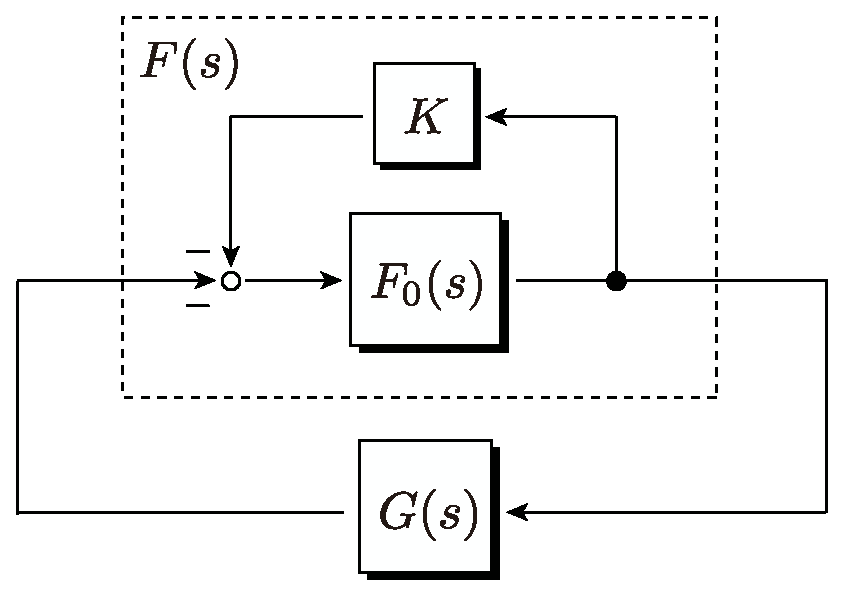
\includegraphics[width = .45\linewidth]{figs/Fdec}
\caption{正実性に基づくフィードバック系の内部安定性の保証}
\label{fig:Fdec}
\end{figure}

例\ref{ex:entsys}で示されているように,式\ref{eq:Fss}の$F(s)$が安定な1次系の並列であるという事実から,式\ref{eq:trGs}の$G(s)$が正実であれば\ref{fig:staFG}(a)のフィードバック系が内部安定であることが示される。
しかしながら,この内部安定性が,\ref{fig:blocklin}のフィードバック系の内部安定性を必ずしも意味しないことに注意されたい。
実際,式\ref{eq:eqset}が示すように,式\ref{eq:lindyn}の近似線形モデルには不変な固有空間が存在するため漸近安定ではない。
したがって,\ref{fig:blocklin}のフィードバック系は内部安定にはならない。
この相違は,\ref{fig:blocklin}を\ref{fig:staFG}(a)に変換して,積分器を含むいくつかのブロックを$G(s)$としてまとめたことにより,$G(s)$の内部で積分器の原点極が零点と相殺されていることに起因する。
次節では,この$G(s)$の内部の\red{極零相殺}にも注意して,より精密に近似線形モデルの同期を解析していく。

\subsection{正実性に基づく近似線形モデルの同期解析\advanced}\label{sec:syncanp}


\subsubsection{近似線形モデルの正実性}

式\ref{eq:sysmats}のシステム行列に現れた関数$k_{ij}(\delta_{ij}^{\star})$や$h_{ij}(\delta_{ij}^{\star})$には,式\ref{eq:defGam}で定義される$\bm{\mathit{\Gamma}}$の逆行列の実部や虚部が混在しており,解析的な扱いは容易ではない。
一方で,アドミタンス行列$\bm{Y}$の実部が0であるとき,$\bm{\mathit{\Gamma}}$は実対称かつ正定な行列となるため,式\ref{eq:sysmats}のシステム行列にも対称性や歪対称性などの扱いやすい構造が現れる。

一般に,アドミタンス行列の非対角要素の実部はすべて非負であることから,定理\ref{thm:PQ}より,アドミタンス行列の実部が0であることが,系統全体での有効電力の送電損失が0となるための必要十分条件であることがわかる。
これらの事実に基づき,つぎの定義を導入する。

\begin{定義}[無損失な送電網]\label{def:lless}
式\ref{eq:Ypig}のアドミタンス行列$\bm{Y}$の実部が0であるとき,送電網は\emph{無損失}であると呼ぶ。
\end{定義}

以下では,送電網が無損失であることが,式\ref{eq:trGs}の$G(s)$の正実性を特徴づけることを示す。
その準備として,正実性と対になる概念である伝達関数の負虚性(negative imaginaryness)を導入する\cite{petersen2010feedback,xiong2010negative}。

\begin{定義}[伝達関数の負虚性]
\label{def:trni}
原点に極をもたない正方な伝達関数$Q(s)$に対して,式\ref{eq:defOm0}の$\Omega_0$を定義する。
つぎの3条件が満たされるとき,$Q(s)$は\emph{負虚}であると呼ぶ。
\begin{itemize}
\item $Q(s)$のすべての極の実部は非正である。
\item すべての$\omega \in (0,\infty)\setminus \Omega_0$に対して,$\bm{j}\left\{Q(\bm{j} \omega) - Q^{\sf T}(-\bm{j} \omega) \right\}$が半正定である。
\item 純虚数の極が存在するとき,それらの重複度は1であり,かつ,留数に対して
\begin{align*}
\lim_{s \rightarrow \bm{j} \omega_0} (s-\bm{j} \omega_0) \bm{j} Q(s) = 
\lim_{s\rightarrow \bm{j} \omega_0} \{ (s-\bm{j} \omega_0) \bm{j} Q(s)\}^{\sf *}\succeq 0
,\quad
\forall \omega_0 \in \Omega_0
\end{align*}
が成り立つ。
\end{itemize}
\end{定義}

定義\ref{def:trpf}の正実性が,伝達関数の複素対称な部分に関する半正定性により定義されていたのに対して,定義\ref{def:trni}の負虚性は,伝達関数の複素歪対称な部分に関する半正定性により定義されている。
特に,$Q(s)$がスカラーの場合には,
\begin{align*}
\bm{j}\left\{Q(\bm{j} \omega) - Q^{\sf T}(-\bm{j} \omega) \right\}
= 2 \imag[Q(\bm{j} \omega)]
\end{align*}
であることから,2つ目の条件はすべての$\omega \in (0,\infty)\setminus \Omega_0$に対して$Q(\bm{j}\omega)$の虚部が非負であることを表している。
なお,定義\ref{def:trni}では,定義\ref{def:trpf}と対になるように,$Q(s)$が虚軸上に極をもつことを許容しているが,以下の議論では安定な伝達関数に対して負虚性を考えるため,2つ目の条件のみに注目すれば良い。
補題\ref{lem:prlem}の正実補題の対として,つぎの事実が\emph{負虚補題}(negative imaginary lemma)として知られている。

\begin{補題}[負虚補題]
\label{lem:nilem}
安定かつ正方な伝達関数$Q(s)$に対して,その時間領域における実現の1つが式\ref{eq:realQs}
で与えられているとする。
このとき,$D$が対称であり,かつ,ある対称かつ正定な行列$P$が存在して
\begin{align}\label{eq:nilem}
A^{\sf T}P+PA \preceq 0
,\qquad
-PA^{-1}B = C^{\sf T}
\end{align}
が満たされるならば,$Q(s)$は負虚である。
特に,式\ref{eq:realQs}において\red{$(A,B)$が可制御}であるならば,$D$が対称であり,かつ,式\ref{eq:nilem}の正定解$P$が存在することと$Q(s)$が負虚であることは等価である。
\end{補題}

\begin{証明}
まず,$D$の対称性が$Q(s)$が負虚であるための必要条件であることを示すために
\begin{align*}
\lim_{\omega \rightarrow \infty} 
\bm{j}\left\{Q(\bm{j} \omega) - Q^{\sf T}(-\bm{j} \omega) \right\}
= \bm{j} (D - D^{\sf T})
\end{align*}
を考える。
ここで,$D$が対称でないならば,$D - D^{\sf T}$は非零であり,その固有値はすべて純虚数の組となる。
したがって,$\bm{j} (D - D^{\sf T})$が半正定であることは,$D$が対称であることと等価である。
なお,$D$が対称であるとき,
\begin{align*}
Q(\bm{j} \omega) - Q^{\sf T}(-\bm{j} \omega) = 
C(\bm{j} \omega I -A)^{-1} - \left\{ C( -\bm{j} \omega I -A)^{-1} \right\}^{\sf T}
\end{align*}
において$D$は現れないことから,$D=0$である場合のみを考えても一般性は失われない。

補題\ref{lem:prlem}を用いて題意を示す。
まず,式\ref{eq:nilem}の正定解$P$が存在するならば,$Q(s)$は負虚であることを示す。
定義より,厳密にプロパーな$Q(s)$が負虚であるための必要十分条件は,
$sQ(s)$が正実となることである。
ここで,$sQ(s)$は,式\ref{eq:realQs}において,$u_{Q}$から
$
\dot{y}_Q = CA x_Q + CB u_Q
$
までの伝達関数であることから
\begin{align}\label{eq:sQs}
sQ(s) = CA (sI - A)^{-1}B + CB
\end{align}
となる。
なお,$Q(s)$が安定であれば$sQ(s)$も安定である。
したがって,式\ref{eq:prlem}と等価な式\ref{eq:prlemeq}より,ある正定行列$P$および行列$L$と$W$が存在して
\begin{align}\label{eq:nicLW}
\spliteq{
A^{\sf T}P+PA + L^{\sf T} L &=0,
\qquad
PB + L^{\sf T} W = (CA)^{\sf T}
\\
CB + (CB)^{\sf T} & = W^{\sf T} W
}
\end{align}
が成り立つのであれば,$sQ(s)$は正実である。

以下では,式\ref{eq:nicLW}の条件と式\ref{eq:nilem}の条件が等価であることを示す。
式\ref{eq:nicLW}の1つ目の等式は式\ref{eq:nilem}左の不等式を意味する。
つぎに,2つ目の等式から
\begin{align}\label{eq:nicB}
B  = P^{-1}  (A^{\sf T} C^{\sf T} - L^{\sf T} W)
\end{align}
であり,これを3つ目の等式に代入することで
\begin{align*}
CP^{-1}  (A^{\sf T} C^{\sf T} - L^{\sf T} W) + 
\left\{
P^{-1}  (A^{\sf T} C^{\sf T} - L^{\sf T} W)
\right\}^{\sf T}
= W^{\sf T} W
\end{align*}
が得られる。
これを等価変形していくと
\begin{align*}
\spliteq{
& CP^{-1}  A^{\sf T} C^{\sf T}  + 
\left\{
CP^{-1}  A^{\sf T} C^{\sf T}
\right\}^{\sf T} \\
&= W^{\sf T} W + CP^{-1}L^{\sf T} W +\left\{ CP^{-1}L^{\sf T} W \right\}^{\sf T} \\
& = (W+LP^{-1}C^{\sf T})^{\sf T} (W+LP^{-1}C^{\sf T}) - CP^{-1} 
L^{\sf T} L P^{-1} C^{\sf T} \\
& = (W+LP^{-1}C^{\sf T})^{\sf T} (W+LP^{-1}C^{\sf T}) + CP^{-1}  A^{\sf T} C^{\sf T}  + 
\left\{
CP^{-1}  A^{\sf T} C^{\sf T}
\right\}^{\sf T} 
}
\end{align*}
が得られる。
ただし,$L^{\sf T} L$の変形に式\ref{eq:nicLW}の1つ目の等式を用いた。
これより,$W+LP^{-1}C^{\sf T}=0$が得られる。
式\ref{eq:nicB}から$W$を消去し,$L^{\sf T} L$を再び書き換えることにより,式\ref{eq:nilem}右の等式が導かれる。
したがって,式\ref{eq:nicLW}の条件と式\ref{eq:nilem}の条件は等価である。

以上の事実から,式\ref{eq:nilem}の正定解$P$が存在するならば,$sQ(s)$は正実である。
これは,厳密にプロパーな$Q(s)$が負虚であることを意味する。
逆に,$Q(s)$が負虚であり,式\ref{eq:realQs}による実現において$(A,B)$が可制御であるならば,$sQ(s)$は正実であり,式\ref{eq:sQs}による実現において$(A,B)$が可制御であることが導かれる。
したがって,式\ref{eq:nilem}の正定解$P$の存在が示される。
\end{証明}

以上の正実性と負虚性の定義に基づいて,式\ref{eq:trGs}の$G(s)$に対してつぎの事実が示される。

\begin{定理}\label{thm:EdynNI}
式\ref{eq:trGs}の伝達関数$H(s)$は安定であると仮定する。
このとき,$H(s)$が負虚であることは,送電網が無損失であることと等価である。
また,式\ref{eq:trGs}の伝達関数$G(s)$が正実であることは,
送電網が無損失であり,かつ
\begin{align}\label{eq:pdsp}
L-CA^{-1}B = (L-CA^{-1}B)^{\sf T} \succeq 0
\end{align}
が成り立つことと等価である。
\end{定理}

\begin{証明}
まず,$H(s)$が負虚であるならば,送電網が無損失であることを示す。
このためには,その対偶として,送電網が無損失でないならば,$H(s)$が負虚ではないことを示せば良い。
ここで,式\ref{eq:Ypig}の$\bm{Y}$の実部が0でない場合には$L$は非対称であることがわかる。
一方で,$H(s)$が負虚であるための必要条件は$L$が対称となることである。
したがって,送電網が無損失でないならば,$H(s)$は負虚ではないことが示される。


つぎに,送電網が無損失であるならば,$H(s)$は負虚であることを示す。
補題\ref{lem:nilem}より,$H(s)$が負虚であることを示すためには,$L$が対称であり,かつ
\begin{align}\label{eq:cndQ}
\tilde{A}^{\sf T}Q + Q\tilde{A} \preceq 0
,\qquad
Q\tilde{A}^{-1}\tilde{B}=C^{\sf T}
\end{align}
を満たす正定な行列$Q$が存在することを示せば良い。
ただし,
\begin{align*}
\tilde{A}:= \sfdiag \left( \frac{ 1 }{\tau_{{\rm d}i}} \right)
A
,\qquad
\tilde{B}:= \sfdiag \left( \frac{ 1 }{\tau_{{\rm d}i}} \right)
B
\end{align*}
とする。
ここで,送電網が無損失であるならば,式\ref{eq:Ypig}の$\bm{Y}$の実部は0であるため,式\ref{eq:Yred}の$\bm{Y}^{\rm red}$の実部$G_{ij}^{\rm red}$も0であることから,
\begin{align*}
k_{ij}(\delta_{ij}^{\star}) =
k_{ji}(\delta_{ji}^{\star})
,\qquad
h_{ij}(\delta_{ij}^{\star}) = 
- h_{ji}(\delta_{ji}^{\star}),\qquad
h_{ii}(\delta_{ii}^{\star}) = 0
\end{align*}
が成り立つ。
このとき,$L$は対称である。
また,$H(s)$は安定であることから
\begin{align*}
\tilde{A} = 
\sfdiag \left( \frac{X_{{\rm d}i} -  X_{{\rm q}i}}{\tau_{{\rm d}i}} \right)
\tilde{A}'
\end{align*}
において,$X_{{\rm q}i} > X_{{\rm d}i}$であることから
\[
\tilde{A}':=
\mat{
k_{11}(\delta_{11}^{\star}) & k_{12}(\delta_{12}^{\star}) & \cdots & k_{1N}(\delta_{1N}^{\star})\\
k_{21}(\delta_{21}^{\star}) &  k_{22}(\delta_{22}^{\star}) & \cdots & k_{2N}(\delta_{2N}^{\star})\\
  \vdots & \vdots & \ddots & \vdots\\
k_{N1}(\delta_{N1}^{\star}) &  k_{N2}(\delta_{N2}^{\star}) & \cdots & k_{NN}(\delta_{NN}^{\star})
}
- \sfdiag \left(
\frac{X_{{\rm d}i}}{X_{{\rm q}i}(X_{{\rm d}i}-X_{{\rm q}i})}
\right)
\]
は負定である。
したがって,$Q=-\tilde{A}'$は式\ref{eq:cndQ}を満たす正定行列となることから,$H(s)$が負虚であることが示される。


つぎに,$G(s)$に関する等価性を示す。
いま,$H(s)$は安定であることを仮定していることから,$G(s)$の虚軸上の極は原点のみであり,その重複度は1である。
したがって,$G(s)$が
正実であるための必要十分条件は,
\begin{align}\label{eq:Gpr}
G(\bm{j}\omega) + G^{\sf T}(-\bm{j}\omega) \succeq 0
,\qquad \forall \omega \in \mathbb{R}\setminus\{0\}
\end{align}
が成り立つこと,かつ
\begin{align}\label{eq:cndG0}
\lim_{s\rightarrow 0} s G(s) = \lim_{s\rightarrow 0} \{ s G(s)\}^{\sf T}\succeq 0
\end{align}
が成り立つことである。
送電網が無損失であるとき,式\ref{eq:Gpr}が成り立つことは
\begin{align}\label{eq:NIineq}
G(\bm{j}\omega) + G^{\sf T}(-\bm{j}\omega)
=
\frac{\bm{j}}{\omega} \left\{
H(\bm{j}\omega) - H^{\sf T}(-\bm{j}\omega)
\right\}
,\qquad \forall \omega \in \mathbb{R}\setminus\{0\}
\end{align}
より,$H(s)$が負虚であることから示される。
また,
\begin{align*}
\lim_{s\rightarrow 0} s G(s) =
L - C\tilde{A}^{-1}\tilde{B} = L - C A^{-1} B
\end{align*}
であることから,式\ref{eq:cndG0}の半正定性は式\ref{eq:pdsp}の条件に等しい。
なお,送電網が無損失であるとき,$L$は対称であり,
\begin{align*}
C\tilde{A}^{-1}\tilde{B} = C Q^{-1} C^{\sf T}
\end{align*}
も対称であることから,式\ref{eq:cndG0}の対称性も示される。

逆に,送電網が無損失でない,または,式\ref{eq:pdsp}の条件が満たされないならば$G(s)$が正実でないことを示す。
後者については,式\ref{eq:pdsp}の条件が式\ref{eq:cndG0}の条件に等しいことから明らかである。
また,送電網が無損失でないとき,$H(s)$は負虚ではないことから,
\begin{align*}
\lambda_{\rm min}\left[
\bm{j}
\left\{
H(\bm{j}(\omega_0 + \alpha )) - H^{\sf T}(-\bm{j}(\omega_0 + \alpha ))
\right\}
\right] < 0
,\qquad
\forall \alpha \in (0,\epsilon] 
\end{align*}
となるある点$\omega_0\geq 0$および十分に小さな$\epsilon >0$が存在する。
ただし,$\lambda_{\rm min}$は最小固有値を表す。
したがって,0ではないすべての$\omega \in (\omega_0, \omega_0+\epsilon] $に対して
$G(\bm{j} \omega) + G^{\sf T}(-\bm{j} \omega) $は半正定ではない。
\end{証明}

定理\ref{thm:EdynNI}は,送電網が無損失であることが,式\ref{eq:trGs}の伝達関数$G(s)$が正実であることを特徴づける条件の1つであることを示している。
なお,もう1つの条件である式\ref{eq:pdsp}の意味はつぎのように説明できる。
式\ref{eq:lindyn}の近似線形モデルにおいて,内部電圧の状態方程式である
\begin{align*}
\sfdiag(\tau_{{\rm d}i})
 \dot{E}^{\rm lin} = 
A E^{\rm lin}(t) + B \delta^{\rm lin}(t) 
+ V^{\rm lin}_{\rm field}(t)
\end{align*}
に注目する。
この微分方程式において,すべての時定数$\tau_{{\rm d}i}$が0に漸近する極限を考える。
これは「内部電圧が定常状態に達するために必要な時間が,$\delta^{\rm lin}(t)$や$V^{\rm lin}_{\rm field}(t)$が変動する時間と比較して十分に短いような極限を考えること」に相当する。
例えば,$\delta^{\rm lin}(t)$と$V^{\rm lin}_{\rm field}(t)$の時間変化が非常に緩やかであり,定数$\delta^{\rm lin}_0$と$V^{\rm lin}_{{\rm field}0}$とみなせると仮定すると,$E^{\rm lin}(t)$は一定の時間が経過すれば
\begin{align*}
E^{\rm lin}_0 = -A^{-1} B \delta^{\rm lin}_0
-A^{-1} V^{\rm lin}_{{\rm field}0}
\end{align*}
という値に漸近する。
ただし,$A$は安定である必要がある。
したがって,$E^{\rm lin}(t)$が定常状態に達する時間が十分に短い,すなわち,すべての時定数$\tau_{{\rm d}i}$が十分に小さい場合には,$E^{\rm lin}(t)$と比較して緩やかに変化する$\delta^{\rm lin}(t)$や$V^{\rm lin}_{\rm field}(t)$に対しても
\begin{align}\label{eq:spa}
E^{\rm lin}(t) \simeq  -A^{-1} B\delta^{\rm lin}(t)
- A^{-1} V^{\rm lin}_{\rm field}(t)
\end{align}
という近似が成り立つ。
このような状態変数の時間スケールの違いを利用して,収束が速い微分方程式を代数方程式で近似する方法は,システム制御理論において\emph{特異摂動近似}(singular perturbation approximation)と呼ばれている。
\red{実際,内部電圧の動特性は,機械的なタービンの動特性に比較して時定数が小さいため,このような特異摂動近似を介して電力系統モデルの挙動を解析することは有意義である。}
式\ref{eq:spa}が等号として成り立つものとして$\Delta \omega^{\rm lin}(t)$の微分方程式に代入すれば
\begin{align}\label{eq:spamodel}
\spliteq{
\mat{
\dot{\hat{\delta}}^{\rm lin} \\
\sfdiag(M_i) \Delta \dot{\hat{\omega}}^{\rm lin} 
}
&=
\mat{
 0 & \omega_0 I \\
  -(L-CA^{-1}B) & -\sfdiag(D_i)  \\
 }
\mat{
\hat{\delta}^{\rm lin} \\
\Delta \hat{\omega}^{\rm lin}
}
\\
&+
\mat{
0 & 0 \\
I & CA^{-1}
}
\mat{
P_{{\rm mech}}^{\rm lin} \\
V_{{\rm field}}^{\rm lin}
}
}
\end{align}
が得られる。
ただし,近似的な動特性であることを表すため状態変数を
$\hat{\delta}^{\rm lin}$,
$\Delta \hat{\omega}^{\rm lin}$として区別した。
また,内部電圧の近似的な値は
\begin{align*}
\hat{E}^{\rm lin}:=  -A^{-1} B \hat{\delta}^{\rm lin}
- A^{-1} V^{\rm lin}_{\rm field}
\end{align*}
として与えられる。
式\ref{eq:spamodel}の特異摂動近似システムは,線形2次振動子の結合系となっており,式\ref{eq:pdsp}の条件は,ばね定数をまとめた行列の半正定性を保証するものであることがわかる。
また,式\ref{eq:spamodel}の平衡点集合は
\begin{align}\label{eq:Msp}
\mathcal{M}_{\rm sp} := \sfspan 
\left\{
\mat{ \mathds{1}\\0 }
\right\}
\end{align}
である。

\begin{例}[特異摂動近似システムの初期値応答]
例\ref{ex:linsyssim}で扱った3つの発電機で構成される近似線形モデルに対して,式\ref{eq:spamodel}の特異摂動近似システムの初期値応答を確認してみよう。
\ref{fig:gamsta}と同じ設定で,特異摂動近似システムの初期値応答を重ねてプロットしたものが\ref{fig:timeexsp}である。
この例では,内部電圧の時定数がすべての発電機で$\tau_{{\rm d}i}=0.01$という相対的に小さな値に設定されているため,近似線形モデルと特異摂動近似システムの状態の軌道の差はほとんど生じていないことがわかる。
また,内部状態が式\ref{eq:Msp}の平衡点集合$\mathcal{M}_{\rm sp}$の点に収束していることもわかる。
\end{例}

\begin{figure}[t]
  \centering
  {
  \begin{minipage}{0.32\linewidth}
    \centering
    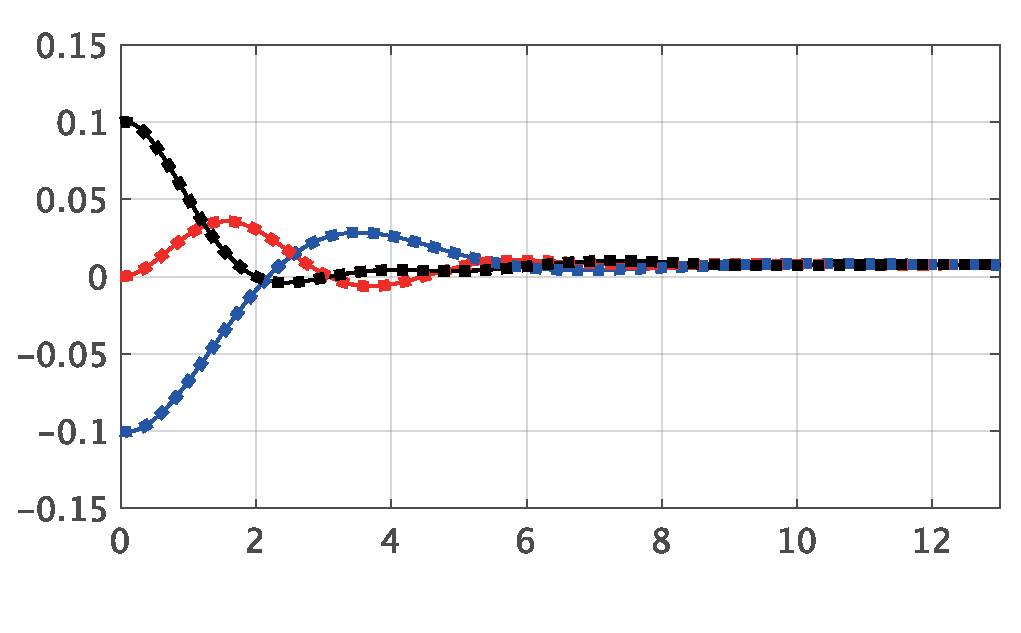
\includegraphics[width = .99\linewidth]{figs/deltasp}
    \subcaption{ 実線:$\delta^{\rm lin}$,点線:$\hat{\delta}^{\rm lin}$ }
  \end{minipage}
  \begin{minipage}{0.32\linewidth}
    \centering
    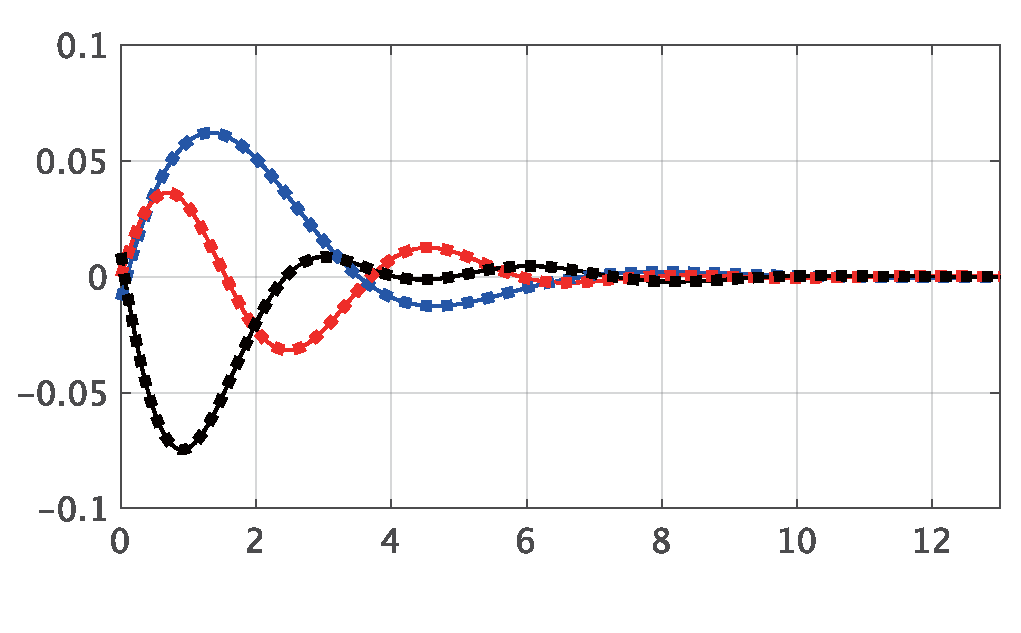
\includegraphics[width = .99\linewidth]{figs/omegasp}
    \subcaption{ 実線:$\Delta \omega^{\rm lin}$,点線:$\Delta \hat{\omega}^{\rm lin}$ }
  \end{minipage}
  \begin{minipage}{0.32\linewidth}
    \centering
    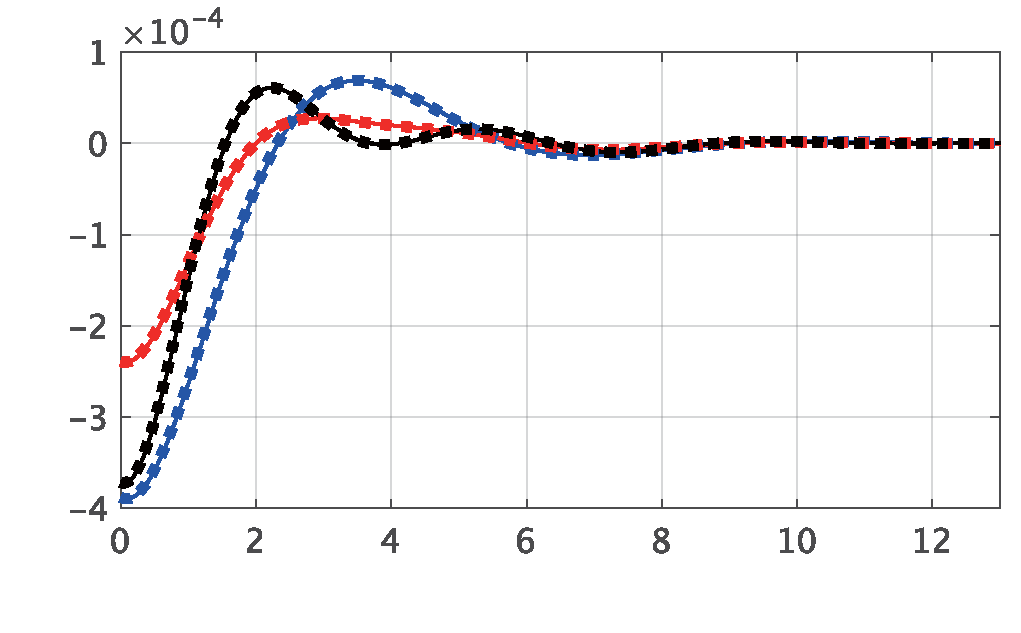
\includegraphics[width = .99\linewidth]{figs/Esp}
    \subcaption{ 実線:$E^{\rm lin}$,点線:$\hat{E}^{\rm lin}$}
  \end{minipage}
  \caption{近似線形モデルと特異摂動近似システムの初期値応答(青:発電機1,赤:発電機2,黒:発電機3)}
  \label{fig:timeexsp}
  }
\end{figure}

式\ref{eq:pdsp}の条件に基づいて,特異摂動近似システムの同期がつぎのように特徴づけられる。

\begin{定理}[特異摂動近似システムの同期]\label{thm:2ndsys}
式\ref{eq:spamodel}の特異摂動近似システムを考える。ただし,入力は恒等的に0とする。
任意の初期値および任意の正定数$M_i$,$D_i$に対して,内部状態が式\ref{eq:Msp}の平衡点集合$\mathcal{M}_{\rm sp}$のいずれかの点に収束するための必要条件は,式\ref{eq:nescon}および
\begin{align}\label{eq:eigreal}
\bm{\Lambda}(L-CA^{-1}B)\subseteq [0,\infty)
\end{align}
が成り立つことである。
ただし,$\bm{\Lambda}(\cdot)$は固有値の集合を表す。
特に,送電網が無損失であるとき,上記の収束性の必要十分条件は,式\ref{eq:nescon}および式\ref{eq:eigreal}が成り立つことである。
\end{定理}

\begin{証明}
まず,送電網が無損失である場合に,式\ref{eq:nescon}と式\ref{eq:eigreal}が成り立つことが,題意の収束性の十分条件であることを示す。
式\ref{eq:spamodel}の特異摂動近似システムは,式\ref{eq:trFs}の$F(s)$と
\begin{align*}
G_{\rm sp}(s):= \frac{1}{s} (L-CA^{-1}B)
\end{align*}
のネガティブ・フィードバック系として解釈できる。
送電網が無損失であるとき,$L-CA^{-1}B$は対称であるため,式\ref{eq:eigreal}の条件は式\ref{eq:pdsp}の条件,すなわち,$G_{\rm sp}(s)$が正実であることと等価である。
したがって,式\ref{eq:pdsp}が成り立つならば,例\ref{ex:entsys}の議論と同様にして,そのネガティブ・フィードバック系が内部安定であることが示される。
この内部安定性は,式\ref{eq:spamodel}から冗長な積分器を削除した
\begin{align*}
\spliteq{
\mat{
\dot{\hat{\delta}}^{\rm lin}_e \\
\sfdiag(M_i) \Delta \dot{\hat{\omega}}^{\rm lin} 
}
&=
\mat{
 0 & \omega_0 W \\
  -(L_0 -CA^{-1}B_0) & -\sfdiag(D_i)  \\
 }
\mat{
\hat{\delta}^{\rm lin}_e \\
\Delta \hat{\omega}^{\rm lin}
}
\\
&+
\mat{
0 & 0 \\
I & CA^{-1}
}
\mat{
P_{{\rm mech}}^{\rm lin} \\
V_{{\rm field}}^{\rm lin}
}
}
\end{align*}
が漸近安定であることと等価である。
したがって,任意の初期値および任意の正定数$M_i$,$D_i$に対して,システムの状態は$\mathcal{M}_{\rm sp}$のいずれかの点に収束することが示される。

つぎに,式\ref{eq:nescon}が必要であることは補題\ref{lem:nescon}の議論と同様に明らかであるため,式\ref{eq:eigreal}が成り立つことが題意の収束性の必要条件であることを示す。
このために,$K:=L-CA^{-1}B$として,つぎの2つの場合に分けて議論する。
\begin{itemize}
\item[(a)] $K$の固有値のうち,実部が負であるもの,または,純虚数であるのものが存在する。
\item[(b)] $K$の固有値のうち,実部が正であり,かつ,虚部が非零であるものが存在する。
\end{itemize}
まず,(a)である場合に,ある正定数$M_i$,$D_i$が存在して,式\ref{eq:spamodel}の特異摂動近似システムが不安定となることを示す。
以下では,すべての$i$に対して$M_i=1$,$D_i=d$と選ぶ。
また,正の定数倍に関してシステムの安定性は不変であるから,$\omega_0 =1$としても一般性は失われない。
このとき,式\ref{eq:spamodel}の固有方程式は
\begin{align*}
\mat{
0 & I \\
-K & -d I
}
\mat{v\\w}
=
\lambda \mat{v\\w}
\end{align*}
である。
この方程式から$w$を代入により消去すれば
\begin{align*}
\left(\lambda^2 I +d \lambda I + K
\right) v =0
\end{align*}
が得られる。
この固有方程式は,$v$が$K$の固有ベクトルであり,その固有値$\kappa$に対して
\begin{align*}
\lambda^2 + d\lambda +\kappa =0
\qquad
\Longleftrightarrow
\qquad
\lambda = \frac{-d \pm \sqrt{d^2-4\kappa} }{2}
\end{align*}
が成り立つことを意味する。
したがって,(a)である場合に,$\sqrt{d^2 - 4\kappa }$の実部が$d$より大きいことを示せば良い。
一般に,任意の複素数$\bm{z}$に対して
\begin{align*}
\real[\bm{z}] = \sqrt{ \real[\bm{z}^2 ] + (\imag[\bm{z}])^2 }
\end{align*}
と表せることから,$\bm{z} = \sqrt{d^2 - 4\kappa }$とすると
\begin{align*}
\real \Bigl[
\sqrt{d^2 - 4\kappa }
\Bigr]
=\sqrt{
d^2 - 4 \real[\kappa]
+
(\imag[ \bm{z} ])^2
}
\end{align*}
が得られる。
この値は,(a)である場合,すなわち,$\kappa$の実部が負,または,$\kappa$の実部が0かつ$\kappa$の虚部が非零である場合には,必ず$d$より大きい。
したがって,式\ref{eq:spamodel}の特異摂動近似システムは不安定である。

つぎに,(b)である場合を考える。
いま,$K$は実行列であるため,それが複素数の固有値をもつ場合には,虚部が負のものが必ず存在する。
その固有値を$\kappa$と表す。
このとき,$G_{\rm sp}(\bm{j} \omega)$は$\sigma (\bm{j} \omega):= \frac{\kappa}{\bm{j} \omega}$を固有値にもつ。
いま,ある適当な$\hat{\omega}\in (0,\infty)$に対して
\begin{align}\label{eq:Fspara}
-\real[\sigma(\bm{j} \hat{\omega})]  = \frac{D}{\omega_0}
,\qquad
-\imag[\sigma(\bm{j} \hat{\omega})]  = \frac{\hat{\omega} M}{\omega_0}
\end{align}
となるように定数$D$,$M$を選び,すべての$i$に対して$M_i=M$,$D_i=D$とすれば
\begin{align*}
F(\bm{j} \hat{\omega}) = - \frac{1}{ \sigma(\bm{j} \hat{\omega}) } I
\end{align*}
と表すことができる。
なお,$\kappa$の実部が正であり,虚部が負であることから,$D$と$M$は正である。
このとき,固有値$\sigma (\bm{j} \omega)$に対する$G_{\rm sp}(\bm{j} \hat{\omega})$の固有ベクトルを$v(\bm{j} \hat{\omega})$とすれば
\begin{align*}
\bigl\{ I+G_{\rm sp}(\bm{j} \hat{\omega})F(\bm{j} \hat{\omega})\bigr\}
v(\bm{j} \hat{\omega})
=0
\end{align*}
が得られる。
これは$\sfdet [I+G_{\rm sp}(\bm{j} \hat{\omega}) F(\bm{j} \hat{\omega})]=0$であることを意味する。
したがって,$F(s)$と$G_{\rm sp}(s)$のネガティブ・フィードバック系は内部安定ではない。
\end{証明}




定理\ref{thm:2ndsys}は,送電網が無損失であるとき,内部電圧の時定数が十分に小さい極限では,式\ref{eq:nescon}および式\ref{eq:eigreal}が成り立つことが,任意の慣性定数と制動係数に対して式\ref{eq:lindyn}の線形近似システムが同期を達成するための必要十分条件であることを意味している。
また,それら2つの条件は,送電網が無損失であるかどうかに関わらず,同期のための必要条件であることも示している。
特に,式\ref{eq:eigreal}の必要条件は,$L-CA^{-1}B$の固有値が非負の実数でない場合には,線形近似システムの同期が達成されないような発電機の定数が必ず存在することを示している。
本節の結論はつぎの定理にまとめられる。


\begin{定理}[線形近似システムの同期条件]\label{thm:sync}
式\ref{eq:lindyn}の線形近似システムを考える。
任意の初期値および任意の正定数$M_i$,$D_i$,$\tau_i$に対して,線形近似システムが同期するための必要条件は,
\begin{itemize}
\item[(i)] $A$が安定であること,かつ
\item[(ii)] 式\ref{eq:nescon}が成り立つこと,かつ
\item[(iii)] 式\ref{eq:eigreal}が成り立つこと
\end{itemize}
である。
特に,送電網が無損失であるとき,上記の収束性の必要十分条件は,条件(i)--(iii)が成り立つことである。
\end{定理}

\begin{証明}
送電網が無損失である場合に,条件(i)--(iii)が成り立つならば線形近似システムの同期が達成されることは,これまでの議論で示されている。
一方で,条件(ii)の必要性は補題\ref{lem:nescon}の議論で示されている。
また,条件(i)と条件(iii)は,定理\ref{thm:2ndsys}に示されているように,すべての$\tau_{{\rm d}i}$が十分に小さい極限において,偏差サブシステムが漸近安定となるための必要条件である。
\end{証明}

定理\ref{thm:sync}は,送電網が無損失である場合に,任意の発電機の定数に対して式\ref{eq:lindyn}の線形近似システムの同期が達成されるための必要十分条件を与えている。
また,送電網が無損失であるかどうかに関わらず,条件(i)--(iii)がその必要条件であることも示している。
なお,条件(i)は発電機の同期リアクタンスの値に部分的に依存しているが,条件(ii)や条件(iii)は,送電網のアドミタンス行列,内部電圧と発電機偏角差の定常値のみに関するものであり,発電機の物理定数には依存しないことに注意されたい。
また,$L-CA^{-1}B$は,\ref{fig:blocklin}において,内部電圧の時定数$\tau_{{\rm d}i}$が十分に小さい場合の発電機偏角$\delta^{\rm lin}$と有効電力$P^{\rm lin}$の入出力関係を表す行列,すなわち
\begin{align*}
\hat{P}^{\rm lin}(t) = (L-CA^{-1}B) \hat{\delta}^{\rm lin}(t)
- C A^{-1} V^{\rm lin}_{\rm field}(t)
\end{align*}
の第1項目に現れる行列である。
ただし,特異摂動近似を適用した場合の信号であることを表すため$\hat{P}^{\rm lin}$として区別した。
この定理を用いて,以下のように近似線形モデルの同期を解析することができる。


\begin{figure}[t]
  \centering
  {
  \begin{minipage}{0.32\linewidth}
    \centering
    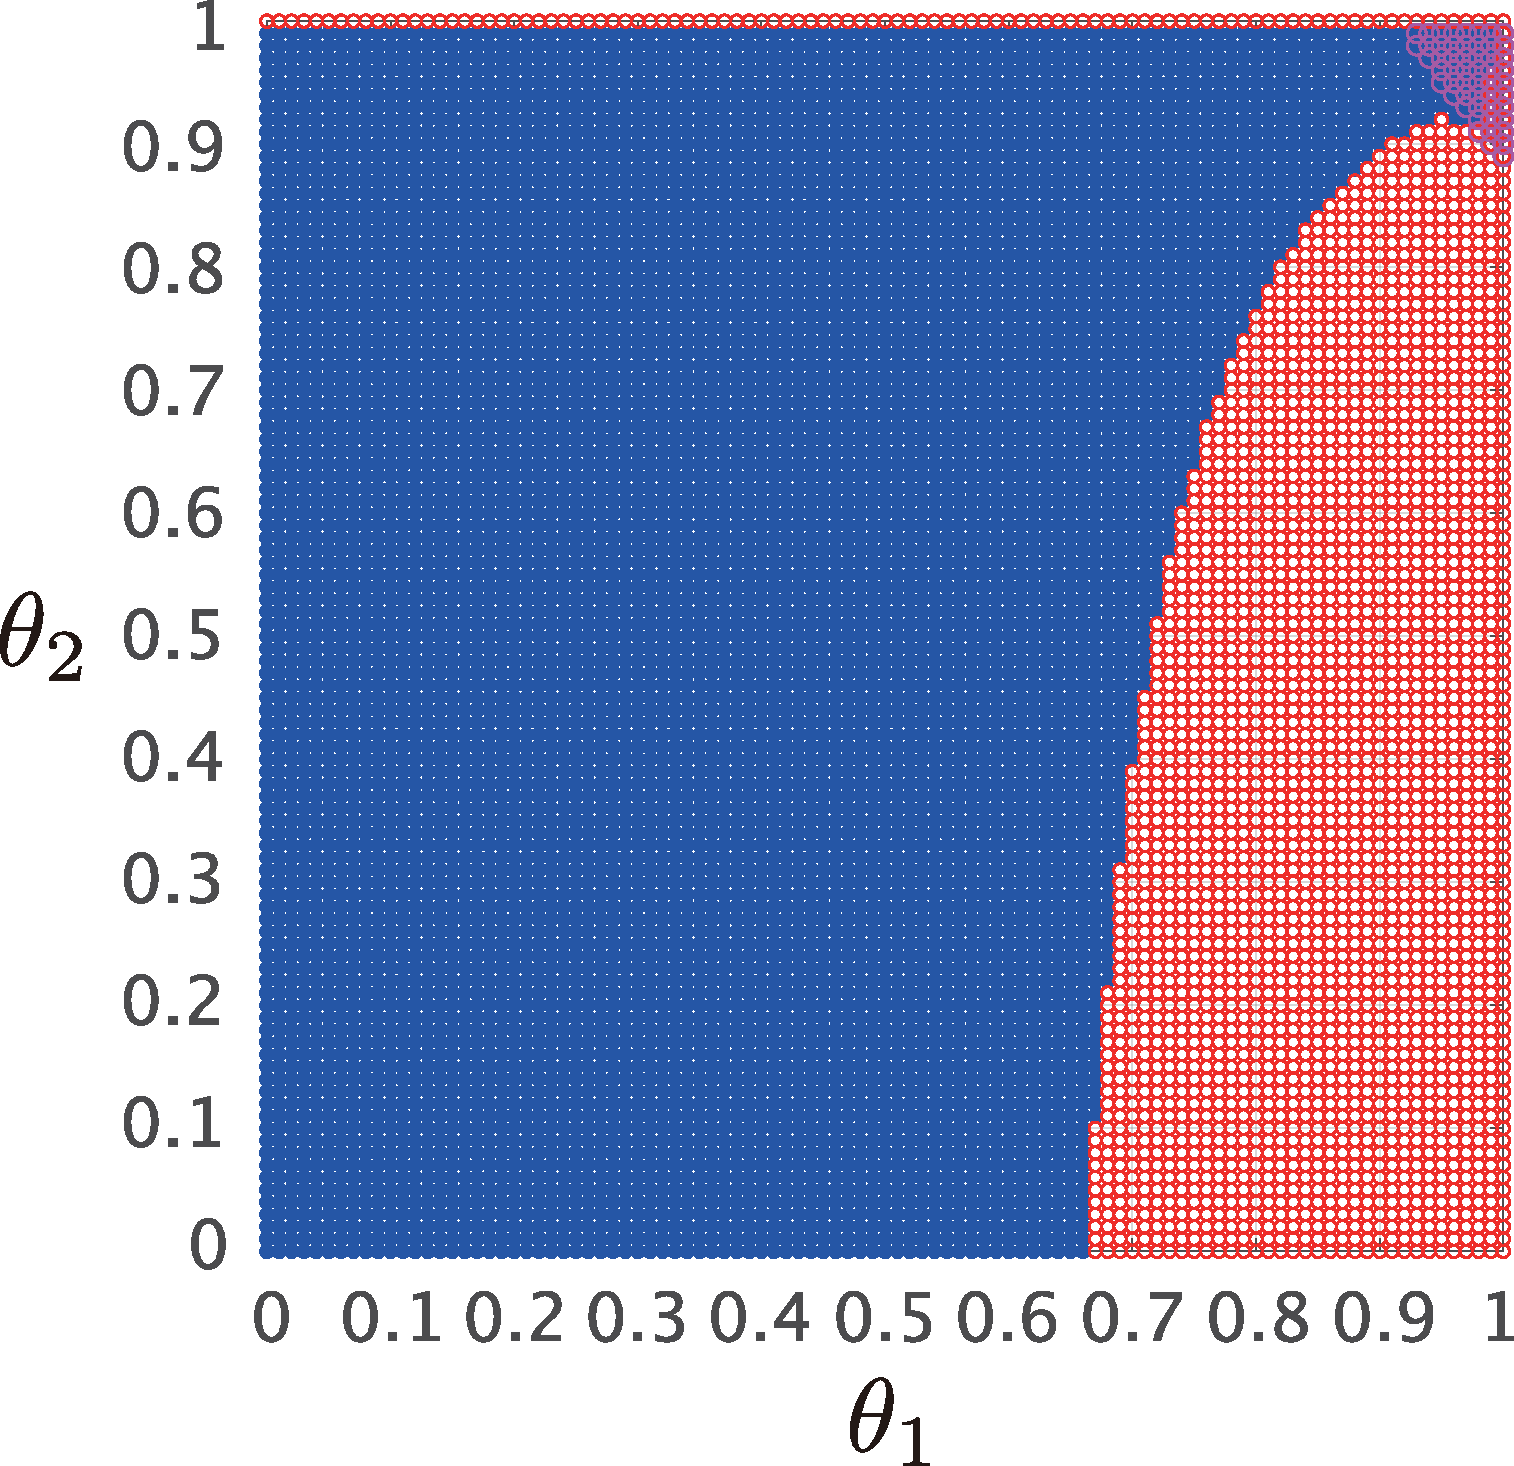
\includegraphics[width = .85\linewidth]{figs/gam01thm}
    \subcaption{ $\gamma=0.1$ }
  \end{minipage}
  \begin{minipage}{0.32\linewidth}
    \centering
    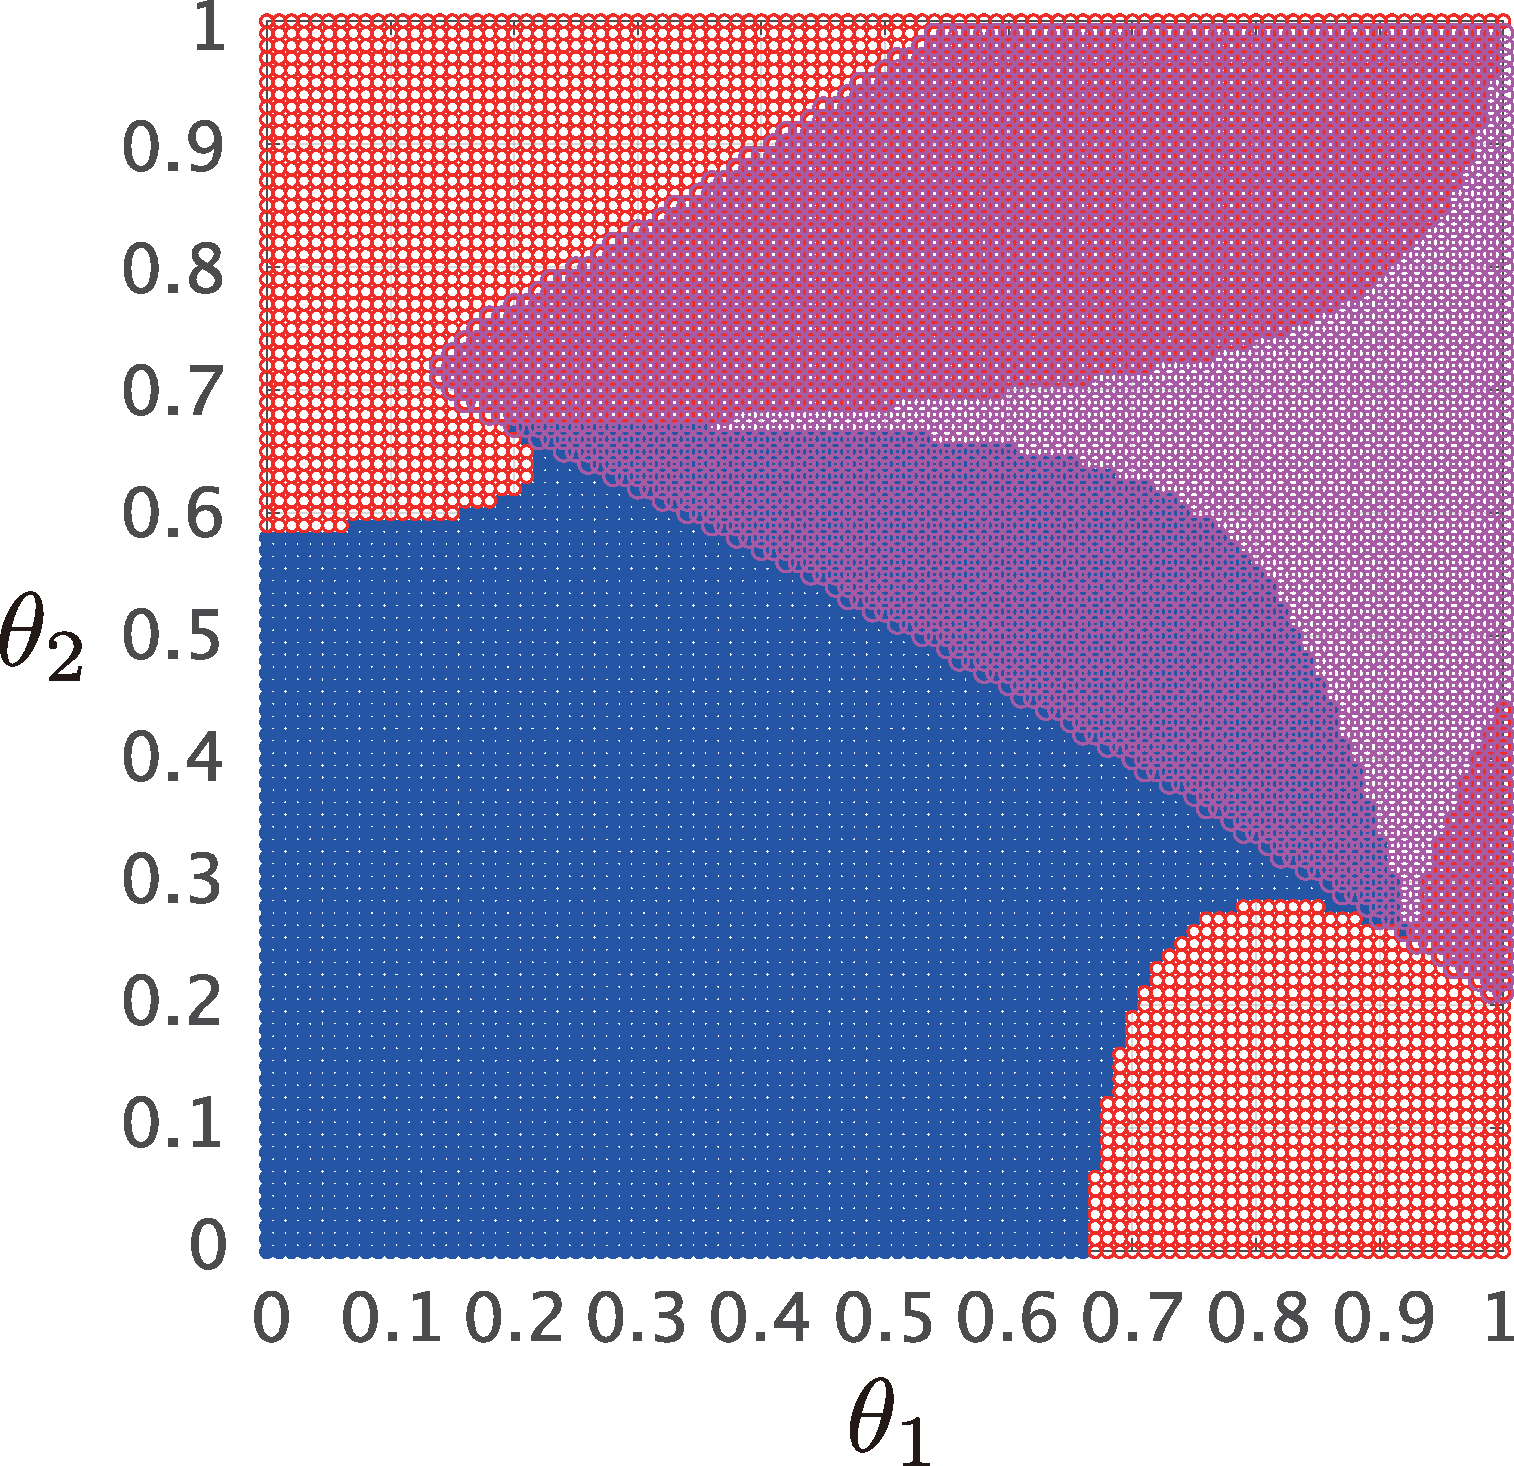
\includegraphics[width = .85\linewidth]{figs/gam2thm}
    \subcaption{ $\gamma=2$ }
  \end{minipage}
  \begin{minipage}{0.32\linewidth}
    \centering
    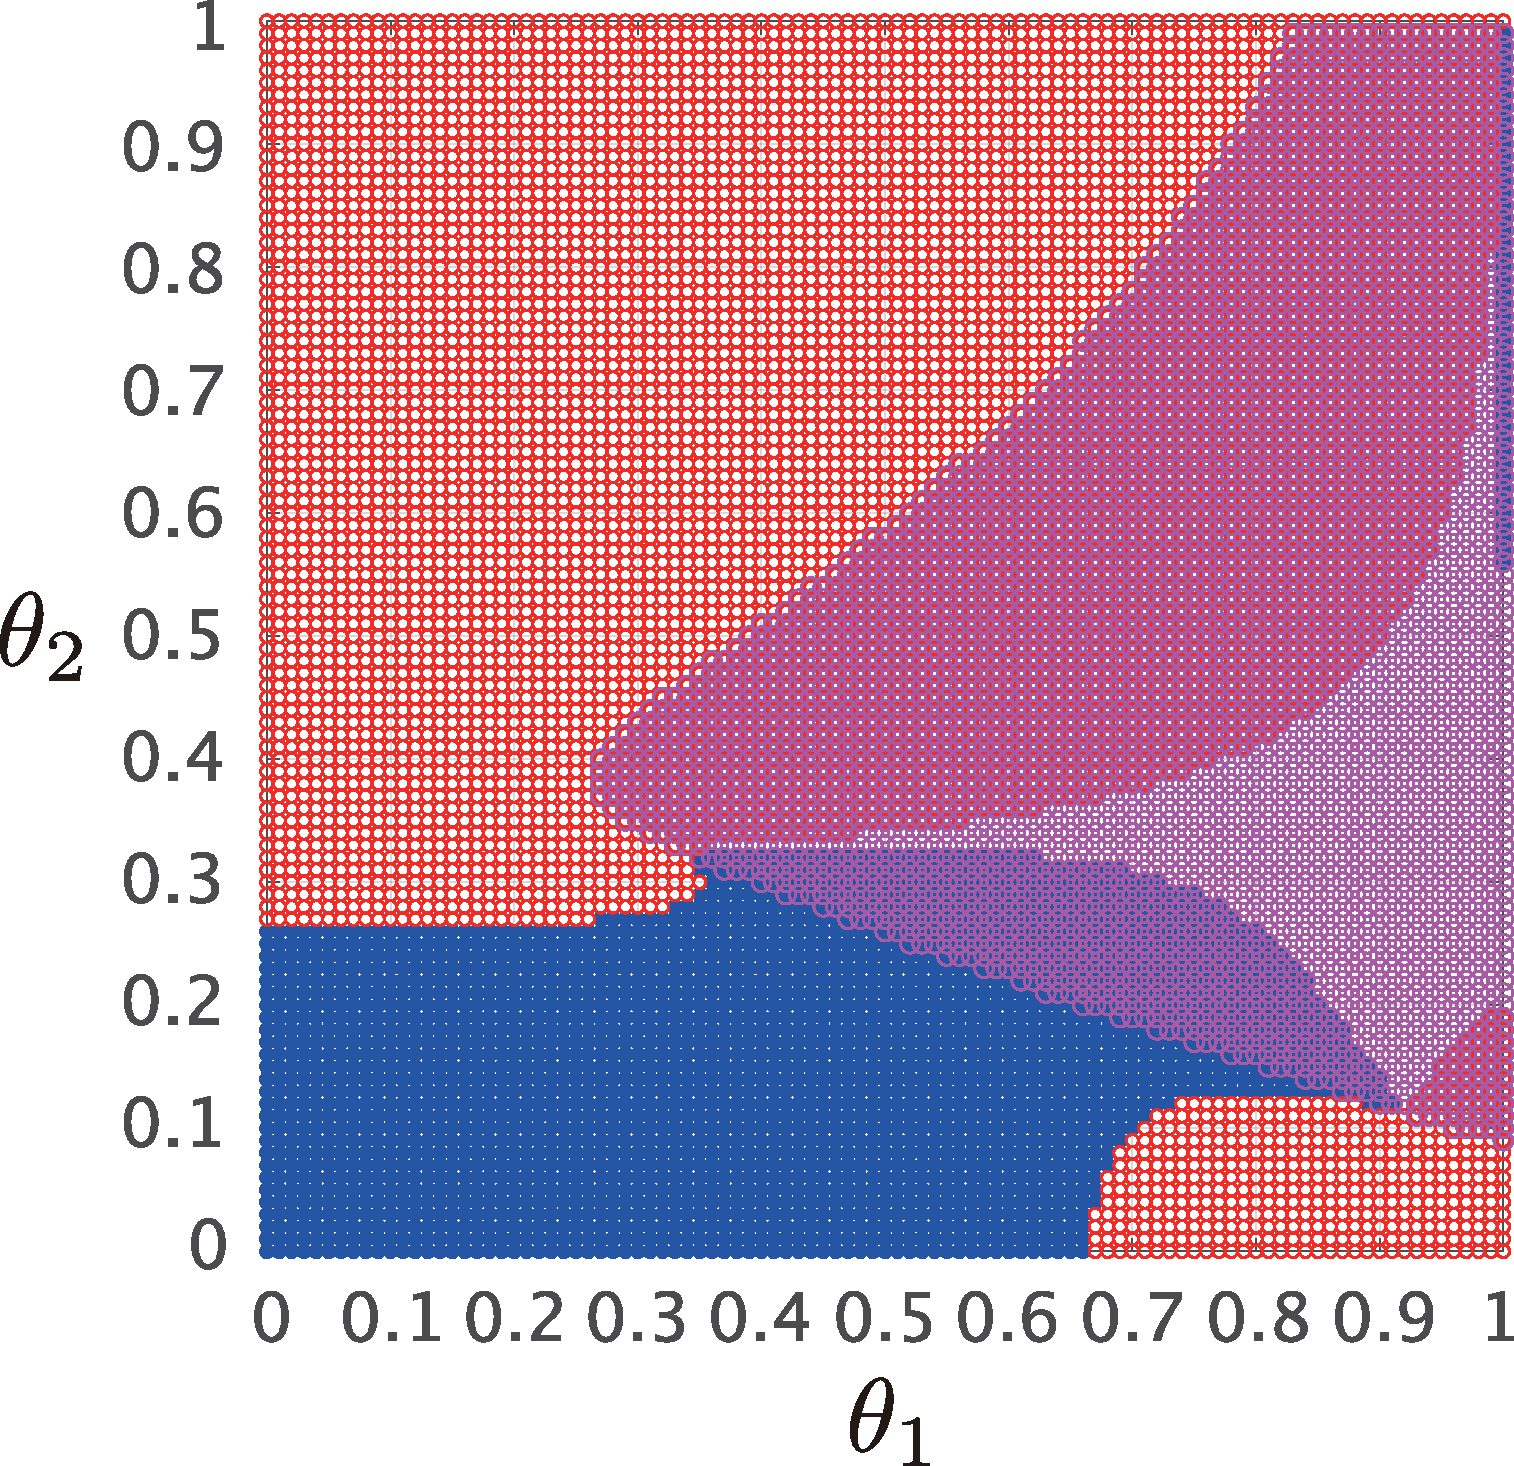
\includegraphics[width = .85\linewidth]{figs/gam5thm}
    \subcaption{ $\gamma=5$ }
  \end{minipage}
  \caption{例\ref{ex:linsyssim}の定数に対する近似線形モデルの同期解析}
  \label{fig:gamthm}
  }
\end{figure}

\begin{figure}[t]
  \centering
  {
  \begin{minipage}{0.32\linewidth}
    \centering
    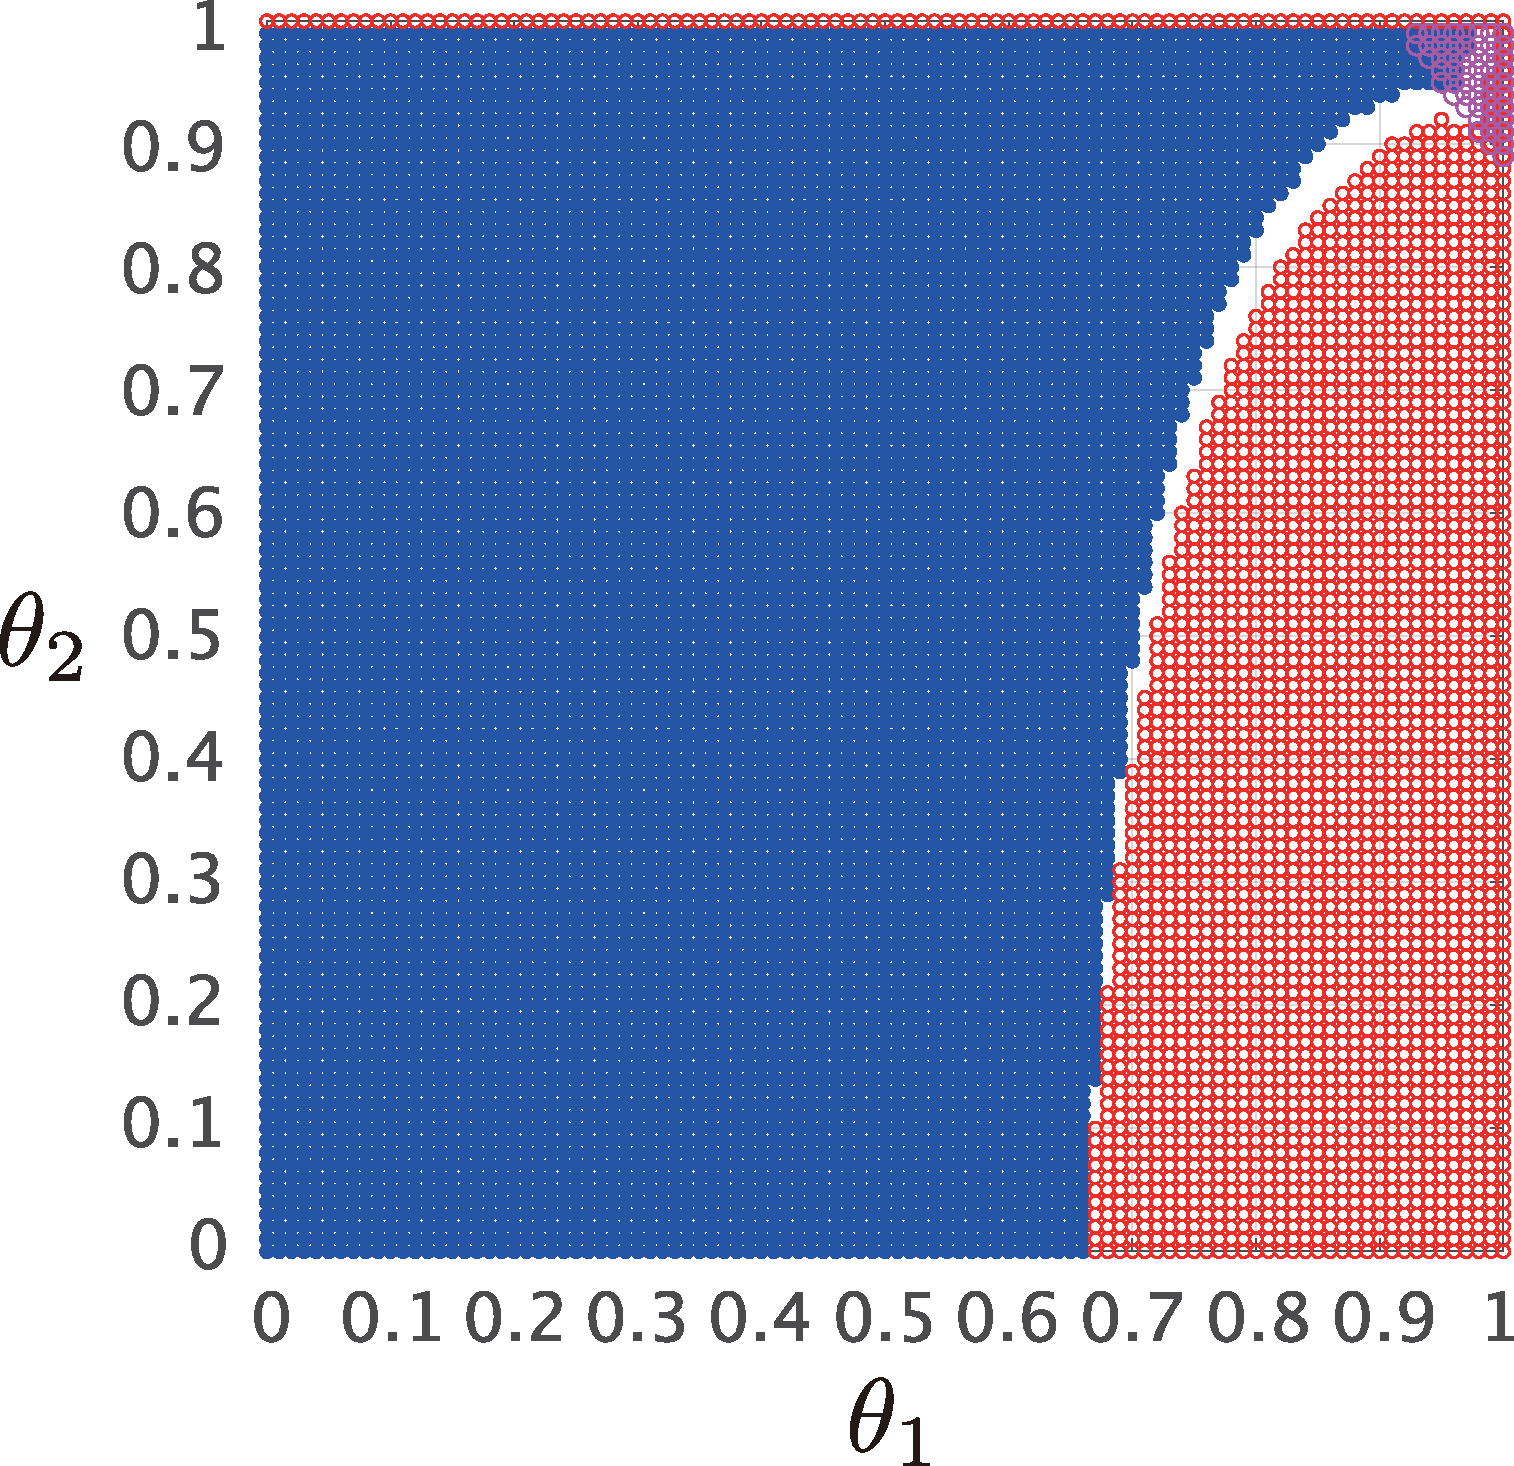
\includegraphics[width = .85\linewidth]{figs/gam01ex}
    \subcaption{ $\gamma=0.1$ }
  \end{minipage}
  \begin{minipage}{0.32\linewidth}
    \centering
    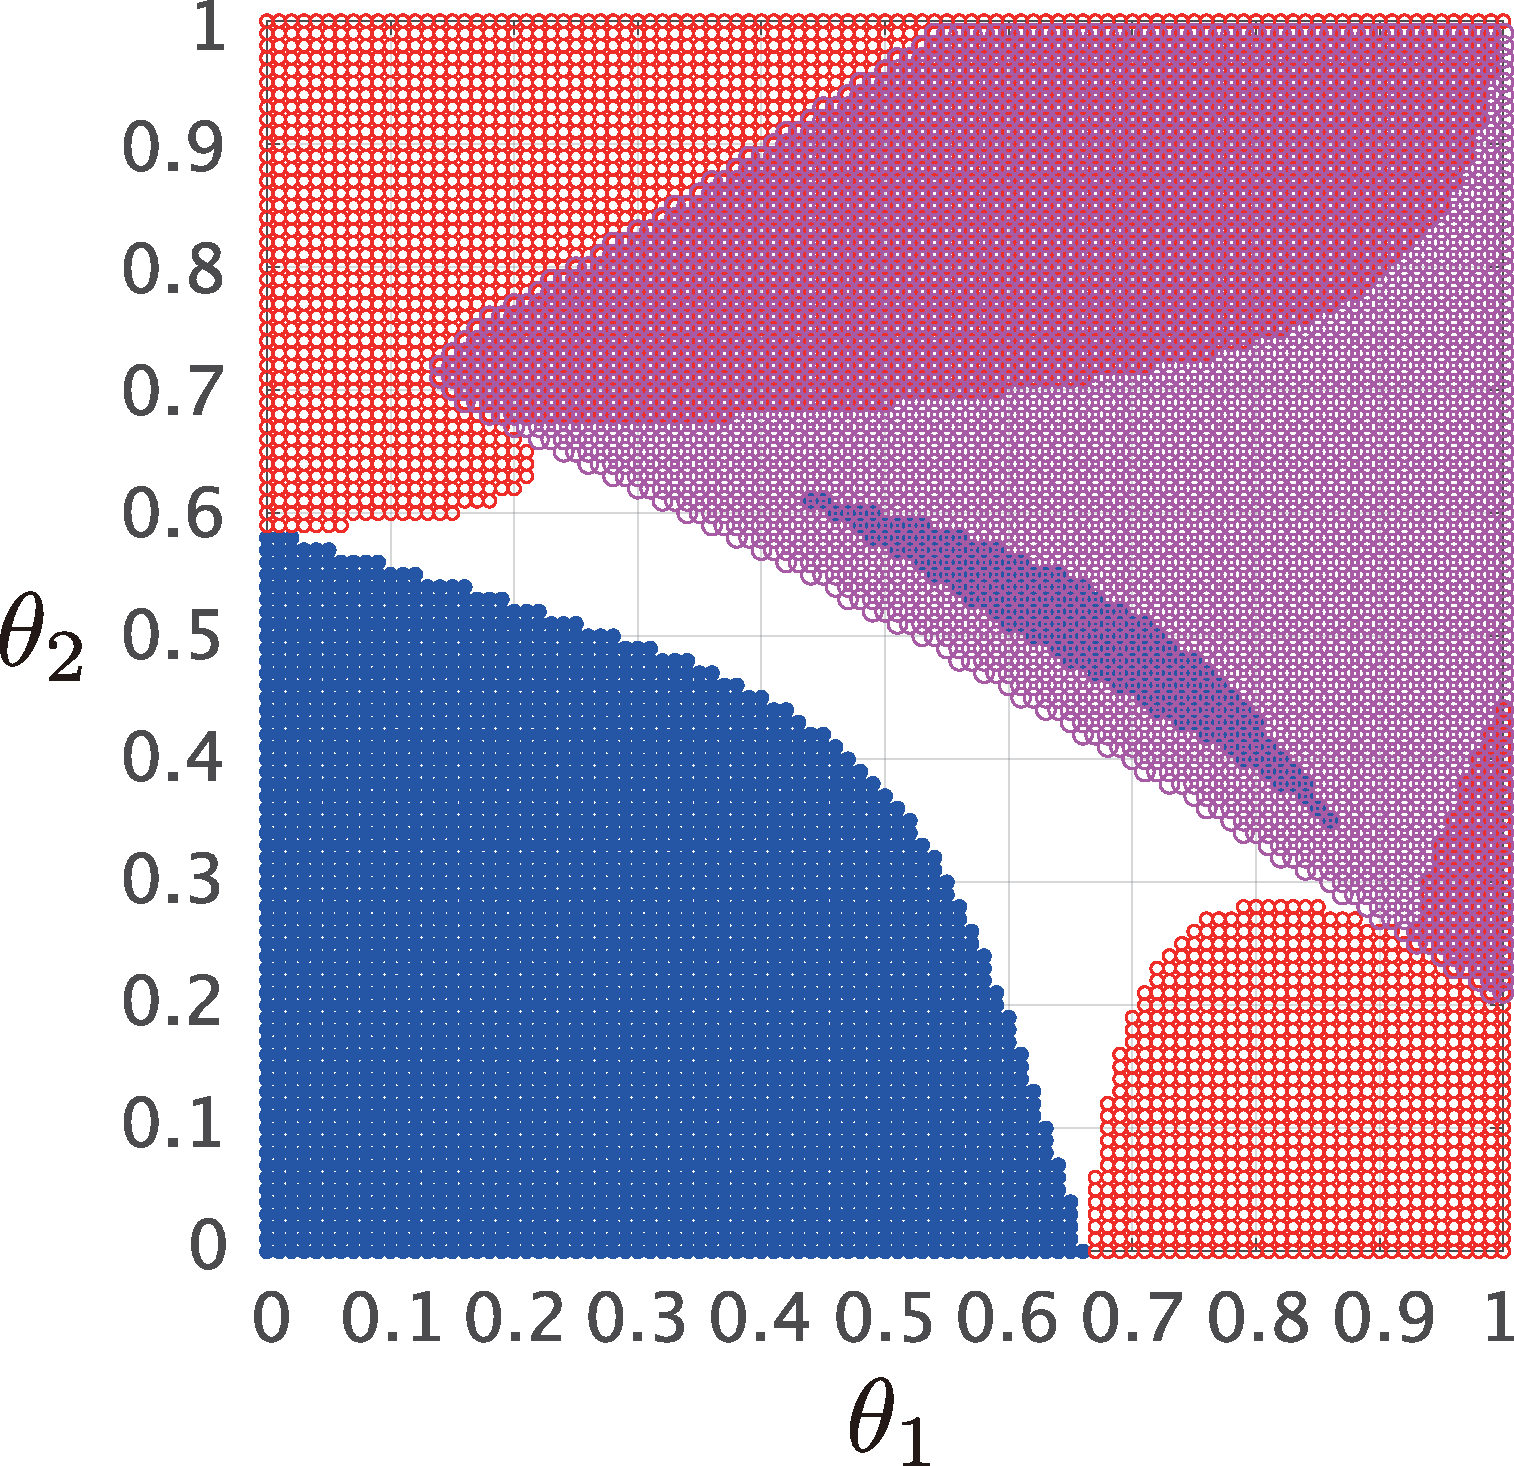
\includegraphics[width = .85\linewidth]{figs/gam2ex}
    \subcaption{ $\gamma=2$ }
  \end{minipage}
  \begin{minipage}{0.32\linewidth}
    \centering
    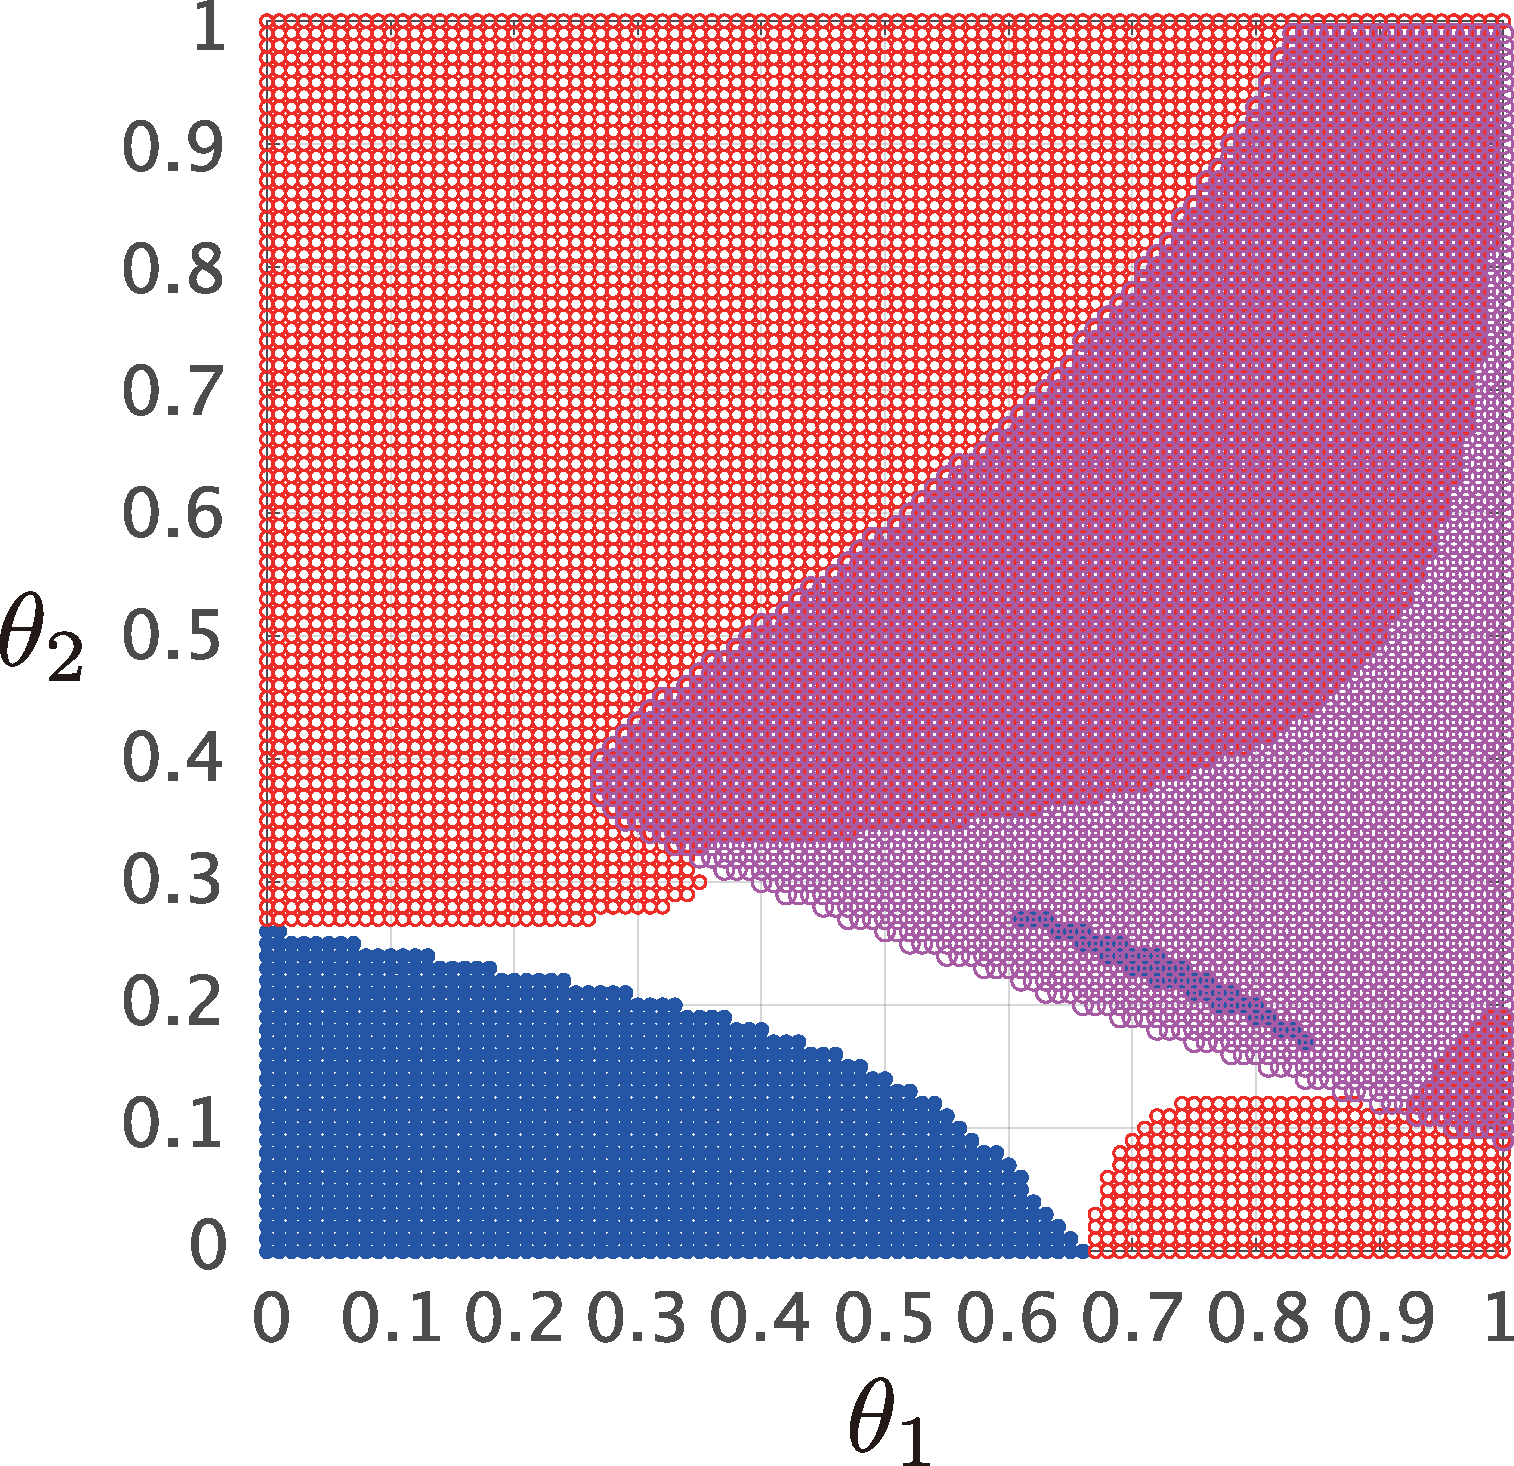
\includegraphics[width = .85\linewidth]{figs/gam5ex}
    \subcaption{ $\gamma=5$ }
  \end{minipage}
  \caption{定数の設定を変更した場合の近似線形モデルの同期解析}
  \label{fig:gamex}
  }
\end{figure}


\begin{例}[正実性や特異摂動近似に基づく近似線形モデルの同期解析]\label{ex:linthm}
定理\ref{thm:sync}を用いて,例\ref{ex:linsyssim}で扱った3つの発電機から構成される近似線形モデルの同期を解析してみよう。
発電機の物理定数などの設定はすべて例\ref{ex:linsyssim}と同じであるとする。
\ref{fig:gamsta}(a)--(c)に,定理\ref{thm:sync}で示される必要条件が満たされないパラメータの領域を重ねてプロットしたものが\ref{fig:gamthm}(a)--(c)である。
ただし,条件(i)と(ii)はすべてのパラメータに対して満たされていたため,条件(iii)について,$L-CA^{-1}B$の固有値に実部が負であるものが含まれる場合を赤で示し,複素数の固有値が含まれる場合を紫で示している。
この結果で注目すべき点はつぎの2つである。
\begin{itemize}
\item 赤で示されているパラメータ領域は,同期が達成される青いパラメータ領域の境界の一部を正確に捉えている。
\item 紫で示されているパラメータ領域は,同期が達成される青いパラメータ領域と重なる部分が存在している。
\end{itemize}
まず,1点目に関して,条件(iii)の必要条件は「システムが不安定化するような発電機の物理定数の設定が少なくとも1つは存在すること」を表していることに注意されたい。
したがって,例\ref{ex:linsyssim}で設定されている特定の定数に対しては,同期が達成されるパラメータ領域を必ずしも正確に捉えられるとは限らない。
一方で,実際に青い領域の境界の一部を正確に捉えられているという事実は,$L-CA^{-1}B$に実部が負の固有値が含まれる場合には,多くの場合で近似線形モデルが不安定となることを示唆している。
つぎに,2点目に関して,青の領域と紫の領域が重なっていることは,例\ref{ex:linsyssim}の物理定数の設定では同期が達成されている一方で,システムが不安定化するような他の定数が必ず存在することを意味している。
すなわち,青と紫が重なる領域は,発電機の物理定数などの値に依存して同期する場合としない場合が混在するパラメータ領域であるといえる。
なお,定理\ref{thm:sync}では,送電網が無損失であるとき,すなわち,$\theta_2=0$である横軸上のパラメータに対しては,赤ではない値に$\theta_1$を設定する限り,それらの定数の値に依らず近似線形モデルの同期が必ず達成されることも示されている。
一方で,定理\ref{thm:sync}により,定数に依存しない同期の達成を数学的に保証できるのは,この横軸上のパラメータのみであることに注意されたい。
それ以外のパラメータ領域における同期を数学的に解析するためには,「送電網が無損失である」という仮定からある程度の逸脱を許すように理論を一般化する必要がある。

参考として,定数の設定の一部を変更し
\begin{align*}
E_1^{\star}=2
,\quad
E_2^{\star}=4
,\quad
E_3^{\star}=6
,\quad
D_1 = 2
,\quad
D_2 = 1.5
,\quad
D_3 = 1
\end{align*}
とした場合の結果を\ref{fig:gamex}に示そう。
この図において現れている「白い領域」は,上記の定数の設定ではシステムが不安定である一方で,システムが不安定化するような定数が必ず存在することまでは数学的に証明されていないパラメータ領域である。
より具体的には,$L-CA^{-1}B$が非負の実数固有値しかもたないにも関わらず,近似線形モデルが何らかの理由で不安定化したパラメータ領域である。
このような,白い領域のパラメータ設定に対しては,他の定数を設定した場合に同期が達成されるか否かについて,以上の解析だけで結論を与えることはできない。
\end{例}

送電網が無損失でない場合に近似線形モデルの同期を特徴づける必要十分条件を導出することは難しい。
一方で,送電網が無損失であることが,式\ref{eq:trGs}の$G(s)$の正実性を特徴づける条件の1つであるという事実に基づいて,$G(s)$の正実な範囲からの逸脱を定量的に見積もることができれば,システムの同期が達成されるために発電機の物理定数などが満たすべき十分条件を求めることは可能である。


\section{非線形電力系統モデルの安定性解析\advanced}

\subsection{対象とする電力系統モデル}\label{sec:objmod}

第\ref{sec:stalin}節では,電力系統モデルが同期状態の近傍にあることを仮定して近似線形モデルを導出し,同期が達成されるための必要条件や十分条件を導出した。
本節では,システム制御理論における受動性という概念を用いることによって,非線形の微分代数方程式で記述される電力系統モデルに対しても同様の解析が可能であることを示す。
ただし,対象とする電力系統モデルはつぎの条件を満たすものと仮定する。

\begin{itemize}
\item 送電網は無損失であること,すなわち,式\ref{eq:Ypig}のアドミタンス行列$\bm{Y}$の実部は0であることを仮定する。
\item 電力系統に接続されている発電機は,式\ref{eq:gendynVI}で記述されるものとする。
ただし,$X_{{\rm d}i}'=X_{{\rm q}i}$を仮定する。
\item 発電機バスを除くすべてのバスには式\ref{eq:cpw}で記述される定電力の負荷が接続されているものとする。
\item 各発電機の機械的トルクと界磁電圧は,定常潮流状態においてすべての発電機の周波数偏差が0となるような定数に設定されているものとする。
\end{itemize}
まず,1点目の送電網の仮定については,数学的に電力系統モデルの同期を証明するためにはほとんど不可欠な仮定であるといえる。
実際,送電損失がある場合には,電力系統モデルの解析には数値的手法に頼らざるを得ないことが多くの文献で議論されている\cite{narasimhamurthi1984existence,yang2019distributed}。
また,第\ref{sec:stalin}節で示されているように,送電網は無損失であることは近似線形モデルが正実性をもつことの必要条件となっている。
なお,第\ref{sec:passstab}節で後述するように,線形システムの範疇では受動性と正実性の概念は数学的に等価であるため,受動性に基づく解析を行うためには不可欠な仮定といえる。

2点目,3点目については,発電機と負荷に対してどちらも標準的なモデルを仮定することを意味している。
なお,定インピーダンスの負荷が存在する場合には,第\ref{sec:modload}節で議論したクロン縮約により送電網のアドミタンス行列にあらかじめ組み込まれていると解釈することは可能である。
ただし,送電網が無損失であるためには,負荷のインピーダンスの実部も0でなければならないことに注意されたい。

4点目については,実際の電力系統制御では負荷の値や送電線のアドミタンスの値などをすべて正確に知ることはできないため,電力系統モデルが周波数偏差0の潮流状態を維持することが可能な,すなわち,需給バランスを維持することが可能な機械的トルクと界磁電圧の値が設定されていることは自明な仮定ではない。
しかしながら,本節で議論する電力系統モデルの受動性を利用することによって,未知の定数が電力系統モデルに含まれていたとしても,機械的トルクや界磁電圧を自動的に調整して漸近的に周波数偏差を0とするようなフィードバック制御機構を系統的に設計することが可能となる。
このことは,第??節で詳述する。

なお,第\ref{sec:powflow}節における潮流計算の議論からわかるように,需給バランスを達成する機械的トルクと界磁電圧の組み合わせは無数に存在する。
言い換えると,電力系統モデルの周波数偏差0の潮流状態は,各発電機の機械的トルクと界磁電圧に依存する関数となる。
したがって,その潮流状態が漸近的に達成されるための安定性解析では,潮流状態そのものが機械的トルクや界磁電圧の設定値に依存して変化することを前提にしなければならない。
この点についても後の議論で詳述する。

\subsection{受動性に基づく安定性解析}\label{sec:passstab}

\subsubsection{受動性の定義}

まずは,電力系統モデルに限らない,入力アフィンな非線形システムに対して受動性の概念を導入する。
入力$u$と出力$y$の次元がどちらも$m$であり,状態$x$の次元が$n\geq m$であるような動的システム
\begin{align}\label{eq:nlsig}
\Sigma: \simode{
\dot{x} &= f(x) + Bu \\
y &= h(x) + Du
}
\end{align}
を考える。
ただし,$f:\mathbb{R}^{n} \rightarrow \mathbb{R}^{n}$と$h:\mathbb{R}^{n} \rightarrow \mathbb{R}^{m}$は滑らかな関数であり,
\begin{align}\label{eq:fh0}
f(0)=0,\qquad
h(0)=0
\end{align}
を満たすものとする。
また,$B$と$D$は行列であるとする。
なお,関数$f(x)$と$g(x)$の滑らかさに関する条件は,システム$\Sigma$の解軌道$x(t)$が一意に定まることを保証するために課されるものであり,以降の議論で陽に用いることはない。
一方で,式\ref{eq:fh0}の条件は,$(x^{\star},u^{\star},y^{\star})=(0,0,0)$においてシステムが平衡することを意味している。
以下では,平衡点は$\star$を付して表記する。
ここで,システム$\Sigma$の安定性は,平衡点$x^{\star}=0$に対して,つぎのように定義される。

\begin{定義}[非線形システムの漸近安定性]\label{def:stabnl}
式\ref{eq:nlsig}のシステム$\Sigma$を考える。
原点を中心とする半径$\epsilon$の球の内部を
\begin{align*}
\mathcal{B}_{\epsilon} := \{
x \in \mathbb{R}^n : \|x\| < \epsilon
\}
\end{align*}
と表す。
任意の初期値$x_0 \in \mathcal{B}_{\epsilon}$に対して$\Sigma$の解軌道$x(t)$が0に収束するような,ある$\epsilon>0$が存在するとき,$\Sigma$の平衡点$x^{\star}=0$は\emph{漸近安定}であると呼ぶ。
ただし,入力は恒等的に0とする。
\end{定義}

定義\ref{def:difsta}における線形システムに対する安定性では,議論の対象とする平衡点を陽に指定する必要はなく,初期値に関する球領域$\mathcal{B}_{\epsilon}$を考える必要もなかった。
これは,線形システムの場合には,初期値の球の大きさに依らず,球内の任意の初期値に対して,その解軌道がある1つの平衡点に収束するのであれば,その平衡点は原点のみであることが示されるためである。
一方で,非線形システムの場合には,平衡点が1つであるとは限らず,\emph{安定領域}の大きさ,すなわち,解軌道が平衡点に収束する初期値の領域の大きさも平衡点によって異なる。
なお,ある平衡点が漸近安定であることは,その平衡点近傍で導出された近似線形モデルが漸近安定であることと等価である。
しかしながら,近似線形モデルに基づく解析によって平衡点の漸近安定性が示されたとしても,その解析の結果として平衡点の安定領域の大きさを見積もることはできない。
したがって,その安定領域の大きさに関して何らかの有益な知見を得ることが,非線形システムを直接的に解析する場合の目的の1つとなる。


以降の議論のため,式\ref{eq:nlsig}のシステム$\Sigma$において,議論の対象とする入力$u$の集合を$\mathcal{U}\subseteq \mathbb{R}^m$,状態$x$の集合を$\mathcal{X} \subseteq \mathbb{R}^n$と表す。
また,これらの入力と状態の集合から作られる出力$y$の集合を$\mathcal{Y} \subseteq \mathbb{R}^n$と表す。
なお,これらの集合は第??節において安定領域の大きさを議論する際に用いるが,その他の箇所では$\mathcal{X}$を$\mathbb{R}^n$,$\mathcal{U}$と$\mathcal{Y}$を$\mathbb{R}^m$と読み替えても構わない。
この記法のもとで,システム$\Sigma$の受動性をつぎのように導入する。

\begin{定義}[非線形システムの受動性]\label{def:passive}
式\ref{eq:nlsig}のシステム$\Sigma$に対して,$W(0)=0$であり,かつ,任意の$u \in \mathcal{U}$に対して
\begin{align}\label{eq:conpv}
\frac{d}{dt} W\bigl( x(t) \bigr) \leq u^{\sf T} y
,\qquad
t \geq 0
\end{align}
を満たす微分可能な正定値関数$W:\mathcal{X} \rightarrow \mathbb{R}_{\geq 0}$が存在するとき,$\Sigma$は\emph{受動的}であると呼ぶ。
特に,上記の正定値関数$W$に加えて
\begin{align}\label{eq:conosp}
\frac{d}{dt} W\bigl( x(t) \bigr) \leq u^{\sf T} y -\rho\|y\|^2
,\qquad
t \geq 0
\end{align}
を満たすある定数$\rho >0$が存在するとき,$\Sigma$は\emph{強受動的}であると呼ぶ。
\end{定義}

定義\ref{def:passive}における正定値関数$W(x)$は一般に\emph{蓄積関数}(storage function)と呼ばれている。
蓄積関数の時間微分は,システム$\Sigma$の解軌道$x(t)$に沿った微分であり,微分の連鎖律を用いて
\begin{align*}
\frac{d}{dt} W\bigl( x(t) \bigr)
= \nabla W^{\sf T} (x) \frac{dx}{dt} = \nabla W^{\sf T} (x) 
\bigl( 
f(x) + Bu
\bigr)
\end{align*}
と計算される。
ただし,$\nabla W:\mathcal{X} \rightarrow \mathbb{R}^n$は$W(x)$の勾配関数を表しており
\begin{align*}
\nabla W(x) := \sfcol \left( 
\frac{\partial }{\partial x_i}W(x)
\right)
\end{align*}
で定義される。
なお,式\ref{eq:conosp}を満たすシステムは\emph{出力強受動的}(output strictly passive)であると呼ぶべきものであるが,本書では単に強受動的であると表記する。
また,文献によっては,式\ref{eq:conosp}右辺の$\rho\|y\|^2$の代わりに,より一般的な正定値関数$\rho(y)$を用いて強受動性を定義している場合もある。
\red{文献を挙げたい}

線形システムの範疇では,システムの受動性は,その伝達関数の正実性と等価であることが知られている。
実際,補題\ref{lem:prlem}に示される正定行列$P$が存在するならば,蓄積関数を$W(x)=\frac{1}{2}x^{\sf T}Px$と選ぶことにより,式\ref{eq:conpv}の不等式が満たされる。
この事実は,以下のように簡単に確認できる。
まず,蓄積関数の時間微分は
\begin{align*}
\frac{d}{dt} W\bigl( x(t) \bigr)
&=(Px)^{\sf T}(Ax+Bu) \\
&= 
\frac{1}{2}
\left\{
x^{\sf T} (A^{\sf T} P +PA)x 
+ u^{\sf T} B^{\sf T}Px+ x^{\sf T} PBu
\right\}
\end{align*}
となる。
ただし,任意のベクトル$v$,$w$および行列$M$に対して,
\[
v^{\sf T}Mw = \frac{1}{2} (v^{\sf T}Mw + w^{\sf T}M^{\sf T}v)
\]
であることを用いた。
このとき,式\ref{eq:conpv}の不等式は
\begin{align*}
\mat{x\\u}^{\sf T}
\mat{
A^{\sf T} P +PA & B^{\sf T}P-C \\
PB-C^{\sf T} & - (D+D^{\sf T})
}
\mat{x\\u}
\leq 0
\end{align*}
と書き換えられることから,補題\ref{lem:prlem}の正定な$P$が存在するならば,任意の$x$と$u$に対してこの不等式が成り立つことがわかる。
逆に,式\ref{eq:conpv}の不等式を満たす$W(x)$が存在するとき,システムの伝達関数が正実であることも示される。
証明は\cite[第5.9.1節]{antoulas2005approximation}などを参照されたい。

\begin{例}[並列された安定な1次系の受動性]\label{ex:psF}
式\ref{eq:Fss}の線形システム$F$が強受動的であることを確かめてみよう。
以下では,表記の簡単化のため,式\ref{eq:Fss}の状態と入出力に対する添字$f$は省略する。
例\ref{ex:Fspr2}で示されているように,式\ref{eq:prlem}の行列不等式の解は$P=\omega_0 \sfdiag(M_i)$により与えられる。
この事実に基づき,蓄積関数を
\begin{align*}
W(x)= \frac{\omega_0}{2}
x^{\sf T}
\sfdiag(M_i)
x
\end{align*}
と選ぶ。
この蓄積関数の勾配関数は
\begin{align}\label{eq:nabWo}
\nabla W(x) = \omega_0 \sfdiag(M_i) x
\end{align}
であることから,蓄積関数の時間微分に対して
\begin{align}\label{eq:exFps}
\spliteq{
\frac{d}{dt} W \bigl( x(t) \bigr)
&= 
\omega_0  x^{\sf T} \sfdiag(M_i)
\left\{
-\sfdiag \left( 
\frac{D_i}{ M_i} 
\right)x + 
\sfdiag \left( 
\frac{1}{ M_i} 
\right)
u
\right\} \\
& \leq 
y^{\sf T} u
- \frac{\sfmin \left\{ D_i \right\}}{\omega_0}
\|y \|^2
}
\end{align}
が成り立つことがわかる。
\end{例}

\red{強受動をFDIの円条件で説明する?KYP補題が必要。消散性についても付録とかで補足しておく?}

\subsubsection{受動性に基づくフィードバック系の安定性解析}

以下では,受動性の概念を用いることによって,第\ref{sec:stalin}節で説明された伝達関数の正実性に関する事実と同等の事実が,非常に簡潔に導出できることを確認する。
これらの理解にはリアプノフの安定理論の基礎的な知識が前提となるため,必要に応じて\red{付録??}を参照されたい。

式\ref{eq:conpv}において,入力が恒等的に0である場合の解軌道$x(t)$を考えると
\begin{align*}
\frac{d}{dt} W\bigl( x(t) \bigr) \leq 0
,\qquad
t \geq 0
\end{align*}
となることから,受動的なシステムに対する蓄積関数が原点の平衡点の安定性を示すリアプノフ関数となることは明らかである。
ただし,この事実により結論づけられる安定性は,原点を含むある有界な領域の中に解軌道が留まることだけを意味しており,解軌道が原点の平衡点に収束することまでは一般に示されない。
一方で,より強い条件を満たす強受動的なシステムに対しては,つぎの事実が成り立つ。

\begin{補題}[強受動的なシステムの漸近安定性]\label{lem:pssta}
式\ref{eq:nlsig}のシステム$\Sigma$が強受動的であり,かつ,入力が恒等的に0であるとき
\begin{align}\label{eq:zeroso}
h\bigl(
x(t)
\bigr)=0,\qquad
\forall t\geq 0
\end{align}
が成り立つ解軌道が$x(t)=0$のみであるならば,$\Sigma$の平衡点$x^{\star}=0$は漸近安定である。
\end{補題}

\begin{証明}
\red{リアプノフとラサールが必要}
\end{証明}

補題\ref{lem:pssta}に示されるように,強受動的なシステムの原点の平衡点は漸近安定である。
ただし,原点に留まる平衡軌道とは別に,式\ref{eq:zeroso}が成り立つような解軌道$x(t)$が存在する場合には,その解軌道が原点の平衡点に収束するか否かはこの議論だけではわからない。
この補足的な条件は,\emph{零状態可観測性}と呼ばれるものであり,線形システムに対しては標準的な可観測性と等価である。
なお,本書で扱う電力系統モデルの解析では,恣意的なパラメータ設定を行わない限り,この零状態可観測性は常に満たされるものと考えて差し支えない。


つぎの事実は,\emph{受動定理}と呼ばれるものであり,正実性に関する補題\ref{lem:prpre}を受動性の観点で記述し,非線形システムを含む場合に一般化したものと解釈できる。

\begin{figure}[t]
  \centering
  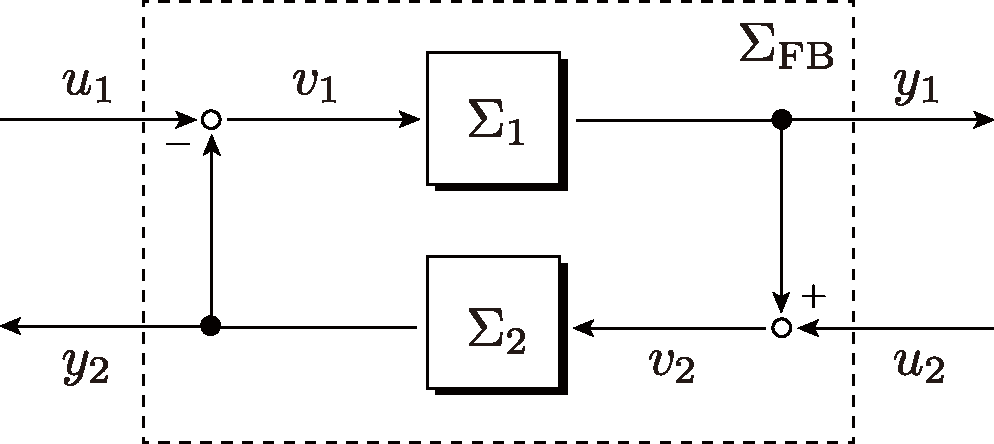
\includegraphics[width = .50\linewidth]{figs/fbnlin}
  \caption{ネガティブ・フィードバック系}
  \label{fig:stasig12}
\end{figure}

\begin{定理}[受動定理]\label{thm:psthm}
\ref{fig:stasig12}に示されるシステム$\Sigma_1$と$\Sigma_2$のネガティブ・フィードバック系$\Sigma_{\rm FB}$を考える。
このとき,$\Sigma_1$が入力$v_1$,出力$y_1$に関して受動的であり,かつ,$\Sigma_2$が入力$v_2$,出力$y_2$に関して受動的であるならば,$\Sigma_{\rm FB}$は入力$(u_1,u_2)$,出力$(y_1,y_2)$に関して受動的である。
特に,$\Sigma_1$が前述の入出力に関して強受動的であるならば,$\Sigma_{\rm FB}$は入力$u_1$,出力$y_1$に関して強受動的である。
さらに,$\Sigma_1$と$\Sigma_2$がどちらも前述の入出力に関して強受動的であるならば,$\Sigma_{\rm FB}$は入力$(u_1,u_2)$,出力$(y_1,y_2)$に関して強受動的である。
\end{定理}

\begin{証明}
まず,$\Sigma_1$と$\Sigma_2$がどちらも強受動的である場合を考える。
システム$\Sigma_i$の入力$v_i$,出力$y_i$に関する蓄積関数を$W_i(x_i)$とする。
このとき,それらの蓄積関数の和に関して
\begin{align*}
\frac{d}{dt}\bigl(W_1(x_1) + W_2(x_2) \bigr) \leq v_1^{\sf T}y_1 + v_2^{\sf T}y_2 
- \rho_1 \|y_1\|^2 - \rho_2 \|y_2\|^2
\end{align*}
が成り立つ。
この不等式に,$v_1=u_1 -y_2$と$v_2=u_2 +y_1$の関係を代入すれば
\begin{align*}
\frac{d}{dt}\bigl(W_1(x_1) + W_2(x_2) \bigr) \leq \mat{u_1^{\sf T} & u_2^{\sf T} }\mat{y_1\\y_2} 
-\rho_{0} 
\left\|
\mat{
y_1\\
y_2
}
\right\|^2
\end{align*}
が得られる。
ただし,$\rho_{0}:=\sfmin \{\rho_1,\rho_2\}$である。
したがって,ネガティブ・フィードバック系の入力$(u_1,u_2)$,出力$(y_1,y_2)$に関する蓄積関数を$W_1(x_1)+W_2(x_2)$と構成できることがわかる。
この議論において,$u_2=0$,$\rho_2=0$とすれば,$\Sigma_1$のみが強受動的である場合の題意が示される。
また,$\rho_1=\rho_2=0$とすれば,$\Sigma_1$と$\Sigma_2$が受動的である場合の題意が示される。
\end{証明}

定理\ref{thm:psthm}の証明に示されているように,フィードバック系の蓄積関数は,結合された2つのシステムの蓄積関数の和として構成することができる。
このように,システムの受動性を示すことができれば,システムが線形であるか非線形であるかを意識することなく,簡潔にフィードバック系の安定性を解析することができる。
なお,結合されるシステムの平衡点が原点である場合には,フィードバック系の平衡点も原点となることは容易に確かめられる。
また,定理\ref{thm:psthm}では,$\Sigma_1$のみが強受動的である場合を考えているが,$\Sigma_2$のみが強受動的である場合も同様である。
3つ以上のシステムが結合される場合にも,同様の解析が可能である\cite{moylan1978stability}。

受動性を用いた安定性解析を行う場合には,「対象とするシステムが受動的か否かを判定すること」が最も重要な課題となる。
そのためには,システムの受動性を示す蓄積関数を構成することが必要である。
しかしながら,特に非線形システムに対しては,構成可能な蓄積関数の形式は一般に明らかではないため,対象とするシステムがもつ物理的な性質などを巧みに利用して,発見的に蓄積関数を見つけ出す必要がある。
なお,電力系統モデルに対しては,発電機の運動エネルギーや電圧のポテンシャルなどから構成されるエネルギー関数が蓄積関数となることが知られている。
このことは,第\ref{sec:psanpw}節で後述する。

\subsubsection{平衡点に依存しない受動性}

これまでの議論では,原点が平衡点であることを前提にしていた。
しかしながら,電力系統モデルの平衡状態は,電力の消費と供給がバランスするような状態であるため,解析の対象となる平衡点ではシステムの内部状態は0とはならない。
さらに,その平衡状態そのものが機械的トルクや界磁電圧の設定値に依存して変化するため,個々の平衡状態の選択に依存することなくシステムの受動性を議論することが望ましい。
このような状況を扱うために提唱された概念が,\emph{平衡点に依存しない受動性}(equilibrium-independent passivity)と呼ばれるものである\cite{hines2011equilibrium,simpson2019equilibrium}。
なお,文献によっては,\emph{シフトされた受動性}(shifted passivity)とも呼ばれている\cite{monshizadeh2019conditions}.
その定義はつぎのように与えられる。

\begin{定義}[平衡点に依存しない受動性]\label{def:eipassive}
式\ref{eq:nlsig}のシステム$\Sigma$を考える。
定常的な入力によって実現可能な平衡点の集合を
\begin{align}\label{eq:asbleq}
\mathcal{E}_{\Sigma} :=
\left\{
x^{\star} \in \mathcal{X}: 
\mbox{$0 = f(x^{\star})+B u^{\star}$を満たす$u^{\star}\in \mathcal{U}$が存在する}
\right\}
\end{align}
と表す。
各々すべての平衡点$x^{\star} \in \mathcal{E}_{\Sigma}$に対して,$W_{x^{\star}} (x^{\star})=0$であり,かつ,任意の$u \in \mathcal{U}$に対して
\begin{align}\label{eq:eiconpv}
\frac{d}{dt} W_{x^{\star}} \bigl( x(t) \bigr) \leq (u-u^{\star})^{\sf T} (y-y^{\star})
,\qquad
t \geq 0
\end{align}
を満たす微分可能な正定値関数$W_{x^{\star}}:\mathcal{X} \rightarrow \mathbb{R}_{\geq 0}$が存在するとき,$\Sigma$は\emph{平衡点に依らず受動的}であると呼ぶ。
ただし,$x^{\star}$における定常的な入力と出力を
\begin{align}\label{eq:uystar}
\spliteq{
u^{\star} &:= -(B^{\sf T}B)^{-1}B^{\sf T}f(x^{\star}),
\\
y^{\star} &:= h(x^{\star}) - D (B^{\sf T}B)^{-1}B^{\sf T}f(x^{\star})
}
\end{align}
と表している。
特に,上記の正定値関数$W_{x^{\star}}(x)$に加えて
\begin{align}\label{eq:eiconosp}
\frac{d}{dt} W_{x^{\star}} \bigl( x(t) \bigr) \leq (u-u^{\star})^{\sf T} (y-y^{\star})
-\rho\|y-y^{\star}\|^2
,\qquad
t \geq 0
\end{align}
を満たすある定数$\rho >0$が存在するとき,$\Sigma$は\emph{平衡点に依らず強受動的}であると呼ぶ。
\end{定義}

定義\ref{def:eipassive}では,システムの平衡点$x^{\star} \in \mathcal{E}_{\Sigma}$を基準としてその受動性が定義されていると解釈できる。
ただし,注目する平衡点は1つではなく,定常的な入力に対して実現可能な「各々すべての平衡点」に対する受動性が条件として課されていることに注意されたい。
原点に平衡点をもつシステムに対して定義\ref{def:passive}の意味での受動性が示されたとしても,それ以外の平衡点での受動性が必ずしも示されるとは限らない。
したがって,標準的な受動性と比較して,定義\ref{def:eipassive}ではより強い条件が課されている。
なお,線形システムの範疇では,システムが零固有値をもたない限り,これらの受動性の定義は等価である\cite{hines2011equilibrium}。
この事実を簡単な例を用いて確認してみよう。

\begin{例}[並列された安定な1次系の平衡点に依らない受動性]\label{ex:eipsF}
例\ref{ex:psF}で示されているように,式\ref{eq:Fss}の線形システム$F$は強受動的である。
この事実に基づいて,$F$が平衡点に依らず強受動的であることを確かめてみよう。
例\ref{ex:psF}と同様に,各変数の添字$f$は省略して表記する。
任意に選ばれた平衡点$x^{\star} \in \mathcal{E}_F$に対して,蓄積関数を
\begin{align*}
W_{x^{\star}}(x)= \frac{\omega_0}{2}
(x -x^{\star})^{\sf T}
\sfdiag(M_i)
(x -x^{\star})
\end{align*}
と選ぶ。
この蓄積関数の勾配関数は
\begin{align}\label{eq:nabW}
\nabla W_{x^{\star}}(x) = \omega_0 \sfdiag(M_i) (x -x^{\star})
\end{align}
であることから,蓄積関数の時間微分に対して
\begin{align}\label{eq:tdsys1}
\spliteq{
\frac{d}{dt} W_{x^{\star}} \bigl( x(t) \bigr) 
&= 
\omega_0 (x -x^{\star})^{\sf T} \sfdiag(M_i) \times \\
&\hspace{3em} \left\{
-\sfdiag \left( 
\frac{D_i}{ M_i} 
\right)x + 
\sfdiag \left( 
\frac{1}{ M_i} 
\right)
u
\right\}
\\
&= 
\omega_0 (x -x^{\star})^{\sf T} \sfdiag(M_i) \times \\
&\hspace{3em} \left\{
-\sfdiag \left( 
\frac{D_i}{ M_i} 
\right) (x -x^{\star}) + 
\sfdiag \left( 
\frac{1}{ M_i} 
\right)
(u -u^{\star})
\right\}
\\
& \leq \textstyle
(y -y^{\star})^{\sf T}(u -u^{\star})
- \frac{\sfmin \left\{ D_i \right\}}{\omega_0}
\|y -y^{\star}\|^2
}
\end{align}
が成り立つことがわかる。
この計算は,2つ目の等号に対して
\begin{align*}
0=-\sfdiag \left( 
\frac{D_i}{ M_i} 
\right)x^{\star} + \sfdiag \left( 
\frac{1}{ M_i} 
\right)u^{\star}
\end{align*}
を用いたこと以外は,式\ref{eq:exFps}と全く同じである。
\end{例}

例\ref{ex:eipsF}において注目すべき点の1つは,式\ref{eq:nabW}の勾配関数$\nabla W_{x^{\star}}(x)$が,式\ref{eq:nabWo}の勾配関数$\nabla W(x)$を用いて
\begin{align*}
\nabla W_{x^{\star}}(x) = \nabla W(x) - \nabla W(x^{\star})
\end{align*}
のように,平衡点における勾配との差分の形式で表せることである。
この表現から逆算して蓄積関数を求めると
\begin{align}\label{eq:paraW}
W_{x^{\star}}(x) = W(x) - W(x^{\star}) - \nabla^{\sf T} W(x^{\star}) (x-x^{\star})
\end{align}
となる。
興味深いことに,システムが平衡点に依らず受動的である場合には,その蓄積関数は必ず式\ref{eq:paraW}の形式で書き表せることが文献\cite{simpson2019equilibrium}において示されている。
なお,例\ref{ex:eipsF}で示された線形システムのように蓄積関数が2次形式である場合には,$W_{x^{\star}}(x)=W(x-x^{\star})$であるが,一般の非線形関数に対してはこの等式は成り立たない。

定義\ref{def:eipassive}では,式\ref{eq:paraW}の蓄積関数$W_{x^{\star}}(x)$が正定値関数であることが条件として課されている。
すなわち
\begin{align*}
W(x) - W(x^{\star})  > \nabla^{\sf T} W(x^{\star}) (x-x^{\star})
,\qquad
\forall x\neq x^{\star},
 \quad
x \in \mathcal{X}
,\quad
x^{\star} \in \mathcal{E}_{\Sigma}
\end{align*}
でなければならない。
この不等式は,$W_{x^{\star}}(x)$が平衡点を除く定義域$\mathcal{X}$において狭義凸関数(\red{付録??})であることを意味している。
この事実からわかるように,蓄積関数$W_{x^{\star}}(x)$が凸であるような状態の領域$\mathcal{X}$が,平衡点に依存しない受動性を用いた安定性解析に重要な役割を果たす。
なお,凸関数である$W(x)$に対して,式\ref{eq:paraW}右辺は$x$と$x^{\star}$の$W(x)$に関する\emph{ブレグマン距離}(Bregman distance)と呼ばれている。


平衡点に依存しない受動性による安定性解析はつぎの事実にもとづく。
証明は補題\ref{lem:pssta}と同様である。

\begin{補題}[平衡点に依らず強受動的なシステムの漸近安定性]\label{lem:eipssta}
式\ref{eq:nlsig}のシステム$\Sigma$が平衡点に依らず強受動的であり,かつ,各々すべての平衡点$x^{\star} \in \mathcal{E}_{\Sigma}$に対して,入力が恒等的に$u^{\star}$であるとき
\begin{align}\label{eq:eizeroso}
h\bigl(
x(t)
\bigr) + D u^{\star}= y^{\star},\qquad
\forall t\geq 0
\end{align}
が成り立つ解軌道が$x(t)=x^{\star}$のみであるならば,$\Sigma$の平衡点$x^{\star}=0$は漸近安定である。
ただし,$u^{\star}$と$y^{\star}$は式\ref{eq:uystar}により定義される。
\end{補題}

定理\ref{thm:psthm}に相当する事実も以下のように示される。
\ref{fig:stasig12}に示されネガティブ・フィードバック系$\Sigma_{\rm FB}$に対して,その平衡点において満たされるべき方程式は
\begin{align}\label{eq:eqfb}
\simode{
0 = f_1 (x_1^{\star}) + B_1 \bigl( u_1^{\star} - h_2(x_2^{\star}) \bigr)\\
0 = f_2 (x_2^{\star}) + B_2 \bigl( u_2^{\star} + h_1(x_1^{\star}) \bigr)
}
\end{align}
である。
ただし,$\Sigma_1$と$\Sigma_2$の変数は添字により区別している。
定常的な入力によって実現可能な平衡点の集合を
%\begin{align*}
%\mathcal{E}_{\Sigma_{\rm FB}}:=
%\left\{
%(x_1^{\star},x_2^{\star})\in \mathcal{E}_{\Sigma_1} \times \mathcal{E}_{\Sigma_2}:
%\mbox{式\ref{eq:eqfb}を満たす$(u_1^{\star},u_2^{\star}) \in \mathcal{U}_1 \times \mathcal{U}_2$
%が存在する}
%\right\}
%\end{align*}
\begin{align*}
\mathcal{E}_{\Sigma_{\rm FB}}:=
\left\{
(x_1^{\star},x_2^{\star})\in \mathcal{E}_{\Sigma_1} \times \mathcal{E}_{\Sigma_2}: \!\!
\mbox{$\begin{array}{l}
\mbox{式\ref{eq:eqfb}を満たす$(u_1^{\star},u_2^{\star}) \in \mathcal{U}_1 \times \mathcal{U}_2$ }
\vspace{-1mm} \\
\mbox{が存在する}
\end{array}$
}\!\!\!
\right\}
\end{align*}
と表すとき,$\Sigma_{\rm FB}$の平衡点に依らない受動性はこの平衡点集合$\mathcal{E}_{\Sigma_{\rm FB}}$に関して定義される。
ただし,平衡点$(x_1^{\star},x_2^{\star})$における定常的な
入力$(u_1^{\star},u_2^{\star})$と
出力$(y_1^{\star},y_2^{\star})$は,
式\ref{eq:uystar}と同様に定義する。
ここで,$\Sigma_1$と$\Sigma_2$がどちらも平衡点に依らず受動的であり,かつ,少なくともどちらか一方が強受動的であるならば,与えられた$(u_1^{\star},u_2^{\star})$に対して,式\ref{eq:eqfb}を満たす$(x_1^{\star},x_2^{\star})$が一意に定まることが知られている\cite{simpson2019equilibrium}。
これらの記法のもと,つぎの結果が得られる。
証明は定理\ref{thm:psthm}と同様である。

\begin{定理}[平衡点に依らない受動性に関する受動定理]\label{thm:eipsthm}
\ref{fig:stasig12}に示されるシステム$\Sigma_1$と$\Sigma_2$のネガティブ・フィードバック系$\Sigma_{\rm FB}$を考える。
このとき,$\Sigma_1$が入力$v_1$,出力$y_1$に関して平衡点に依らず強受動的であり,かつ,$\Sigma_2$が入力$v_2$,出力$y_2$に関して平衡点に依らず受動的であるならば,$\Sigma_{\rm FB}$は入力$u_1$,出力$y_1$に関して平衡点に依らず強受動的である。
特に,$\Sigma_1$と$\Sigma_2$がどちらも前述の入出力に関して強受動的であるならば,$\Sigma_{\rm FB}$は入力$(u_1,u_2)$,出力$(y_1,y_2)$に関して平衡点に依らず強受動的である。
\end{定理}


\subsection{電力系統モデルの受動性解析}\label{sec:psanpw}

\subsubsection{電力系統モデルの定式化}

本節では,電力系統モデルが平衡点に依らない受動性をもつことを示す。
第\ref{sec:objmod}節で前述したように,送電網は無損失であることを仮定し,式\ref{eq:Ypig}のアドミタンス行列を
\begin{align*}
\bm{Y}=\bm{j}B
\end{align*}
と表す。
このとき,式\ref{eq:ohmY}と式\ref{eq:defPQVIi}の関係を用いれば,バス$i$に機器から供給される有効電力と無効電力は
\begin{align}\label{eq:powbal}
\spliteq{
P_i &= \sum_{j\neq i}^{N} B_{ij} |\bm{V}_i| |\bm{V}_j| \sfsin(\angle \bm{V}_i -\angle \bm{V}_j),
\\
Q_i &= - B_{ii} |\bm{V}_i|^2 -
\sum_{j\neq i}^{N} B_{ij} |\bm{V}_i| |\bm{V}_j| \sfcos(\angle \bm{V}_i -\angle \bm{V}_j)
}
\end{align}
と表せる。
ただし,$B_{ij}$は$B$の$(i,j)$要素を表す。
なお,式\ref{eq:powbal}の等式がすべてのバスで成り立つことは,式\ref{eq:ohmY}の連立方程式が満たされることと等価であることに注意されたい。


発電機が接続されているバスの添字集合を$\mathcal{I}_{\rm G}$と表し,負荷が接続されているバスの添字集合を$\mathcal{I}_{\rm L}$と表す。
ただし,$|\mathcal{I}_{\rm G}| + |\mathcal{I}_{\rm L}| =N$である。
第\ref{sec:objmod}節で前述したように,発電機バスの各$i \in \mathcal{I}_{\rm G}$に対しては
\begin{subequations}\label{eq:modgnld}
\begin{align}\label{eq:modgnlda}
\simode{
\dot{\delta}_i&= \omega_0  \Delta \omega_i\\
M_i   \Delta \dot{\omega}_i&= 
- D_i \Delta\omega_i  
- P_i
+P_{{\rm mech}i}
\\
\tau_{{\rm d}i} \dot{E}_i & = 
 -\frac{X_{{\rm d}i}}{X_{{\rm q}i}}E_i
+\left(
\frac{X_{{\rm d}i}}{X_{{\rm q}i}}-1
\right)
|\bm{V}_i| \sfcos (\delta_i - \angle \bm{V}_i ) 
+ V_{{\rm field}i}
}
\end{align}
の微分方程式に従う発電機モデルが接続されているものとする。
ただし,界磁電圧$V_{{\rm field}i}$は定数であるものとし,各$i \in \mathcal{I}_{\rm G}$に供給される有効電力と無効電力は
\begin{align}\label{eq:modgnldb}
\spliteq{
P_i &= \frac{E_i |\bm{V}_i|}{X_{{\rm q}i}} \sfsin (\delta_i - \angle \bm{V}_i),
\\
Q_i &= \frac{E_i |\bm{V}_i|}{X_{{\rm q}i}} \sfcos (\delta_i - \angle \bm{V}_i)
-\frac{|\bm{V}_i|^2}{X_{{\rm q}i}},
}
\end{align}
である。
また,負荷バスの各$i \in \mathcal{I}_{\rm L}$に対しては
\begin{align}\label{eq:modgnldc}
P_i = P_{{\rm load}i}
,\qquad
Q_i = Q_{{\rm load}i}
\end{align}
\end{subequations}
で表される定電力の負荷モデルが接続されているものとする。
ただし,$P_{{\rm load}i}$と$Q_{{\rm load}i}$は負荷からバスに供給される有効電力と無効電力を表す定数であり,消費を表す場合はそれらの符号は負である。

\subsubsection{電力系統モデルの受動性}

受動性に基づく安定性解析のため,電力系統モデルを2つのサブシステムのフィードバック系として解釈することを考える。
1つ目のサブシステムは,発電機の機械的な動特性を表す
\begin{align}\label{eq:sys1}
\mathds{F}_i:
\simode{
M_i \Delta \dot{\omega}_i&= 
- 
D_i
\Delta\omega_i  
 + 
v_{\mathds{F}_i}
\\
y_{\mathds{F}_i}&= \omega_0 \Delta\omega_i  
}
\end{align}
である。
すべての発電機バス$i \in \mathcal{I}_{\rm G}$に対して,$\mathds{F}_i$をまとめたサブシステムを$\mathds{F}$と表す。
2つ目のサブシステムは,発電機の励磁系の動特性や送電網におけるバス電圧フェーザの方程式などをまとめた
\begin{subequations}\label{eq:sys2G}
\begin{align}\label{eq:sys2}
\mathds{G}_i : 
\simode{
\dot{\delta}_i &= v_{\mathds{G}_i}
\\
\tau_{{\rm d}i} \dot{E}_i & = 
 -\frac{X_{{\rm d}i}}{X_{{\rm q}i}}E_i
+\left(
\frac{X_{{\rm d}i}}{X_{{\rm q}i}}-1
\right)
|\bm{V}_i| \sfcos (\delta_i - \angle \bm{V}_i ) 
+ V_{{\rm field}i}
\\
y_{\mathds{G}_i}&= \frac{E_i |\bm{V}_i|}{X_{{\rm q}i}} \sfsin (\delta_i - \angle \bm{V}_i)
}
\end{align}
である。
この$ \mathds{G}_i $は発電機バス$i \in \mathcal{I}_{\rm G}$に関するサブシステムであるが,式\ref{eq:sys2}におけるバスの電圧フェーザは,発電機バス$i \in \mathcal{I}_{\rm G}$に関する連立方程式
\begin{align}\label{eq:gVeq}
\simode{
\frac{E_i |\bm{V}_i|}{X_{{\rm q}i}} \sfsin (\delta_i - \angle \bm{V}_i) &=
\sum_{j\neq i}^{N} B_{ij} |\bm{V}_i| |\bm{V}_j| \sfsin(\angle \bm{V}_i -\angle \bm{V}_j)
\\
\frac{E_i |\bm{V}_i|}{X_{{\rm q}i}} \sfcos (\delta_i - \angle \bm{V}_i)
&-\frac{|\bm{V}_i|^2}{X_{{\rm q}i}} = \\
- B_{ii} |\bm{V}_i|^2 
& -\sum_{j\neq i}^{N} B_{ij} |\bm{V}_i| |\bm{V}_j| \sfcos(\angle \bm{V}_i -\angle \bm{V}_j)
}
\end{align}
と負荷バス$i \in \mathcal{I}_{\rm L}$に関する連立方程式
\begin{align}\label{eq:lVeq}
\simode{
&P_{{\rm load}i} =
\sum_{j\neq i}^{N} B_{ij} |\bm{V}_i| |\bm{V}_j| \sfsin(\angle \bm{V}_i -\angle \bm{V}_j)
\\
&Q_{{\rm load}i} = 
- B_{ii} |\bm{V}_i|^2 -
\sum_{j\neq i}^{N} B_{ij} |\bm{V}_i| |\bm{V}_j| \sfcos(\angle \bm{V}_i -\angle \bm{V}_j)
}
\end{align}
\end{subequations}
を満たさなければならない。
したがって,すべての$i \in \mathcal{I}_{\rm G}$に対して,式\ref{eq:sys2}から式\ref{eq:lVeq}をまとめたものをひとつのサブシステムとみなし,それを$\mathds{G}$と表す。
これらのサブシステム$\mathds{F}$,$\mathds{G}$は
\begin{align}
v_{\mathds{F}_i} = P_{{\rm mech}i}- y_{\mathds{G}_i}
,\qquad
v_{\mathds{G}_i} = y_{\mathds{F}_i}
,\qquad
i \in \mathcal{I}_{\rm G}
\end{align}
というネガティブ・フィードバックにより結合される。

以下では,すべての$i \in \mathcal{I}_{\rm G}$に対して,$v_{{\mathds F}_i}$や$P_{{\rm mech}i}$などをまとめたベクトルを添え字$i$を除いた記号で表す。
なお,$|\bm{V}|$と$\angle \bm{V}$に関しては,発電機バスと負荷バスのすべての電圧フェーザ変数をまとめたベクトルとする。
ここで,式\ref{eq:sys1}を式\ref{eq:Fss}と比較することにより,$\mathds{F}$と$F$の入出力関係が等しいことがわかる。
また,例\ref{ex:eipsF}から示されるように,$\mathds{F}$は入力$v_{\mathds F}$,出力$y_{\mathds F}$に関して平衡点に依らず強受動的である。
したがって,式\ref{eq:sys2}の$\mathds{G}$が入力$v_{\mathds G}$,出力$y_{\mathds G}$に関して平衡点に依らず受動的であるならば,定理\ref{thm:eipsthm}および受動性が出力の正定数倍に関して不変であるという事実から,電力系統モデルは入力$P_{\rm mech}$,出力$\Delta \omega$に関して平衡点に依らず強受動的であることが導かれる。
これに関して,つぎの事実が示される。

\begin{補題}[励磁系と送電網に関するポテンシャル関数]\label{lem:volpot}
式(\ref{eq:sys2G})のシステム$\mathds{G}$に対して,ポテンシャル関数を
\begin{align}\label{eq:potWx}
\spliteq{
&W_0(\delta, E; |\bm{V}|, \angle \bm{V}) \\
&\hspace{1em} :=  \sum_{i=1}^{N}
\left\{
- \frac{1}{2} B_{ii} |\bm{V}_i|^2 
- \sum_{j\neq i}^{N} B_{ij} |\bm{V}_i| |\bm{V}_j| \sfcos(\angle \bm{V}_i -\angle \bm{V}_j)
\right\} \\
&\hspace{1em} + \sum_{i\in \mathcal{I}_{\rm G}}
\left\{
\frac{X_{{\rm d}i}}{2X_{{\rm q}i}(X_{{\rm d}i} - X_{{\rm q}i} )}  E_i^2
- 
\frac{E_i |\bm{V}_i|}{X_{{\rm q}i}} \sfcos (\delta_i - \angle \bm{V}_i)
+\frac{|\bm{V}_i|^2}{2X_{{\rm q}i}}
\right\}
\\
&\hspace{1em} +\sum_{i\in \mathcal{I}_{\rm L}}
\left\{
- P_{{\rm load}i} \angle \bm{V}_i
- Q_{{\rm load}i} \ln{|\bm{V}_i|}
\right\}
}
\end{align}
と定義する。
すべての$i\in \mathcal{I}_{\rm G} \cup \mathcal{I}_{\rm L}$に対して$|\bm{V}_i|\neq 0$であるとき
\begin{subequations}\label{eq:patW}
\begin{align}\label{eq:patWa}
\spliteq{
\frac{\partial W_0}{\partial |\bm{V}_i| } &= 0,
\\
\frac{\partial W_0}{\partial \delta_i} &= y_{\mathds{G}_i}
}
\spliteq{
\frac{\partial W_0}{\partial \angle \bm{V}_i } &= 0,
\\
\frac{\partial W_0}{\partial E_i} &= \frac{V_{{\rm field}i} - \tau_{{\rm d}i}\dot{E}_i  }{X_{{\rm d}i} - X_{{\rm q}i} },
}
\qquad
i\in \mathcal{I}_{\rm G}
\end{align}
および
\begin{align}
\frac{\partial W_0}{\partial |\bm{V}_i| } = 0
,\quad
\frac{\partial W_0}{\partial \angle \bm{V}_i } = 0
,\qquad i\in \mathcal{I}_{\rm L}
\end{align}
\end{subequations}
が成り立つ。
\end{補題}

\begin{証明}
まず,$\delta_i$と$E_i$に関する偏微分は
\begin{align*}
\frac{\partial W_0}{\partial \delta_i} &= \frac{E_i |\bm{V}_i|}{X_{{\rm q}i}} \sfsin (\delta_i - \angle \bm{V}_i) ,
\\
\frac{\partial W_0}{\partial E_i} &= - \frac{1}{X_{{\rm d}i} - X_{{\rm q}i}}
\left\{
-\frac{X_{{\rm d}i}}{X_{{\rm q}i}}E_i
+\left(
\frac{X_{{\rm d}i}}{X_{{\rm q}i}}-1
\right)
|\bm{V}_i| \sfcos (\delta_i - \angle \bm{V}_i ) 
\right\}
\end{align*}
となる。
したがって,式\ref{eq:sys2}から,式\ref{eq:patWa}の表現が得られる。
また,$i\in \mathcal{I}_{\rm G}$に対して
\begin{align*}
\spliteq{
\frac{\partial W_0}{\partial |\bm{V}_i| } &= 
- B_{ii} |\bm{V}_i|^2 
-
\sum_{j\neq i}^{N} B_{ij} |\bm{V}_i| |\bm{V}_j| \sfcos(\angle \bm{V}_i -\angle \bm{V}_j)
\\
&\hspace{13em} 
-\left(
\frac{E_i }{X_{{\rm q}i}} \sfcos (\delta_i - \angle \bm{V}_i)
-\frac{|\bm{V}_i|}{X_{{\rm q}i}}
\right)
\\
\frac{\partial W_0}{\partial \angle \bm{V}_i } &= 
B_{ij} |\bm{V}_i| |\bm{V}_j| \sfsin(\angle \bm{V}_i -\angle \bm{V}_j)
-
\frac{E_i |\bm{V}_i|}{X_{{\rm q}i}} \sfsin (\delta_i - \angle \bm{V}_i) 
}
\end{align*}
が得られる。
したがって,式\ref{eq:gVeq}から,これらが0であることがわかる。
同様に,$i\in \mathcal{I}_{\rm L}$に対して
\begin{align*}
\spliteq{
\frac{\partial W_0}{\partial |\bm{V}_i| } &= 
- B_{ii} |\bm{V}_i|^2 -
\sum_{j\neq i}^{N} B_{ij} |\bm{V}_i| |\bm{V}_j| \sfcos(\angle \bm{V}_i -\angle \bm{V}_j)
 - \frac{Q_{{\rm load}i}}{|\bm{V}_i|}
\\
\frac{\partial W_0}{\partial \angle \bm{V}_i } &= 
B_{ij} |\bm{V}_i| |\bm{V}_j| \sfsin(\angle \bm{V}_i -\angle \bm{V}_j)
-
P_{{\rm load}i}
}
\end{align*}
が得られる。
したがって,これらも0であることが,式\ref{eq:lVeq}からわかる。
\end{証明}

式(\ref{eq:sys2G})の$\mathds{G}$は微分代数方程式系として記述されているが,第\ref{sec:genmod}節や第\ref{sec:modload}節で議論されているように,バスの電圧フェーザ変数
$(|\bm{V}|,\angle \bm{V})$はクロン縮約を介することにより,発電機の状態変数$(\delta,E)$の関数とみなせる。
ただし,上述のような定電力の負荷モデルの場合には,それらを状態変数の陽な関数として書き下すことは難しいため,形式的に式(\ref{eq:sys2G})の微分代数方程式系を発電機の内部状態に関する常微分方程式系とみなすものとする。
このとき,式\ref{eq:potWx}のポテンシャル関数は
\begin{align}\label{eq:stops0}
W(\delta,E):= W_0\bigl( \delta,E; |\bm{V}|(\delta,E), \angle \bm{V}(\delta,E)  \bigr)
\end{align}
と表せる。
なお,補題\ref{lem:volpot}の結果から
\begin{align*}
\spliteq{
\frac{\partial W}{\partial \delta_i} &=
\frac{\partial W_0}{\partial \delta_i}
+
\sum_{j=1}^{N}
\left\{
\frac{\partial W_0}{\partial |\bm{V}_j|} 
\frac{\partial |\bm{V}_j|}{\partial \delta_i} 
+
\frac{\partial W_0}{\partial \angle \bm{V}_j} 
\frac{\partial \angle \bm{V}_j }{\partial \delta_i} 
\right\}
=
y_{\mathds{G}_i}
\\
\frac{\partial W}{\partial E_i} &=
\frac{\partial W_0}{\partial E_i}
+
\sum_{j=1}^{N}
\left\{
\frac{\partial W_0}{\partial |\bm{V}_j|} 
\frac{\partial |\bm{V}_j|}{\partial E_i} 
+
\frac{\partial W_0}{\partial \angle \bm{V}_j} 
\frac{\partial \angle \bm{V}_j }{\partial E_i} 
\right\}
=
\frac{V_{{\rm field}i} - \tau_{{\rm d}i}\dot{E}_i  }{X_{{\rm d}i} - X_{{\rm q}i} }
}
\end{align*}
であることがわかる。
式\ref{eq:paraW}のブレグマン距離により蓄積関数を
\begin{align}\label{eq:stops}
\spliteq{
W_{(\delta^{\star},E^{\star})}& (\delta,E)
 :=
W(\delta,E)
 -
W(\delta^{\star},E^{\star}) 
\\
& -
\left\{
\nabla_{\delta}^{\sf T} W(\delta^{\star},E^{\star})(\delta-\delta^{\star})
+
\nabla_{E}^{\sf T} W(\delta^{\star},E^{\star})(E-E^{\star})
\right\}
}
\end{align}
と定義すれば,その蓄積関数の$\mathds{G}$の解軌道に沿った時間微分は
\begin{align}\label{eq:tdsys2}
\spliteq{
\frac{d}{dt} W_{(\delta^{\star},E^{\star})}\bigl( \delta(t), E(t) \bigr)&=
\sum_{i\in \mathcal{I}_{\rm G}}
\Biggl\{
\left(
\frac{\partial W_0}{\partial \delta_i} 
-
\left.
\frac{\partial W_0}{\partial \delta_i} 
\right|_{(\delta,E)=(\delta^{\star},E^{\star}) }
\right)
\dot{\delta}_i 
\\
&\hspace{1em} +
\left(
\frac{\partial W_0}{\partial E_i} 
-
\left.
\frac{\partial W_0}{\partial E_i} 
\right|_{(\delta,E)=(\delta^{\star},E^{\star}) }
\right)
\dot{E}_i 
\Biggr\}
\\
&=
\sum_{i\in \mathcal{I}_{\rm G}}
\left(
(v_{\mathds{G}_i}- v_{\mathds{G}_i}^{\star}) (y_{\mathds{G}_i}-y_{\mathds{G}_i}^{\star})
-
\frac{\tau_{{\rm d}i}}{X_{{\rm d}i} - X_{{\rm q}i} }
\dot{E}_i^2
\right)\\
& \leq 
(v_{\mathds{G}}- v_{\mathds{G}}^{\star})^{\sf T} (y_{\mathds{G}}-y_{\mathds{G}}^{\star})
}
\end{align}
と評価できる。
ただし,$(\delta^{\star},E^{\star})$は,$v_{\mathds{G}}(t) = v_{\mathds{G}}^{\star}=0$とする場合の$\mathds{G}$の平衡点であり,$ i \in \mathcal{I}_{\rm G} $に対して
\begin{subequations}\label{eq:eqeq}
\begin{align}\label{eq:eqeqa}
\simode{
& 0 =
-\frac{X_{{\rm d}i}}{X_{{\rm q}i}}E_i^{\star}
+\left(
\frac{X_{{\rm d}i}}{X_{{\rm q}i}}-1
\right)
|\bm{V}_i^{\star}| \sfcos (\delta_i^{\star} - \angle \bm{V}_i^{\star} ) 
+V_{{\rm field}i}
\\
& \frac{E_i^{\star} |\bm{V}_i^{\star}|}{X_{{\rm q}i}} \sfsin (\delta_i^{\star} - \angle \bm{V}_i^{\star})
=
\sum_{j\neq i}^{N} B_{ij} |\bm{V}_i^{\star}| |\bm{V}_j^{\star}| \sfsin(\angle \bm{V}_i^{\star} -\angle \bm{V}_j^{\star})
\\
&\frac{E_i^{\star} |\bm{V}_i^{\star}|}{X_{{\rm q}i}} \sfcos (\delta_i^{\star} - \angle \bm{V}_i^{\star})
-\frac{|\bm{V}_i^{\star}|^2}{X_{{\rm q}i}}
=
- B_{ii} |\bm{V}_i^{\star}|^2 
\\
&\hspace{10em} - \sum_{j\neq i}^{N} B_{ij} |\bm{V}_i^{\star}| |\bm{V}_j^{\star}| \sfcos(\angle \bm{V}_i^{\star} -\angle \bm{V}_j^{\star})
}
\end{align}
および$ i \in \mathcal{I}_{\rm L} $に対して
\begin{align}
\simode{
&P_{{\rm load}i}=
\sum_{j\neq i}^{N} B_{ij} |\bm{V}_i^{\star}| |\bm{V}_j^{\star}| \sfsin(\angle \bm{V}_i^{\star} -\angle \bm{V}_j^{\star}) 
\\
&Q_{{\rm load}i}
=
- B_{ii} |\bm{V}_i^{\star}|^2 -
\sum_{j\neq i}^{N} B_{ij} |\bm{V}_i^{\star}| |\bm{V}_j^{\star}| \sfcos(\angle \bm{V}_i^{\star} -\angle \bm{V}_j^{\star})
}
\end{align}
\end{subequations}
を満たすものとする。
また,$y_{\mathds{G}}^{\star}$はその平衡点における$\mathds{G}$の出力である。

以上の事実から,$v_{\mathds{G}}^{\star}=0$である場合に
$V_{\rm field}$に依存して変化する各々すべての平衡点$(\delta^{\star}, E^{\star})$に関して,式(\ref{eq:sys2G})の$\mathds{G}$は受動的であることがわかる。
ただし,式\ref{eq:stops}の蓄積関数が正定値関数となるような平衡点の集合に限定して議論する必要があることに注意されたい。
このことは,以下の議論で本質的に重要な役割を果たす。

\subsubsection{受動性に基づく平衡状態の安定性解析}


式(\ref{eq:eqeq})を満たす$\mathds{G}$の平衡点のうち,受動性に基づき漸近安定性が解析可能な平衡点に注目し,$\mathds{G}$の許容可能な平衡点集合$\mathcal{E}_{\mathds{G}}$を定式化する。
まず,式(\ref{eq:eqeq})を満たす$\mathds{G}$の最大の平衡点集合を
\begin{align*}
\mathcal{E}_{\mathds{G}}^+ :=
\left\{
(\delta^{\star}, E^{\star})
\in \mathbb{R}^{2 |\mathcal{I}_{\rm G}|} :
\!\!
\mbox{$\begin{array}{l}
\mbox{ある定数$V_{\rm field}$に対して,式(\ref{eq:eqeq})を満たす }
\vspace{-1mm} \\
\mbox{$(|\bm{V}|^{\star},\angle \bm{V}^{\star})$が存在する}
\end{array}$
}\!\!\!
\right\}
\end{align*}
と表す。
許容可能な平衡点集合$\mathcal{E}_{\mathds{G}}$は,$\mathcal{E}_{\mathds{G}}^+$の部分集合である。
具体的には,式\ref{eq:stops}の蓄積関数$W_{(\delta^{\star},E^{\star})}(\delta,E)$が正定値関数となるための不等式
\begin{align}\label{eq:Wpd}
\spliteq{
W(\delta, E) - W(\delta^{\star}, E^{\star})   &>
\nabla_{\delta}^{\sf T} W(\delta^{\star}, E^{\star})(\delta-\delta^{\star})
\\
&
+
\nabla_{E}^{\sf T} W(\delta^{\star}, E^{\star}) (E-E^{\star}),
\qquad
(\delta, E) \neq (\delta^{\star},E^{\star})
}
\end{align}
を条件として課す。
このとき,受動性に基づき漸近安定性が解析可能な$\mathds{G}$の平衡点集合は
\begin{align*}
\mathcal{E}_{\mathds{G}} := 
\left\{
(\delta^{\star}, E^{\star}) \in \mathcal{E}_{\mathds{G}}^+ :
\!\!
\mbox{$\begin{array}{l}
\mbox{すべての$(\delta,E) \in \mathcal{B}_{\epsilon}(\delta^{\star},E^{\star})$に対して}
\vspace{-1mm} \\
\mbox{式\ref{eq:Wpd}が成り立つような$\epsilon >0$が存在する}
\end{array}$
}\!\!\!
%\mbox{
%すべての$(\delta,E) \in \mathcal{B}_{\epsilon}(\delta^{\star},E^{\star})$に対して式\ref{eq:Wpd}が成り立つような$\epsilon >0$が存在する
%}
\right\}
\end{align*}
と表現できる。
ただし,$\mathcal{B}_{\epsilon}(\delta^{\star},E^{\star})$は点$(\delta^{\star},E^{\star})$を中心とする半径$\epsilon$の球の内部を表し,その中心点は集合から除くものとする。
この平衡点の集合$\mathcal{E}_{\mathds{G}}$は,その近傍で蓄積関数が正定となるような平衡点の集合を表している。
また,$\mathcal{E}_{\mathds{G}}$に含まれるいずれかの平衡点に漸近的に収束する状態の集合は
\begin{align}\label{eq:domDf}
\mathcal{D}:= \left\{
(\delta, E) \in \mathbb{R}^{2 |\mathcal{I}_{\rm G}|} :
\!\!
\mbox{$\begin{array}{l}
\mbox{すべての$(\delta^{\star}, E^{\star}) \in \mathcal{E}_{\mathds{G}}$に対して}
\vspace{-1mm} \\
\mbox{式\ref{eq:Wpd}が成り立つ}
\end{array}$
}\!\!\!
\right\}
\end{align}
と表せる。
なお,ある点$(\delta^{\star},E^{\star})\in \mathcal{E}_{\mathds{G}}$に注目すると,それを平衡点とする界磁電圧$V_{\rm field}$が存在する。
この平衡点に依存する界磁電圧の値を$V_{\rm field}^{\star}$と表す。


式\ref{eq:sys1}の$\mathds{F}$に対して許容可能な平衡点は原点のみである。
この理由は,$\mathds{F}$が原点以外の平衡点$\Delta \omega^{\star}$にある場合には,$\mathds{G}$への入力$v_{\mathds{G}}^{\star}$が非零となり,状態$\delta$が平衡しないためである。
また,各々の許容可能な平衡点$(\delta^{\star},E^{\star})\in \mathcal{E}_{\mathds{G}}$に対して,$\mathds{F}$が原点に平衡点をもつような機械的トルク$P_{\rm mech}$の定常値が存在し,その値は
\begin{subequations}\label{eq:stPom}
\begin{align}
P_{{\rm mech}i}^{\star} = 
\frac{E_i^{\star} |\bm{V}_i^{\star}|}{X_{{\rm q}i}} \sfsin (\delta_i^{\star} - \angle \bm{V}_i^{\star})
,\qquad
 i \in \mathcal{I}_{\rm G} 
\end{align}
で与えられる。
なお,$(|\bm{V}|,\angle \bm{V})$は式\ref{eq:Wpd}を満たす$(\delta^{\star},E^{\star})$の陰関数である。
明らかに,平衡点での$\mathds{F}$の出力は
\begin{align}
\omega_0 \Delta \omega^{\star}_i = 0
,\qquad
 i \in \mathcal{I}_{\rm G} 
\end{align}
\end{subequations}
である。
以上より,$\mathds{F}$と$\mathds{G}$のフィードバック系として記述される電力系統モデルの許容可能な平衡点集合は
\begin{align}\label{eq:alequil}
\mathcal{E} := \{0\} \times \mathcal{E}_{\mathds{G}}
\end{align}
と表せる。
これらの定義のもとで,電力系統モデルの平衡点に依らない受動性がつぎのように示される。

\begin{定理}[電力系統モデルの平衡点に依らない受動性]\label{thm:nlmain1}
式\ref{eq:powbal}の連立方程式により式(\ref{eq:modgnld})の発電機モデルと負荷モデルが結合された電力系統モデルを考える。
式\ref{eq:alequil}の$\mathcal{E}$により許容可能な平衡点集合を定義する。
このとき,各々すべての$(\Delta \omega^{\star},\delta^{\star},E^{\star}) \in \mathcal{E}$に対して,それらを電力系統モデルの平衡点とする界磁電圧の定常値$V_{\rm field}^{\star}$と機械的トルクの定常値$P_{\rm mech}^{\star}$が存在する。
また,電力系統モデルは,入力$P_{\rm mech}$,出力$\Delta \omega$に関して,平衡点に依らず強受動的である。
\end{定理}

\begin{証明}
式\ref{eq:sys1}の$\mathds{F}$は平衡点に依らず強受動的である。
また,式\ref{eq:sys2}の$\mathds{G}$が平衡点に依らず受動的であることは,その蓄積関数を式\ref{eq:stops}の$W_{(\delta^{\star},E^{\star})}(\delta,E)$に設定することにより示される。
ただし,式\ref{eq:domDf}の$\mathcal{D}$により,その定義域が与えられるものとする。
したがって,定理\ref{thm:eipsthm}から,電力系統モデルは,入力$P_{\rm mech}$,出力$\omega_0 \Delta \omega$に関して平衡点に依らず強受動的である。
さいごに,受動性が出力の正定数倍に関して不変であることから題意が示される。
\end{証明}

定理\ref{thm:nlmain1}では,ある許容可能な平衡点$(\Delta \omega^{\star},\delta^{\star},E^{\star}) \in \mathcal{E}$に対して,それを平衡点とするように,界磁電圧の定常値$V_{\rm field}^{\star}$と機械的トルクの定常値$P_{\rm mech}^{\star}$が設定されていることが暗黙に仮定されていることに注意されたい。
しかしながら,定理\ref{thm:nlmain1}に示されている電力系統モデルの受動性を利用することによって,機械的トルクや界磁電圧を自動的に調整して漸近的に周波数偏差を0とするようなフィードバック制御機構を設計することが可能となる。
このことは第??節で詳述する。

電力系統モデルの漸近安定性に対する結論を述べるため,つぎの用語を導入する。

\begin{定義}[電力系統モデルの平衡状態に関する吸引領域]\label{def:steady}
式\ref{eq:powbal}の連立方程式により式(\ref{eq:modgnld})の発電機モデルと負荷モデルが結合された電力系統モデルを考える。
集合$\mathcal{X}_0$に含まれる任意の初期値に対して,すべての発電機の周波数偏差が漸近的に0となるとき,電力系統モデルは\emph{領域$\mathcal{X}_0$において平衡状態に達する}と呼ぶ。
\end{定義}

定義\ref{def:steady}における領域$\mathcal{X}_0$は,いずれかの許容可能な平衡点に解軌道が漸近的に収束するという意味での\emph{吸引領域}(region of attraction)である。
つぎの定理は,この吸引領域の下からの見積もりを与える。


\begin{定理}[吸引領域の下からの見積もり]\label{thm:nlmain2}
式\ref{eq:powbal}の連立方程式により式(\ref{eq:modgnld})の発電機モデルと負荷モデルが結合された電力系統モデルを考える。
発電機の界磁電圧と機械的トルクが,式\ref{eq:alequil}の許容可能な平衡点集合$\mathcal{E}$のいずれかの点を電力系統モデルの平衡点とするような定数値に設定されているものとする。
このとき,電力系統モデルは領域$\mathbb{R}\times \mathcal{D}$において平衡状態に達する。
ただし,領域$\mathcal{D}$は,式\ref{eq:domDf}により定義される。
\end{定理}


\begin{証明}
補題\ref{lem:eipssta}を用いて各々すべての平衡点の漸近安定性を示すためには,式\ref{eq:eizeroso}で示される平衡状態の可観測性を示せば良い。
ただし,電力系統モデルには,すべての発電機の回転子偏角を同じ値だけ変化させるような,本質的に等価な平衡点の集合が存在するため,それらの平衡点における解軌道はすべて同一視するような可観測性を考える必要がある。
具体的には,ある$(\delta^{\star},E^{\star}) \in \mathcal{E}_{\mathds{G}}$を平衡点とする$V_{\rm field}^{\star}$を考えると,任意の定数$c$に対して$(\delta^{\star}+c \mathds{1},E^{\star}) \in \mathcal{E}_{\mathds{G}}$は同じ$V_{\rm field}^{\star}$により平衡点となる。
このことは,ある$\delta^{\star}+c \mathds{1}$に対して,必ず$\angle \bm{V}^{\star}+c \mathds{1}$が存在し,式(\ref{eq:eqeq})が満たされることから確認できる。
この本質的に等価な平衡点の集合を$(\delta^{\star} ,E^{\star})_{\rm eq} \subseteq \mathcal{E}_{\mathds{G}}$と表す。

まず,式\ref{eq:modgnlda}の$\Delta \omega$に関する微分方程式に注目する。
電力系統モデルの出力は状態$\Delta \omega$に等しいことから,
入力が恒等的に$P_{\rm mech}^{\star}$であるとき,出力が恒等的に$\Delta \omega^{\star}=0$となるような解軌道は,明らかに$\Delta \omega(t) = \Delta \omega^{\star}$のみである。
このとき,必ず$P = P_{\rm mech}^{\star}$である。
したがって,題意を示すためには,式\ref{eq:sys2}の$\mathds{G}$の出力が恒等的に$y_{\mathds{G}}^{\star} = P_{\rm mech}^{\star}$であるときに,
$\mathds{G}$の平衡点集合$(\delta^{\star} ,E^{\star})_{\rm eq}$が唯一に特定できることを示せば良い。

この事実は以下のように示される。
まず,式\ref{eq:potWx}の$W_0(\delta, E; |\bm{V}|, \angle \bm{V})$がすべての引数に関して微分可能であることから,式\ref{eq:stops0}の$W(\delta,E)$は滑らかな関数であることがわかる。
したがって,その勾配関数$\nabla W(\delta,E)$は一価関数である。
また,補題\ref{lem:volpot}の証明における偏微分の計算から,式(\ref{eq:eqeq})の連立方程式は
\begin{align}\label{eq:nabeqW}
\nabla W(\delta^{\star},E^{\star})
=
\mat{
P_{\rm mech}^{\star} \\
\sfdiag\left(\frac{1}{X_{{\rm d}i} - X_{{\rm q}i}}\right) V_{\rm field}^{\star}
}
\end{align}
に等しいことがわかる。
いま,式\ref{eq:domDf}の定義から,$W(\delta,E)$は領域$\mathcal{D}$において凸関数であるため,$\nabla W(\delta,E)$は領域$\mathcal{D}$において単調増加関数である\cite{rockafellar1970convex,boyd2004convex}。
したがって,式\ref{eq:nabeqW}の方程式は,解が存在するのであればそれは一意である。
以上より,$V_{\rm field}^{\star}$がある定数として与えられ,さらに,出力の定常値$y_{\mathds{G}}^{\star}$が指定されるのであれば,その平衡点集合$(\delta^{\star} ,E^{\star})_{\rm eq}$が領域$\mathcal{D}$において唯一に特定されることがわかる。

さいごに,$\mathcal{E}$に含まれる各々の平衡点の吸引領域が$\mathbb{R}\times \mathcal{D}$であることは,式\ref{eq:sys1}の$\mathds{F}$の受動性を示す蓄積関数
\begin{align*}
W_{\Delta \omega^{\star}}(\Delta \omega)= \frac{\omega_0}{2}
(\Delta \omega -\Delta \omega^{\star})^{\sf T}
\sfdiag(M_i)
(\Delta \omega -\Delta \omega^{\star})
\end{align*}
の定義域が$\mathbb{R}$であることと,式\ref{eq:sys2}の$\mathds{G}$の蓄積関数の定義域が$\mathcal{D}$であることから示される。
\end{証明}

定理\ref{thm:nlmain2}では,発電機の物理パラメータに関する条件は何も課されていないことに注目すると,領域$\mathbb{R}\times \mathcal{D}$は,すべての発電機の物理パラメータに対して,いずれかの許容可能な平衡点に電力系統モデルの解軌道が漸近的に収束するような吸引領域であることがわかる。
一般に,受動性に基づく解析では,漸近安定性に対する十分条件が与えられるだけであるため,この吸引領域$\mathbb{R}\times \mathcal{D}$は,最大の吸引領域よりも保守的な見積もりとなる。
すなわち,すべての発電機の物理パラメータに対して,いずれかの許容可能な平衡点に電力系統モデルの解軌道が漸近的に収束するような「最大」の吸引領域を$\mathbb{R}\times\mathcal{D}_{\sfmax}$と表せば,
$\mathcal{D} \subseteq \mathcal{D}_{\sfmax}$
の包含関係が必ず成り立つ。

以下では,第\ref{sec:stalin}節における近似線形モデルの漸近安定性解析の結果に基づいて,
%領域$\mathcal{D}$による最大の吸引領域$\mathcal{D}_{\sfmax}$の保守亭について
これら$\mathcal{D}$と$\mathcal{D}_{\sfmax}$の間にどの程度の乖離があるのかを考察する。
式\ref{eq:Wpd}の不等式で表されているように,領域$\mathcal{D}$は関数$W(\delta,E)$が凸関数となるような領域である。
この関数$W(\delta,E)$の凸性は,ヘッセ行列$\nabla^2 W(\delta,E)$の正定性により特徴づけられる(\red{付録??})。
具体的には
\begin{align}\label{eq:domDpl}
\mathcal{D}_{+}:= \left\{
(\delta, E) \in \mathbb{R}^{2 |\mathcal{I}_{\rm G}|}  :
\nabla^2 W(\delta,E) \succeq 0
\right\}
\end{align}
と表すことができる。
ただし,この定義における領域$\mathcal{D}_{+}$は,領域$\mathcal{D}$と厳密に一致するとは限らず,一般には$\mathcal{D} \subseteq \mathcal{D}_{+}$となる領域である。
その理由は,式\ref{eq:Wpd}の不等式では,平衡点を除く領域で$W(\delta,E)$が狭義凸関数となることを条件として課しているのに対して,式\ref{eq:domDpl}では弱い意味での凸性を条件として課しているためである。
なお,式\ref{eq:domDpl}の半正定性の条件を単純に正定性に強めることはできない。
その理由は後述する。

つぎの定理は,\red{各々すべてのバスに発電機モデルが接続されている場合に,}領域$\mathcal{D}^+$に対して有用な解釈を与える。


\begin{定理}[ポテンシャル関数のヘッセ行列と近似線形モデルの関係]
\label{thm:hess}
式\ref{eq:powbal}の連立方程式により式\ref{eq:modgnlda}の発電機モデルが結合された電力系統モデルを考える。
また,式\ref{eq:sysmats}により,$(\delta^{\star}, E^{\star})$の関数として行列$A$,$B$,$C$,$L$を定義する。
式\ref{eq:stops0}の関数$W(\delta, E)$に対するヘッセ行列を
\begin{align*}
\nabla^2 W(\delta, E)
=
\mat{
\nabla^2_{\delta} W (\delta, E) & \nabla^2_{\delta,E} W(\delta, E)\\
\nabla^2_{E,\delta} W (\delta, E) & \nabla^2_{E} W (\delta, E)
}
\end{align*}
と表すとき,$\nabla^2_{E} W(\delta^{\star}, E^{\star})$が正定であることは,$A$が安定であることと等価である。
特に,$A$が安定であるとき,$\nabla^2 W(\delta^{\star}, E^{\star})$が半正定であることは,$L-CA^{-1}B$が半正定であることと等価である。
\end{定理}

\begin{証明}
要素が$M_{ij}$である行列$M$を$[M_{ij}]_{ij}$と表す。
まず,式\ref{eq:sysmats}の行列$A$について考える。
式\ref{eq:lindyn}の近似線形モデルの微分方程式から,$A$は内部電圧$E$の時間微分がそれ自身に依存する項を表すシステム行列であることがわかる。
すなわち
\begin{align*}
A = \left[
\left.
\frac{\partial}{\partial E_j}
\left\{
-\frac{X_{{\rm d}i}}{X_{{\rm q}i}}E_i
+\left(
\frac{X_{{\rm d}i}}{X_{{\rm q}i}}-1
\right)
|\bm{V}_i| \sfcos (\delta_i - \angle \bm{V}_i ) 
\right\}
\right|_{(\delta,E)=(\delta^{\star},E^{\star})}
\right]_{ij}
\end{align*}
である。
ただし,$(|\bm{V}|,\angle \bm{V})$には式\ref{eq:eqeqa}を満たす$(|\bm{V}^{\star}|,\angle \bm{V}^{\star})$を代入するものとする。
一方で,補題\ref{lem:volpot}の結果を用いると
\begin{align*}
&\left[
\left.
\frac{\partial}{\partial E_j}
\frac{\partial W}{\partial E_i}
\right|_{(\delta,E)=(\delta^{\star},E^{\star})}
\right]_{ij}
=
\Biggl[
\Biggl.
-\frac{1}{X_{{\rm d}i} - X_{{\rm q}i}}
\frac{\partial}{\partial E_i}
\Biggl\{
-\frac{X_{{\rm d}i}}{X_{{\rm q}i}}E_i
\\
&\hspace{10em}
+\left(
\frac{X_{{\rm d}i}}{X_{{\rm q}i}}-1
\right)
|\bm{V}_i| \sfcos (\delta_i - \angle \bm{V}_i ) 
\Biggr\}
\Biggr|_{(\delta,E)=(\delta^{\star},E^{\star})}
\Biggr]_{ij}
\end{align*}
が得られる。
したがって,
\begin{align*}
\nabla^2_{E} W(\delta^{\star}, E^{\star})
= 
-\sfdiag\left(
\frac{1}{X_{{\rm d}i} - X_{{\rm q}i}}
\right)
A
\end{align*}
であることから,$\nabla^2_{E} W(\delta^{\star}, E^{\star})$の正定性と$A$の安定性は等価であることがわかる。
同様に,
\begin{align*}
\nabla^2_{\delta,E} W(\delta^{\star}, E^{\star})
&=
-\sfdiag\left(
\frac{1}{X_{{\rm d}i} - X_{{\rm q}i}}
\right)
B,
\qquad
\nabla^2_{\delta} W(\delta^{\star}, E^{\star})
=L
\\
\nabla^2_{E,\delta} W(\delta^{\star}, E^{\star})
& =
C
\end{align*}
であることがわかる。
したがって,$A$が安定であるとき,すなわち,$\nabla^2_{E} W(\delta^{\star}, E^{\star})$が正定であるとき,シューア補行列の性質から,$\nabla^2 W(\delta^{\star}, E^{\star})$が半正定であることは,$L-CA^{-1}B$が半正定であることと等価である。
\end{証明}

定理\ref{thm:EdynNI}に示されているように,送電網が無損失である場合には,$L-CA^{-1}B$が半正定であることが,式\ref{eq:trGs}の伝達関数$G(s)$が正実となるための必要条件となっている。
定理\ref{thm:hess}に基づいて言い換えれば,式\ref{eq:domDpl}の領域$\mathcal{D}_{+}$の内部で近似線形モデルを導出することが,そのシステムが受動的となるための必要条件である。
この事実は,本節における非線形システムの解析結果と符合している。
すなわち,式\ref{eq:sys2}の$\mathds{G}$の蓄積関数の定義域は$\mathcal{D}\subseteq \mathcal{D}_{+}$となっている。

また,定理\ref{thm:sync}に示されているように,$L-CA^{-1}B$の半正定性は,すべての発電機の物理パラメータに対して近似線形モデルが漸近安定となるための必要条件になっている。
したがって,定理\ref{thm:hess}の等価性から,式\ref{eq:domDpl}の領域$\mathcal{D}_{+}$は,最大の吸引領域$\mathcal{D}_{\sfmax}$を包含する領域であることがわかる。
以上の議論により
\begin{align}\label{eq:setinv}
\mathcal{D} \subseteq \mathcal{D}_{\sfmax} \subseteq \mathcal{D}_{+}
\end{align}
の包含関係が導かれる。
前述のように,領域$\mathcal{D}$は平衡点を除く領域で$W(\delta,E)$が狭義凸関数となるように定義されているのに対して,領域$\mathcal{D}_{+}$は$W(\delta,E)$が弱い意味で凸関数となるように定義されている。
これは,$\mathcal{D}$と$\mathcal{D}_{+}$の差は,不等式の等号を含めるか否かだけの差であることを意味している。
しがたって,固有値の変化がパラメータ変化に関して連続的であることを考えると,式\ref{eq:setinv}の3つの領域は本質的に同等であることが結論づけられる。
これらの事実から,非線形システムに対する最大の吸引領域$\mathcal{D}_{\sfmax}$が,近似線形モデルに関する$L-CA^{-1}B$の正定性により特徴づけられることがわかる。
なお,$L-CA^{-1}B$は必ず零固有値をもつことから,ヘッセ行列$\nabla^2 W(\delta,E)$は狭義の正定行列にはならないため,式\ref{eq:domDpl}の行列不等式を等号を含めない不等式に単純に換えることはできない。

一般に,あるシステムの受動性が特定の蓄積関数に対して示されたとしても,それ以外に可能な蓄積関数が存在するか否かは自明ではない。
したがって,非線形システムの最大の吸引領域$\mathcal{D}_{\sfmax}$が,式\ref{eq:stops}の蓄積関数を用いた受動性の議論だけから導かれるという事実は興味深いものである。
この意味で,\ref{lem:volpot}のポテンシャル関数は,物理的にも数学的にも電力系統モデルの本質的な特徴を捉えたものであることが示唆される。



%\bibliographystyle{myjunsrt}		% bib style
%\bibliography{reference}	% your bib database


\newpage
\end{document}